\documentclass[twoside]{book}

% Packages required by doxygen
\usepackage{fixltx2e}
\usepackage{calc}
\usepackage{doxygen}
\usepackage[export]{adjustbox} % also loads graphicx
\usepackage{graphicx}
\usepackage[utf8]{inputenc}
\usepackage{makeidx}
\usepackage{multicol}
\usepackage{multirow}
\PassOptionsToPackage{warn}{textcomp}
\usepackage{textcomp}
\usepackage[nointegrals]{wasysym}
\usepackage[table]{xcolor}

% Font selection
\usepackage[T1]{fontenc}
\usepackage[scaled=.90]{helvet}
\usepackage{courier}
\usepackage{amssymb}
\usepackage{sectsty}
\renewcommand{\familydefault}{\sfdefault}
\allsectionsfont{%
  \fontseries{bc}\selectfont%
  \color{darkgray}%
}
\renewcommand{\DoxyLabelFont}{%
  \fontseries{bc}\selectfont%
  \color{darkgray}%
}
\newcommand{\+}{\discretionary{\mbox{\scriptsize$\hookleftarrow$}}{}{}}

% Page & text layout
\usepackage{geometry}
\geometry{%
  a4paper,%
  top=2.5cm,%
  bottom=2.5cm,%
  left=2.5cm,%
  right=2.5cm%
}
\tolerance=750
\hfuzz=15pt
\hbadness=750
\setlength{\emergencystretch}{15pt}
\setlength{\parindent}{0cm}
\setlength{\parskip}{3ex plus 2ex minus 2ex}
\makeatletter
\renewcommand{\paragraph}{%
  \@startsection{paragraph}{4}{0ex}{-1.0ex}{1.0ex}{%
    \normalfont\normalsize\bfseries\SS@parafont%
  }%
}
\renewcommand{\subparagraph}{%
  \@startsection{subparagraph}{5}{0ex}{-1.0ex}{1.0ex}{%
    \normalfont\normalsize\bfseries\SS@subparafont%
  }%
}
\makeatother

% Headers & footers
\usepackage{fancyhdr}
\pagestyle{fancyplain}
\fancyhead[LE]{\fancyplain{}{\bfseries\thepage}}
\fancyhead[CE]{\fancyplain{}{}}
\fancyhead[RE]{\fancyplain{}{\bfseries\leftmark}}
\fancyhead[LO]{\fancyplain{}{\bfseries\rightmark}}
\fancyhead[CO]{\fancyplain{}{}}
\fancyhead[RO]{\fancyplain{}{\bfseries\thepage}}
\fancyfoot[LE]{\fancyplain{}{}}
\fancyfoot[CE]{\fancyplain{}{}}
\fancyfoot[RE]{\fancyplain{}{\bfseries\scriptsize Generated by Doxygen }}
\fancyfoot[LO]{\fancyplain{}{\bfseries\scriptsize Generated by Doxygen }}
\fancyfoot[CO]{\fancyplain{}{}}
\fancyfoot[RO]{\fancyplain{}{}}
\renewcommand{\footrulewidth}{0.4pt}
\renewcommand{\chaptermark}[1]{%
  \markboth{#1}{}%
}
\renewcommand{\sectionmark}[1]{%
  \markright{\thesection\ #1}%
}

% Indices & bibliography
\usepackage{natbib}
\usepackage[titles]{tocloft}
\setcounter{tocdepth}{3}
\setcounter{secnumdepth}{5}
\makeindex

% Hyperlinks (required, but should be loaded last)
\usepackage{ifpdf}
\ifpdf
  \usepackage[pdftex,pagebackref=true]{hyperref}
\else
  \usepackage[ps2pdf,pagebackref=true]{hyperref}
\fi
\hypersetup{%
  colorlinks=true,%
  linkcolor=blue,%
  citecolor=blue,%
  unicode%
}

% Custom commands
\newcommand{\clearemptydoublepage}{%
  \newpage{\pagestyle{empty}\cleardoublepage}%
}

\usepackage{caption}
\captionsetup{labelsep=space,justification=centering,font={bf},singlelinecheck=off,skip=4pt,position=top}

%===== C O N T E N T S =====

\begin{document}

% Titlepage & ToC
\hypersetup{pageanchor=false,
             bookmarksnumbered=true,
             pdfencoding=unicode
            }
\pagenumbering{roman}
\begin{titlepage}
\vspace*{7cm}
\begin{center}%
{\Large My Project }\\
\vspace*{1cm}
{\large Generated by Doxygen 1.8.11}\\
\end{center}
\end{titlepage}
\clearemptydoublepage
\tableofcontents
\clearemptydoublepage
\pagenumbering{arabic}
\hypersetup{pageanchor=true}

%--- Begin generated contents ---
\chapter{Hierarchical Index}
\section{Class Hierarchy}
This inheritance list is sorted roughly, but not completely, alphabetically\+:\begin{DoxyCompactList}
\item \contentsline{section}{Boy}{\pageref{classBoy}}{}
\item \contentsline{section}{Couple}{\pageref{classCouple}}{}
\item \contentsline{section}{Gift}{\pageref{classGift}}{}
\item \contentsline{section}{Gift\+Allocation}{\pageref{classGiftAllocation}}{}
\begin{DoxyCompactList}
\item \contentsline{section}{method1}{\pageref{classmethod1}}{}
\item \contentsline{section}{method2}{\pageref{classmethod2}}{}
\end{DoxyCompactList}
\item \contentsline{section}{Girl}{\pageref{classGirl}}{}
\item \contentsline{section}{Library}{\pageref{classLibrary}}{}
\end{DoxyCompactList}

\chapter{Class Index}
\section{Class List}
Here are the classes, structs, unions and interfaces with brief descriptions\+:\begin{DoxyCompactList}
\item\contentsline{section}{\hyperlink{classBoy}{Boy} }{\pageref{classBoy}}{}
\item\contentsline{section}{\hyperlink{classCouple}{Couple} }{\pageref{classCouple}}{}
\item\contentsline{section}{\hyperlink{classGift}{Gift} }{\pageref{classGift}}{}
\item\contentsline{section}{\hyperlink{classGiftAllocation}{Gift\+Allocation} }{\pageref{classGiftAllocation}}{}
\item\contentsline{section}{\hyperlink{classGirl}{Girl} }{\pageref{classGirl}}{}
\item\contentsline{section}{\hyperlink{classLibrary}{Library} }{\pageref{classLibrary}}{}
\item\contentsline{section}{\hyperlink{classmethod1}{method1} }{\pageref{classmethod1}}{}
\item\contentsline{section}{\hyperlink{classmethod2}{method2} }{\pageref{classmethod2}}{}
\end{DoxyCompactList}

\chapter{File Index}
\section{File List}
Here is a list of all files with brief descriptions\+:\begin{DoxyCompactList}
\item\contentsline{section}{\hyperlink{boy_8cpp}{boy.\+cpp} }{\pageref{boy_8cpp}}{}
\item\contentsline{section}{\hyperlink{boy_8h}{boy.\+h} }{\pageref{boy_8h}}{}
\item\contentsline{section}{\hyperlink{couple_8cpp}{couple.\+cpp} }{\pageref{couple_8cpp}}{}
\item\contentsline{section}{\hyperlink{couple_8h}{couple.\+h} }{\pageref{couple_8h}}{}
\item\contentsline{section}{\hyperlink{dst9_8cpp}{dst9.\+cpp} }{\pageref{dst9_8cpp}}{}
\item\contentsline{section}{\hyperlink{dst9_8h}{dst9.\+h} }{\pageref{dst9_8h}}{}
\item\contentsline{section}{\hyperlink{gift_8cpp}{gift.\+cpp} }{\pageref{gift_8cpp}}{}
\item\contentsline{section}{\hyperlink{gift_8h}{gift.\+h} }{\pageref{gift_8h}}{}
\item\contentsline{section}{\hyperlink{girl_8cpp}{girl.\+cpp} }{\pageref{girl_8cpp}}{}
\item\contentsline{section}{\hyperlink{girl_8h}{girl.\+h} }{\pageref{girl_8h}}{}
\item\contentsline{section}{\hyperlink{lib7_8cpp}{lib7.\+cpp} }{\pageref{lib7_8cpp}}{}
\item\contentsline{section}{\hyperlink{lib7_8h}{lib7.\+h} }{\pageref{lib7_8h}}{}
\item\contentsline{section}{\hyperlink{lib8_8cpp}{lib8.\+cpp} }{\pageref{lib8_8cpp}}{}
\item\contentsline{section}{\hyperlink{lib8_8h}{lib8.\+h} }{\pageref{lib8_8h}}{}
\item\contentsline{section}{\hyperlink{Ques10_8cpp}{Ques10.\+cpp} }{\pageref{Ques10_8cpp}}{}
\item\contentsline{section}{\hyperlink{Ques3_8cpp}{Ques3.\+cpp} }{\pageref{Ques3_8cpp}}{}
\item\contentsline{section}{\hyperlink{Ques4_8cpp}{Ques4.\+cpp} }{\pageref{Ques4_8cpp}}{}
\item\contentsline{section}{\hyperlink{Ques5_8cpp}{Ques5.\+cpp} }{\pageref{Ques5_8cpp}}{}
\item\contentsline{section}{\hyperlink{Ques6_8cpp}{Ques6.\+cpp} }{\pageref{Ques6_8cpp}}{}
\item\contentsline{section}{\hyperlink{Ques7_8cpp}{Ques7.\+cpp} }{\pageref{Ques7_8cpp}}{}
\item\contentsline{section}{\hyperlink{Ques8_8cpp}{Ques8.\+cpp} }{\pageref{Ques8_8cpp}}{}
\item\contentsline{section}{\hyperlink{Ques9_8cpp}{Ques9.\+cpp} }{\pageref{Ques9_8cpp}}{}
\end{DoxyCompactList}

\chapter{Class Documentation}
\hypertarget{classBoy}{}\section{Boy Class Reference}
\label{classBoy}\index{Boy@{Boy}}


{\ttfamily \#include $<$boy.\+h$>$}

\subsection*{Public Member Functions}
\begin{DoxyCompactItemize}
\item 
string \hyperlink{classBoy_a53e90a641c928c0849e33eca847e902d}{get\+Name} ()
\item 
int \hyperlink{classBoy_ad52c9e04ab591f3909d2342d6cae0168}{get\+Intelligence} ()
\item 
int \hyperlink{classBoy_a814ef4919f2ac86c6ee70f9698afad3d}{get\+Attractiveness} ()
\item 
int \hyperlink{classBoy_a05c48b12091ebcad44ba86ba88514ac5}{get\+Budget} ()
\item 
int \hyperlink{classBoy_a72ac2c3f82b5dbd6ec97bf46dfd62681}{get\+Status} ()
\item 
int \hyperlink{classBoy_abaf6074b318b18f2b4f64f0798c7a8bf}{get\+Threshold} ()
\item 
char \hyperlink{classBoy_a01accc077c0824f7e28cfe391f7851c7}{get\+Type} ()
\item 
void \hyperlink{classBoy_a6ac70867d517f6b429ce67c8eb2915ed}{set\+Details} (string, int, int, int, int, int, char)
\item 
void \hyperlink{classBoy_a3d29dcc4137fbfc0306cbd7df82781c3}{set\+Status} (int)
\end{DoxyCompactItemize}
\subsection*{Private Attributes}
\begin{DoxyCompactItemize}
\item 
string \hyperlink{classBoy_a8649f275f6428267fad0234866c1ccfa}{name}
\item 
int \hyperlink{classBoy_a10f24ab1e3dbee6fac2a122c76954fa5}{intelligence}
\item 
int \hyperlink{classBoy_a679e59279116986aaae135d8a524bc46}{attractiveness}
\item 
int \hyperlink{classBoy_a3b755250e77f892967872c7eb4c26685}{budget}
\item 
int \hyperlink{classBoy_aa076c375327eee04ff0f8d0f6ab26b7b}{status}
\item 
int \hyperlink{classBoy_a7fd8bfde3cb2e58ad6dccad2a2f3d50d}{threshold}
\item 
char \hyperlink{classBoy_a75a233ee206bbb071167a6a56d5d756b}{type}
\end{DoxyCompactItemize}


\subsection{Member Function Documentation}
\index{Boy@{Boy}!get\+Attractiveness@{get\+Attractiveness}}
\index{get\+Attractiveness@{get\+Attractiveness}!Boy@{Boy}}
\subsubsection[{\texorpdfstring{get\+Attractiveness()}{getAttractiveness()}}]{\setlength{\rightskip}{0pt plus 5cm}int Boy\+::get\+Attractiveness (
\begin{DoxyParamCaption}
{}
\end{DoxyParamCaption}
)}\hypertarget{classBoy_a814ef4919f2ac86c6ee70f9698afad3d}{}\label{classBoy_a814ef4919f2ac86c6ee70f9698afad3d}
\index{Boy@{Boy}!get\+Budget@{get\+Budget}}
\index{get\+Budget@{get\+Budget}!Boy@{Boy}}
\subsubsection[{\texorpdfstring{get\+Budget()}{getBudget()}}]{\setlength{\rightskip}{0pt plus 5cm}int Boy\+::get\+Budget (
\begin{DoxyParamCaption}
{}
\end{DoxyParamCaption}
)}\hypertarget{classBoy_a05c48b12091ebcad44ba86ba88514ac5}{}\label{classBoy_a05c48b12091ebcad44ba86ba88514ac5}
\index{Boy@{Boy}!get\+Intelligence@{get\+Intelligence}}
\index{get\+Intelligence@{get\+Intelligence}!Boy@{Boy}}
\subsubsection[{\texorpdfstring{get\+Intelligence()}{getIntelligence()}}]{\setlength{\rightskip}{0pt plus 5cm}int Boy\+::get\+Intelligence (
\begin{DoxyParamCaption}
{}
\end{DoxyParamCaption}
)}\hypertarget{classBoy_ad52c9e04ab591f3909d2342d6cae0168}{}\label{classBoy_ad52c9e04ab591f3909d2342d6cae0168}
\index{Boy@{Boy}!get\+Name@{get\+Name}}
\index{get\+Name@{get\+Name}!Boy@{Boy}}
\subsubsection[{\texorpdfstring{get\+Name()}{getName()}}]{\setlength{\rightskip}{0pt plus 5cm}string Boy\+::get\+Name (
\begin{DoxyParamCaption}
{}
\end{DoxyParamCaption}
)}\hypertarget{classBoy_a53e90a641c928c0849e33eca847e902d}{}\label{classBoy_a53e90a641c928c0849e33eca847e902d}
\index{Boy@{Boy}!get\+Status@{get\+Status}}
\index{get\+Status@{get\+Status}!Boy@{Boy}}
\subsubsection[{\texorpdfstring{get\+Status()}{getStatus()}}]{\setlength{\rightskip}{0pt plus 5cm}int Boy\+::get\+Status (
\begin{DoxyParamCaption}
{}
\end{DoxyParamCaption}
)}\hypertarget{classBoy_a72ac2c3f82b5dbd6ec97bf46dfd62681}{}\label{classBoy_a72ac2c3f82b5dbd6ec97bf46dfd62681}
\index{Boy@{Boy}!get\+Threshold@{get\+Threshold}}
\index{get\+Threshold@{get\+Threshold}!Boy@{Boy}}
\subsubsection[{\texorpdfstring{get\+Threshold()}{getThreshold()}}]{\setlength{\rightskip}{0pt plus 5cm}int Boy\+::get\+Threshold (
\begin{DoxyParamCaption}
{}
\end{DoxyParamCaption}
)}\hypertarget{classBoy_abaf6074b318b18f2b4f64f0798c7a8bf}{}\label{classBoy_abaf6074b318b18f2b4f64f0798c7a8bf}
\index{Boy@{Boy}!get\+Type@{get\+Type}}
\index{get\+Type@{get\+Type}!Boy@{Boy}}
\subsubsection[{\texorpdfstring{get\+Type()}{getType()}}]{\setlength{\rightskip}{0pt plus 5cm}char Boy\+::get\+Type (
\begin{DoxyParamCaption}
{}
\end{DoxyParamCaption}
)}\hypertarget{classBoy_a01accc077c0824f7e28cfe391f7851c7}{}\label{classBoy_a01accc077c0824f7e28cfe391f7851c7}
\index{Boy@{Boy}!set\+Details@{set\+Details}}
\index{set\+Details@{set\+Details}!Boy@{Boy}}
\subsubsection[{\texorpdfstring{set\+Details(string, int, int, int, int, int, char)}{setDetails(string, int, int, int, int, int, char)}}]{\setlength{\rightskip}{0pt plus 5cm}void Boy\+::set\+Details (
\begin{DoxyParamCaption}
\item[{string}]{name, }
\item[{int}]{attractiveness, }
\item[{int}]{intelligence, }
\item[{int}]{budget, }
\item[{int}]{threshold, }
\item[{int}]{status, }
\item[{char}]{type}
\end{DoxyParamCaption}
)}\hypertarget{classBoy_a6ac70867d517f6b429ce67c8eb2915ed}{}\label{classBoy_a6ac70867d517f6b429ce67c8eb2915ed}
\index{Boy@{Boy}!set\+Status@{set\+Status}}
\index{set\+Status@{set\+Status}!Boy@{Boy}}
\subsubsection[{\texorpdfstring{set\+Status(int)}{setStatus(int)}}]{\setlength{\rightskip}{0pt plus 5cm}void Boy\+::set\+Status (
\begin{DoxyParamCaption}
\item[{int}]{i}
\end{DoxyParamCaption}
)}\hypertarget{classBoy_a3d29dcc4137fbfc0306cbd7df82781c3}{}\label{classBoy_a3d29dcc4137fbfc0306cbd7df82781c3}


\subsection{Member Data Documentation}
\index{Boy@{Boy}!attractiveness@{attractiveness}}
\index{attractiveness@{attractiveness}!Boy@{Boy}}
\subsubsection[{\texorpdfstring{attractiveness}{attractiveness}}]{\setlength{\rightskip}{0pt plus 5cm}int Boy\+::attractiveness\hspace{0.3cm}{\ttfamily [private]}}\hypertarget{classBoy_a679e59279116986aaae135d8a524bc46}{}\label{classBoy_a679e59279116986aaae135d8a524bc46}
\index{Boy@{Boy}!budget@{budget}}
\index{budget@{budget}!Boy@{Boy}}
\subsubsection[{\texorpdfstring{budget}{budget}}]{\setlength{\rightskip}{0pt plus 5cm}int Boy\+::budget\hspace{0.3cm}{\ttfamily [private]}}\hypertarget{classBoy_a3b755250e77f892967872c7eb4c26685}{}\label{classBoy_a3b755250e77f892967872c7eb4c26685}
\index{Boy@{Boy}!intelligence@{intelligence}}
\index{intelligence@{intelligence}!Boy@{Boy}}
\subsubsection[{\texorpdfstring{intelligence}{intelligence}}]{\setlength{\rightskip}{0pt plus 5cm}int Boy\+::intelligence\hspace{0.3cm}{\ttfamily [private]}}\hypertarget{classBoy_a10f24ab1e3dbee6fac2a122c76954fa5}{}\label{classBoy_a10f24ab1e3dbee6fac2a122c76954fa5}
\index{Boy@{Boy}!name@{name}}
\index{name@{name}!Boy@{Boy}}
\subsubsection[{\texorpdfstring{name}{name}}]{\setlength{\rightskip}{0pt plus 5cm}string Boy\+::name\hspace{0.3cm}{\ttfamily [private]}}\hypertarget{classBoy_a8649f275f6428267fad0234866c1ccfa}{}\label{classBoy_a8649f275f6428267fad0234866c1ccfa}
\index{Boy@{Boy}!status@{status}}
\index{status@{status}!Boy@{Boy}}
\subsubsection[{\texorpdfstring{status}{status}}]{\setlength{\rightskip}{0pt plus 5cm}int Boy\+::status\hspace{0.3cm}{\ttfamily [private]}}\hypertarget{classBoy_aa076c375327eee04ff0f8d0f6ab26b7b}{}\label{classBoy_aa076c375327eee04ff0f8d0f6ab26b7b}
\index{Boy@{Boy}!threshold@{threshold}}
\index{threshold@{threshold}!Boy@{Boy}}
\subsubsection[{\texorpdfstring{threshold}{threshold}}]{\setlength{\rightskip}{0pt plus 5cm}int Boy\+::threshold\hspace{0.3cm}{\ttfamily [private]}}\hypertarget{classBoy_a7fd8bfde3cb2e58ad6dccad2a2f3d50d}{}\label{classBoy_a7fd8bfde3cb2e58ad6dccad2a2f3d50d}
\index{Boy@{Boy}!type@{type}}
\index{type@{type}!Boy@{Boy}}
\subsubsection[{\texorpdfstring{type}{type}}]{\setlength{\rightskip}{0pt plus 5cm}char Boy\+::type\hspace{0.3cm}{\ttfamily [private]}}\hypertarget{classBoy_a75a233ee206bbb071167a6a56d5d756b}{}\label{classBoy_a75a233ee206bbb071167a6a56d5d756b}


The documentation for this class was generated from the following files\+:\begin{DoxyCompactItemize}
\item 
\hyperlink{boy_8h}{boy.\+h}\item 
\hyperlink{boy_8cpp}{boy.\+cpp}\end{DoxyCompactItemize}

\hypertarget{classCouple}{}\section{Couple Class Reference}
\label{classCouple}\index{Couple@{Couple}}


{\ttfamily \#include $<$couple.\+h$>$}

\subsection*{Public Member Functions}
\begin{DoxyCompactItemize}
\item 
string \hyperlink{classCouple_a092cbc580ea255febc3eb211c5f56512}{get\+Boy} ()
\item 
string \hyperlink{classCouple_a653983df7e331c0534ae2ce42e9856c5}{get\+Girl} ()
\item 
int \hyperlink{classCouple_a05a3bbd0d8d6b149ae04f5306acd4439}{get\+Num} ()
\item 
int $\ast$ \hyperlink{classCouple_a80cef2647acb3903936372a0d70cf9cc}{get\+Gifts} ()
\item 
void \hyperlink{classCouple_a1a621700c479fd808b0caf034f4bd0f5}{set\+Gifts} (int)
\item 
void \hyperlink{classCouple_a19afd8575f26caa557115a106b6a4928}{set\+Happiness} (float)
\item 
void \hyperlink{classCouple_a4fe1bbdbf59458c1a903569b6f2edca3}{set\+Compatibility} (float)
\item 
float \hyperlink{classCouple_a9562bd3f5ace166db48803e2a564b325}{get\+Happiness} ()
\item 
float \hyperlink{classCouple_aab84b87970e19e90cec4a07782ad5380}{get\+Compatibility} ()
\item 
void \hyperlink{classCouple_a0057d3dfd3939a156cd99f6c5cf32279}{set\+Details} (string, string)
\end{DoxyCompactItemize}


\subsection{Member Function Documentation}
\index{Couple@{Couple}!get\+Boy@{get\+Boy}}
\index{get\+Boy@{get\+Boy}!Couple@{Couple}}
\subsubsection[{\texorpdfstring{get\+Boy()}{getBoy()}}]{\setlength{\rightskip}{0pt plus 5cm}string Couple\+::get\+Boy (
\begin{DoxyParamCaption}
{}
\end{DoxyParamCaption}
)}\hypertarget{classCouple_a092cbc580ea255febc3eb211c5f56512}{}\label{classCouple_a092cbc580ea255febc3eb211c5f56512}

\begin{DoxyCode}
39 \{
40     \textcolor{keywordflow}{return} this->boy;
41 \}
\end{DoxyCode}
\index{Couple@{Couple}!get\+Compatibility@{get\+Compatibility}}
\index{get\+Compatibility@{get\+Compatibility}!Couple@{Couple}}
\subsubsection[{\texorpdfstring{get\+Compatibility()}{getCompatibility()}}]{\setlength{\rightskip}{0pt plus 5cm}float Couple\+::get\+Compatibility (
\begin{DoxyParamCaption}
{}
\end{DoxyParamCaption}
)}\hypertarget{classCouple_aab84b87970e19e90cec4a07782ad5380}{}\label{classCouple_aab84b87970e19e90cec4a07782ad5380}

\begin{DoxyCode}
9 \{   
10     \textcolor{keywordflow}{return} this->compatibility ;
11 \}
\end{DoxyCode}
\index{Couple@{Couple}!get\+Gifts@{get\+Gifts}}
\index{get\+Gifts@{get\+Gifts}!Couple@{Couple}}
\subsubsection[{\texorpdfstring{get\+Gifts()}{getGifts()}}]{\setlength{\rightskip}{0pt plus 5cm}int $\ast$ Couple\+::get\+Gifts (
\begin{DoxyParamCaption}
{}
\end{DoxyParamCaption}
)}\hypertarget{classCouple_a80cef2647acb3903936372a0d70cf9cc}{}\label{classCouple_a80cef2647acb3903936372a0d70cf9cc}

\begin{DoxyCode}
24 \{
25     \textcolor{keywordflow}{return} this->giftsArr;
26 \}
\end{DoxyCode}
\index{Couple@{Couple}!get\+Girl@{get\+Girl}}
\index{get\+Girl@{get\+Girl}!Couple@{Couple}}
\subsubsection[{\texorpdfstring{get\+Girl()}{getGirl()}}]{\setlength{\rightskip}{0pt plus 5cm}string Couple\+::get\+Girl (
\begin{DoxyParamCaption}
{}
\end{DoxyParamCaption}
)}\hypertarget{classCouple_a653983df7e331c0534ae2ce42e9856c5}{}\label{classCouple_a653983df7e331c0534ae2ce42e9856c5}

\begin{DoxyCode}
45 \{
46     \textcolor{keywordflow}{return} this->girl;
47 \}   
\end{DoxyCode}
\index{Couple@{Couple}!get\+Happiness@{get\+Happiness}}
\index{get\+Happiness@{get\+Happiness}!Couple@{Couple}}
\subsubsection[{\texorpdfstring{get\+Happiness()}{getHappiness()}}]{\setlength{\rightskip}{0pt plus 5cm}float Couple\+::get\+Happiness (
\begin{DoxyParamCaption}
{}
\end{DoxyParamCaption}
)}\hypertarget{classCouple_a9562bd3f5ace166db48803e2a564b325}{}\label{classCouple_a9562bd3f5ace166db48803e2a564b325}

\begin{DoxyCode}
14 \{
15        \textcolor{keywordflow}{return}  this->happiness;
16 \}
\end{DoxyCode}
\index{Couple@{Couple}!get\+Num@{get\+Num}}
\index{get\+Num@{get\+Num}!Couple@{Couple}}
\subsubsection[{\texorpdfstring{get\+Num()}{getNum()}}]{\setlength{\rightskip}{0pt plus 5cm}int Couple\+::get\+Num (
\begin{DoxyParamCaption}
{}
\end{DoxyParamCaption}
)}\hypertarget{classCouple_a05a3bbd0d8d6b149ae04f5306acd4439}{}\label{classCouple_a05a3bbd0d8d6b149ae04f5306acd4439}

\begin{DoxyCode}
29 \{
30     \textcolor{keywordflow}{return} this->num;
31 \}
\end{DoxyCode}
\index{Couple@{Couple}!set\+Compatibility@{set\+Compatibility}}
\index{set\+Compatibility@{set\+Compatibility}!Couple@{Couple}}
\subsubsection[{\texorpdfstring{set\+Compatibility(float)}{setCompatibility(float)}}]{\setlength{\rightskip}{0pt plus 5cm}void Couple\+::set\+Compatibility (
\begin{DoxyParamCaption}
\item[{float}]{i}
\end{DoxyParamCaption}
)}\hypertarget{classCouple_a4fe1bbdbf59458c1a903569b6f2edca3}{}\label{classCouple_a4fe1bbdbf59458c1a903569b6f2edca3}

\begin{DoxyCode}
19 \{
20         this->compatibility = i;
21 \}
\end{DoxyCode}
\index{Couple@{Couple}!set\+Details@{set\+Details}}
\index{set\+Details@{set\+Details}!Couple@{Couple}}
\subsubsection[{\texorpdfstring{set\+Details(string, string)}{setDetails(string, string)}}]{\setlength{\rightskip}{0pt plus 5cm}void Couple\+::set\+Details (
\begin{DoxyParamCaption}
\item[{string}]{boy, }
\item[{string}]{girl}
\end{DoxyParamCaption}
)}\hypertarget{classCouple_a0057d3dfd3939a156cd99f6c5cf32279}{}\label{classCouple_a0057d3dfd3939a156cd99f6c5cf32279}

\begin{DoxyCode}
50 \{
51     this->num = 0;
52     this->boy = boy;
53     this->girl = girl;
54 \}
\end{DoxyCode}
\index{Couple@{Couple}!set\+Gifts@{set\+Gifts}}
\index{set\+Gifts@{set\+Gifts}!Couple@{Couple}}
\subsubsection[{\texorpdfstring{set\+Gifts(int)}{setGifts(int)}}]{\setlength{\rightskip}{0pt plus 5cm}void Couple\+::set\+Gifts (
\begin{DoxyParamCaption}
\item[{int}]{i}
\end{DoxyParamCaption}
)}\hypertarget{classCouple_a1a621700c479fd808b0caf034f4bd0f5}{}\label{classCouple_a1a621700c479fd808b0caf034f4bd0f5}

\begin{DoxyCode}
34 \{
35     giftsArr[(num)++] = i;
36 \}
\end{DoxyCode}
\index{Couple@{Couple}!set\+Happiness@{set\+Happiness}}
\index{set\+Happiness@{set\+Happiness}!Couple@{Couple}}
\subsubsection[{\texorpdfstring{set\+Happiness(float)}{setHappiness(float)}}]{\setlength{\rightskip}{0pt plus 5cm}void Couple\+::set\+Happiness (
\begin{DoxyParamCaption}
\item[{float}]{i}
\end{DoxyParamCaption}
)}\hypertarget{classCouple_a19afd8575f26caa557115a106b6a4928}{}\label{classCouple_a19afd8575f26caa557115a106b6a4928}

\begin{DoxyCode}
4 \{
5     this->happiness = i; 
6 \}
\end{DoxyCode}


The documentation for this class was generated from the following files\+:\begin{DoxyCompactItemize}
\item 
\hyperlink{couple_8h}{couple.\+h}\item 
\hyperlink{couple_8cpp}{couple.\+cpp}\end{DoxyCompactItemize}

\hypertarget{classGift}{}\section{Gift Class Reference}
\label{classGift}\index{Gift@{Gift}}


{\ttfamily \#include $<$gift.\+h$>$}

\subsection*{Public Member Functions}
\begin{DoxyCompactItemize}
\item 
void \hyperlink{classGift_abc74fbed8b31b5bb7745b3e0c934da9e}{set\+Detail} (int, int, char, int)
\item 
void \hyperlink{classGift_a8c8a8be33c3abe17bbe4b8da9ac084d6}{set\+Status} (int)
\item 
int \hyperlink{classGift_a5b276dda8fab4a4e2618ba82fc8cd787}{get\+Id} ()
\item 
int \hyperlink{classGift_aa36f2b437e93ede1d2569e489b493441}{getprice} ()
\item 
char \hyperlink{classGift_aa7143116bd10c7e5635252d081b42ef9}{get\+Type} ()
\item 
int \hyperlink{classGift_ad0630b128cb1e8208d78ceaea24dee7a}{get\+Status} ()
\end{DoxyCompactItemize}


\subsection{Member Function Documentation}
\index{Gift@{Gift}!get\+Id@{get\+Id}}
\index{get\+Id@{get\+Id}!Gift@{Gift}}
\subsubsection[{\texorpdfstring{get\+Id()}{getId()}}]{\setlength{\rightskip}{0pt plus 5cm}int Gift\+::get\+Id (
\begin{DoxyParamCaption}
{}
\end{DoxyParamCaption}
)}\hypertarget{classGift_a5b276dda8fab4a4e2618ba82fc8cd787}{}\label{classGift_a5b276dda8fab4a4e2618ba82fc8cd787}

\begin{DoxyCode}
18 \{
19     \textcolor{keywordflow}{return} this->id;
20 \}
\end{DoxyCode}
\index{Gift@{Gift}!getprice@{getprice}}
\index{getprice@{getprice}!Gift@{Gift}}
\subsubsection[{\texorpdfstring{getprice()}{getprice()}}]{\setlength{\rightskip}{0pt plus 5cm}int Gift\+::getprice (
\begin{DoxyParamCaption}
{}
\end{DoxyParamCaption}
)}\hypertarget{classGift_aa36f2b437e93ede1d2569e489b493441}{}\label{classGift_aa36f2b437e93ede1d2569e489b493441}

\begin{DoxyCode}
23 \{
24     \textcolor{keywordflow}{return} this->price;
25 \}
\end{DoxyCode}
\index{Gift@{Gift}!get\+Status@{get\+Status}}
\index{get\+Status@{get\+Status}!Gift@{Gift}}
\subsubsection[{\texorpdfstring{get\+Status()}{getStatus()}}]{\setlength{\rightskip}{0pt plus 5cm}int Gift\+::get\+Status (
\begin{DoxyParamCaption}
{}
\end{DoxyParamCaption}
)}\hypertarget{classGift_ad0630b128cb1e8208d78ceaea24dee7a}{}\label{classGift_ad0630b128cb1e8208d78ceaea24dee7a}

\begin{DoxyCode}
33 \{
34     \textcolor{keywordflow}{return} this->status;
35 \}
\end{DoxyCode}
\index{Gift@{Gift}!get\+Type@{get\+Type}}
\index{get\+Type@{get\+Type}!Gift@{Gift}}
\subsubsection[{\texorpdfstring{get\+Type()}{getType()}}]{\setlength{\rightskip}{0pt plus 5cm}char Gift\+::get\+Type (
\begin{DoxyParamCaption}
{}
\end{DoxyParamCaption}
)}\hypertarget{classGift_aa7143116bd10c7e5635252d081b42ef9}{}\label{classGift_aa7143116bd10c7e5635252d081b42ef9}

\begin{DoxyCode}
28 \{
29     \textcolor{keywordflow}{return} this->type;
30 \}
\end{DoxyCode}
\index{Gift@{Gift}!set\+Detail@{set\+Detail}}
\index{set\+Detail@{set\+Detail}!Gift@{Gift}}
\subsubsection[{\texorpdfstring{set\+Detail(int, int, char, int)}{setDetail(int, int, char, int)}}]{\setlength{\rightskip}{0pt plus 5cm}void Gift\+::set\+Detail (
\begin{DoxyParamCaption}
\item[{int}]{id, }
\item[{int}]{price, }
\item[{char}]{type, }
\item[{int}]{status}
\end{DoxyParamCaption}
)}\hypertarget{classGift_abc74fbed8b31b5bb7745b3e0c934da9e}{}\label{classGift_abc74fbed8b31b5bb7745b3e0c934da9e}

\begin{DoxyCode}
4 \{
5     this->\textcolor{keywordtype}{id} = id;
6     this->price = price;
7     this->type = type;
8     this->status = status;
9     
10 \}
\end{DoxyCode}
\index{Gift@{Gift}!set\+Status@{set\+Status}}
\index{set\+Status@{set\+Status}!Gift@{Gift}}
\subsubsection[{\texorpdfstring{set\+Status(int)}{setStatus(int)}}]{\setlength{\rightskip}{0pt plus 5cm}void Gift\+::set\+Status (
\begin{DoxyParamCaption}
\item[{int}]{i}
\end{DoxyParamCaption}
)}\hypertarget{classGift_a8c8a8be33c3abe17bbe4b8da9ac084d6}{}\label{classGift_a8c8a8be33c3abe17bbe4b8da9ac084d6}

\begin{DoxyCode}
13 \{
14     this->status = i;
15 \}
\end{DoxyCode}


The documentation for this class was generated from the following files\+:\begin{DoxyCompactItemize}
\item 
\hyperlink{gift_8h}{gift.\+h}\item 
\hyperlink{gift_8cpp}{gift.\+cpp}\end{DoxyCompactItemize}

\hypertarget{classGiftAllocation}{}\section{Gift\+Allocation Class Reference}
\label{classGiftAllocation}\index{Gift\+Allocation@{Gift\+Allocation}}


{\ttfamily \#include $<$lib8.\+h$>$}



Inheritance diagram for Gift\+Allocation\+:
\nopagebreak
\begin{figure}[H]
\begin{center}
\leavevmode
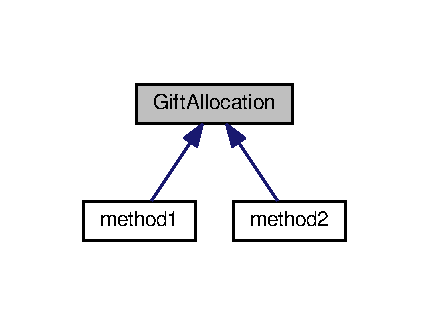
\includegraphics[width=206pt]{classGiftAllocation__inherit__graph}
\end{center}
\end{figure}


Collaboration diagram for Gift\+Allocation\+:
\nopagebreak
\begin{figure}[H]
\begin{center}
\leavevmode
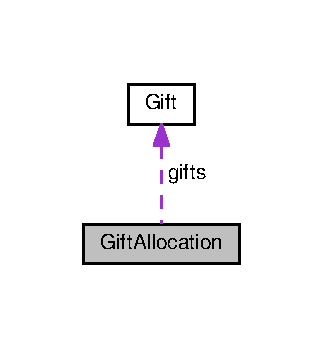
\includegraphics[width=155pt]{classGiftAllocation__coll__graph}
\end{center}
\end{figure}
\subsection*{Public Member Functions}
\begin{DoxyCompactItemize}
\item 
void \hyperlink{classGiftAllocation_a251311eacec6f50e78300c576b3938b9}{take\+Input} ()
\item 
void \hyperlink{classGiftAllocation_a54ab23085223d306af9aa3ded70901be}{sorting\+Gifts} ()
\item 
void \hyperlink{classGiftAllocation_ac75f5851dc71925a5c837c0b35a51d26}{swap} (\hyperlink{classGift}{Gift} \&a, \hyperlink{classGift}{Gift} \&b)
\item 
void \hyperlink{classGiftAllocation_a9ea227b1d051645d9aa54d7c4d4d0ce3}{printing\+Gifts} (\hyperlink{classCouple}{Couple} $\ast$couple)
\end{DoxyCompactItemize}
\subsection*{Public Attributes}
\begin{DoxyCompactItemize}
\item 
\hyperlink{classGift}{Gift} \hyperlink{classGiftAllocation_acb46a98c48d5ba73890195a1bd8b28f5}{gifts} \mbox{[}\hyperlink{Ques9_8cpp_a5e0c07e523d4e77a2cafca06feb836f6}{Gf}\mbox{]}
\end{DoxyCompactItemize}


\subsection{Member Function Documentation}
\index{Gift\+Allocation@{Gift\+Allocation}!printing\+Gifts@{printing\+Gifts}}
\index{printing\+Gifts@{printing\+Gifts}!Gift\+Allocation@{Gift\+Allocation}}
\subsubsection[{\texorpdfstring{printing\+Gifts(\+Couple $\ast$couple)}{printingGifts(Couple *couple)}}]{\setlength{\rightskip}{0pt plus 5cm}void Gift\+Allocation\+::printing\+Gifts (
\begin{DoxyParamCaption}
\item[{{\bf Couple} $\ast$}]{couple}
\end{DoxyParamCaption}
)}\hypertarget{classGiftAllocation_a9ea227b1d051645d9aa54d7c4d4d0ce3}{}\label{classGiftAllocation_a9ea227b1d051645d9aa54d7c4d4d0ce3}

\begin{DoxyCode}
43 \{
44     
45     \textcolor{comment}{//printing assigned gifts}
46     fstream logFile(\textcolor{stringliteral}{"logFile8.dat"}, std::fstream::in | std::fstream::out | std::fstream::app);
47     logFile<<\textcolor{stringliteral}{"\(\backslash\)n\(\backslash\)n-----------------GIFTS ALLOCATION-------------------\(\backslash\)n\(\backslash\)n"};
48 
49     \textcolor{keywordflow}{for}(\textcolor{keywordtype}{int} i = 0 ;i < \hyperlink{dst9_8h_ac4cf4b2ab929bd23951a8676eeac086b}{C}; i++) \{
50         logFile<<\textcolor{stringliteral}{"Boy b"}<<couples[i].getBoy()<<\textcolor{stringliteral}{" gives Girl g"}<<couples[i].getGirl()<<\textcolor{stringliteral}{" the following Gifts
      \(\backslash\)n"};
51         
52         \textcolor{keywordtype}{int} * arr = couples[i].getGifts();
53         \textcolor{keywordflow}{for}(\textcolor{keywordtype}{int} j = 0; j < couples[i].getNum(); j++) \{
54             logFile<<\textcolor{stringliteral}{"G"}<<\hyperlink{classGiftAllocation_acb46a98c48d5ba73890195a1bd8b28f5}{gifts}[arr[j]-1].\hyperlink{classGift_a5b276dda8fab4a4e2618ba82fc8cd787}{getId}()<<\textcolor{stringliteral}{" of worth Rs "}<<
      \hyperlink{classGiftAllocation_acb46a98c48d5ba73890195a1bd8b28f5}{gifts}[arr[j]-1].\hyperlink{classGift_aa36f2b437e93ede1d2569e489b493441}{getprice}()<<\textcolor{stringliteral}{"\(\backslash\)n"};
55         \}
56         logFile<<endl;
57     \}
58 \}
\end{DoxyCode}
\index{Gift\+Allocation@{Gift\+Allocation}!sorting\+Gifts@{sorting\+Gifts}}
\index{sorting\+Gifts@{sorting\+Gifts}!Gift\+Allocation@{Gift\+Allocation}}
\subsubsection[{\texorpdfstring{sorting\+Gifts()}{sortingGifts()}}]{\setlength{\rightskip}{0pt plus 5cm}void Gift\+Allocation\+::sorting\+Gifts (
\begin{DoxyParamCaption}
{}
\end{DoxyParamCaption}
)}\hypertarget{classGiftAllocation_a54ab23085223d306af9aa3ded70901be}{}\label{classGiftAllocation_a54ab23085223d306af9aa3ded70901be}

\begin{DoxyCode}
11 \{
12     \textcolor{comment}{//sorting gifts }
13     \textcolor{keywordflow}{for}(\textcolor{keywordtype}{int} i = 0  ; i< \hyperlink{couple_8h_a5e0c07e523d4e77a2cafca06feb836f6}{Gf}-1; i++) \{
14         \textcolor{keywordflow}{for}(\textcolor{keywordtype}{int} j = i+1; j < \hyperlink{couple_8h_a5e0c07e523d4e77a2cafca06feb836f6}{Gf}; j++) \{
15             \textcolor{keywordflow}{if}(\hyperlink{classGiftAllocation_acb46a98c48d5ba73890195a1bd8b28f5}{gifts}[j].getprice() < \hyperlink{classGiftAllocation_acb46a98c48d5ba73890195a1bd8b28f5}{gifts}[i].getprice()) \{
16                 \hyperlink{classGiftAllocation_ac75f5851dc71925a5c837c0b35a51d26}{swap}(\hyperlink{classGiftAllocation_acb46a98c48d5ba73890195a1bd8b28f5}{gifts}[j],\hyperlink{classGiftAllocation_acb46a98c48d5ba73890195a1bd8b28f5}{gifts}[i]);
17             \}
18         \}
19     \}
20 \}
\end{DoxyCode}
\index{Gift\+Allocation@{Gift\+Allocation}!swap@{swap}}
\index{swap@{swap}!Gift\+Allocation@{Gift\+Allocation}}
\subsubsection[{\texorpdfstring{swap(\+Gift \&a, Gift \&b)}{swap(Gift &a, Gift &b)}}]{\setlength{\rightskip}{0pt plus 5cm}void Gift\+Allocation\+::swap (
\begin{DoxyParamCaption}
\item[{{\bf Gift} \&}]{a, }
\item[{{\bf Gift} \&}]{b}
\end{DoxyParamCaption}
)}\hypertarget{classGiftAllocation_ac75f5851dc71925a5c837c0b35a51d26}{}\label{classGiftAllocation_ac75f5851dc71925a5c837c0b35a51d26}

\begin{DoxyCode}
4 \{
5     \hyperlink{classGift}{Gift} temp = a;
6     a = b;
7     b = temp;
8 \}
\end{DoxyCode}
\index{Gift\+Allocation@{Gift\+Allocation}!take\+Input@{take\+Input}}
\index{take\+Input@{take\+Input}!Gift\+Allocation@{Gift\+Allocation}}
\subsubsection[{\texorpdfstring{take\+Input()}{takeInput()}}]{\setlength{\rightskip}{0pt plus 5cm}void Gift\+Allocation\+::take\+Input (
\begin{DoxyParamCaption}
{}
\end{DoxyParamCaption}
)}\hypertarget{classGiftAllocation_a251311eacec6f50e78300c576b3938b9}{}\label{classGiftAllocation_a251311eacec6f50e78300c576b3938b9}

\begin{DoxyCode}
23 \{
24     \textcolor{keywordtype}{int} c = 0;
25     \textcolor{keywordtype}{int} x = 0;
26     \textcolor{keywordtype}{string} line;
27     ifstream giftInp(\textcolor{stringliteral}{"gift.dat"});
28     \textcolor{keywordflow}{while}(getline(giftInp,line)) \{
29         \textcolor{keywordflow}{if}(c++ == 0) \textcolor{keywordflow}{continue};
30         istringstream iss(line);
31         \textcolor{keywordtype}{int} id,p,v;
32         \textcolor{keywordtype}{char} ty;
33         \textcolor{keywordflow}{if}((iss>>\textcolor{keywordtype}{id}>>p>>ty>>v))\{
34             \hyperlink{classGiftAllocation_acb46a98c48d5ba73890195a1bd8b28f5}{gifts}[x++].\hyperlink{classGift_abc74fbed8b31b5bb7745b3e0c934da9e}{setDetail}(\textcolor{keywordtype}{id},p,ty,0);
35         \} \textcolor{keywordflow}{else} \{
36             \textcolor{keywordflow}{break};
37         \}
38     \}
39     
40 \}
\end{DoxyCode}


\subsection{Member Data Documentation}
\index{Gift\+Allocation@{Gift\+Allocation}!gifts@{gifts}}
\index{gifts@{gifts}!Gift\+Allocation@{Gift\+Allocation}}
\subsubsection[{\texorpdfstring{gifts}{gifts}}]{\setlength{\rightskip}{0pt plus 5cm}{\bf Gift} Gift\+Allocation\+::gifts\mbox{[}{\bf Gf}\mbox{]}}\hypertarget{classGiftAllocation_acb46a98c48d5ba73890195a1bd8b28f5}{}\label{classGiftAllocation_acb46a98c48d5ba73890195a1bd8b28f5}


The documentation for this class was generated from the following files\+:\begin{DoxyCompactItemize}
\item 
\hyperlink{lib8_8h}{lib8.\+h}\item 
\hyperlink{lib8_8cpp}{lib8.\+cpp}\end{DoxyCompactItemize}

\hypertarget{classGirl}{}\section{Girl Class Reference}
\label{classGirl}\index{Girl@{Girl}}


{\ttfamily \#include $<$girl.\+h$>$}

\subsection*{Public Member Functions}
\begin{DoxyCompactItemize}
\item 
string \hyperlink{classGirl_a321ead86446e014c9b513eba8f811feb}{getname} ()
\item 
int \hyperlink{classGirl_afe73c4c4f180aa8f5e0bc4f87455ec0b}{get\+Intelligence} ()
\item 
int \hyperlink{classGirl_a04cfe3e0c21240f92c19152630a40252}{get\+Attractiveness} ()
\item 
int \hyperlink{classGirl_a6192affb0721b385d2c5d83a011a869e}{get\+Maintenance} ()
\item 
int \hyperlink{classGirl_af8412c80e48e58d5e19f85f30300f8cf}{get\+Status} ()
\item 
char \hyperlink{classGirl_af26252dbf5784c2c79744dd4652a3bf2}{get\+Type} ()
\item 
char \hyperlink{classGirl_a9dcd593744beb19f97acc0e3bbff6f76}{get\+Criterion} ()
\item 
void \hyperlink{classGirl_a4bff314dba17278eb1093b15f7be80bd}{set\+Details} (string, int, int, int, char, int, char)
\item 
void \hyperlink{classGirl_a201527323b3fabac4b089f003b8fcc4a}{set\+Status} (int)
\end{DoxyCompactItemize}


\subsection{Member Function Documentation}
\index{Girl@{Girl}!get\+Attractiveness@{get\+Attractiveness}}
\index{get\+Attractiveness@{get\+Attractiveness}!Girl@{Girl}}
\subsubsection[{\texorpdfstring{get\+Attractiveness()}{getAttractiveness()}}]{\setlength{\rightskip}{0pt plus 5cm}int Girl\+::get\+Attractiveness (
\begin{DoxyParamCaption}
{}
\end{DoxyParamCaption}
)}\hypertarget{classGirl_a04cfe3e0c21240f92c19152630a40252}{}\label{classGirl_a04cfe3e0c21240f92c19152630a40252}

\begin{DoxyCode}
13 \{
14         \textcolor{keywordflow}{return} this->attractiveness;
15 \}
\end{DoxyCode}
\index{Girl@{Girl}!get\+Criterion@{get\+Criterion}}
\index{get\+Criterion@{get\+Criterion}!Girl@{Girl}}
\subsubsection[{\texorpdfstring{get\+Criterion()}{getCriterion()}}]{\setlength{\rightskip}{0pt plus 5cm}char Girl\+::get\+Criterion (
\begin{DoxyParamCaption}
{}
\end{DoxyParamCaption}
)}\hypertarget{classGirl_a9dcd593744beb19f97acc0e3bbff6f76}{}\label{classGirl_a9dcd593744beb19f97acc0e3bbff6f76}

\begin{DoxyCode}
33 \{
34     \textcolor{keywordflow}{return} this->criterion;
35 \}
\end{DoxyCode}
\index{Girl@{Girl}!get\+Intelligence@{get\+Intelligence}}
\index{get\+Intelligence@{get\+Intelligence}!Girl@{Girl}}
\subsubsection[{\texorpdfstring{get\+Intelligence()}{getIntelligence()}}]{\setlength{\rightskip}{0pt plus 5cm}int Girl\+::get\+Intelligence (
\begin{DoxyParamCaption}
{}
\end{DoxyParamCaption}
)}\hypertarget{classGirl_afe73c4c4f180aa8f5e0bc4f87455ec0b}{}\label{classGirl_afe73c4c4f180aa8f5e0bc4f87455ec0b}

\begin{DoxyCode}
9 \{
10         \textcolor{keywordflow}{return} this->intelligence;
11 \}
\end{DoxyCode}
\index{Girl@{Girl}!get\+Maintenance@{get\+Maintenance}}
\index{get\+Maintenance@{get\+Maintenance}!Girl@{Girl}}
\subsubsection[{\texorpdfstring{get\+Maintenance()}{getMaintenance()}}]{\setlength{\rightskip}{0pt plus 5cm}int Girl\+::get\+Maintenance (
\begin{DoxyParamCaption}
{}
\end{DoxyParamCaption}
)}\hypertarget{classGirl_a6192affb0721b385d2c5d83a011a869e}{}\label{classGirl_a6192affb0721b385d2c5d83a011a869e}

\begin{DoxyCode}
18 \{
19         \textcolor{keywordflow}{return} this->maintenance;
20 \}
\end{DoxyCode}
\index{Girl@{Girl}!getname@{getname}}
\index{getname@{getname}!Girl@{Girl}}
\subsubsection[{\texorpdfstring{getname()}{getname()}}]{\setlength{\rightskip}{0pt plus 5cm}string Girl\+::getname (
\begin{DoxyParamCaption}
{}
\end{DoxyParamCaption}
)}\hypertarget{classGirl_a321ead86446e014c9b513eba8f811feb}{}\label{classGirl_a321ead86446e014c9b513eba8f811feb}

\begin{DoxyCode}
4 \{
5         \textcolor{keywordflow}{return} this->name;
6 \}
\end{DoxyCode}
\index{Girl@{Girl}!get\+Status@{get\+Status}}
\index{get\+Status@{get\+Status}!Girl@{Girl}}
\subsubsection[{\texorpdfstring{get\+Status()}{getStatus()}}]{\setlength{\rightskip}{0pt plus 5cm}int Girl\+::get\+Status (
\begin{DoxyParamCaption}
{}
\end{DoxyParamCaption}
)}\hypertarget{classGirl_af8412c80e48e58d5e19f85f30300f8cf}{}\label{classGirl_af8412c80e48e58d5e19f85f30300f8cf}

\begin{DoxyCode}
23 \{
24         \textcolor{keywordflow}{return} this->status;
25 \}
\end{DoxyCode}
\index{Girl@{Girl}!get\+Type@{get\+Type}}
\index{get\+Type@{get\+Type}!Girl@{Girl}}
\subsubsection[{\texorpdfstring{get\+Type()}{getType()}}]{\setlength{\rightskip}{0pt plus 5cm}char Girl\+::get\+Type (
\begin{DoxyParamCaption}
{}
\end{DoxyParamCaption}
)}\hypertarget{classGirl_af26252dbf5784c2c79744dd4652a3bf2}{}\label{classGirl_af26252dbf5784c2c79744dd4652a3bf2}

\begin{DoxyCode}
28 \{
29         \textcolor{keywordflow}{return} this->type;
30 \}
\end{DoxyCode}
\index{Girl@{Girl}!set\+Details@{set\+Details}}
\index{set\+Details@{set\+Details}!Girl@{Girl}}
\subsubsection[{\texorpdfstring{set\+Details(string, int, int, int, char, int, char)}{setDetails(string, int, int, int, char, int, char)}}]{\setlength{\rightskip}{0pt plus 5cm}void Girl\+::set\+Details (
\begin{DoxyParamCaption}
\item[{string}]{name, }
\item[{int}]{attractiveness, }
\item[{int}]{intelligence, }
\item[{int}]{maintenance, }
\item[{char}]{type, }
\item[{int}]{status, }
\item[{char}]{criterion}
\end{DoxyParamCaption}
)}\hypertarget{classGirl_a4bff314dba17278eb1093b15f7be80bd}{}\label{classGirl_a4bff314dba17278eb1093b15f7be80bd}

\begin{DoxyCode}
38 \{
39         this->name = name;
40         this->attractiveness = attractiveness;
41         this->intelligence = intelligence;
42         this->maintenance = maintenance;
43         this->type = type;
44         this->status = status;
45     this->criterion = criterion;
46 \}
\end{DoxyCode}
\index{Girl@{Girl}!set\+Status@{set\+Status}}
\index{set\+Status@{set\+Status}!Girl@{Girl}}
\subsubsection[{\texorpdfstring{set\+Status(int)}{setStatus(int)}}]{\setlength{\rightskip}{0pt plus 5cm}void Girl\+::set\+Status (
\begin{DoxyParamCaption}
\item[{int}]{i}
\end{DoxyParamCaption}
)}\hypertarget{classGirl_a201527323b3fabac4b089f003b8fcc4a}{}\label{classGirl_a201527323b3fabac4b089f003b8fcc4a}

\begin{DoxyCode}
47                           \{
48     this->status = i;
49 \}
\end{DoxyCode}


The documentation for this class was generated from the following files\+:\begin{DoxyCompactItemize}
\item 
\hyperlink{girl_8h}{girl.\+h}\item 
\hyperlink{girl_8cpp}{girl.\+cpp}\end{DoxyCompactItemize}

\hypertarget{classLibrary}{}\section{Library Class Reference}
\label{classLibrary}\index{Library@{Library}}


{\ttfamily \#include $<$lib7.\+h$>$}



Collaboration diagram for Library\+:
\nopagebreak
\begin{figure}[H]
\begin{center}
\leavevmode
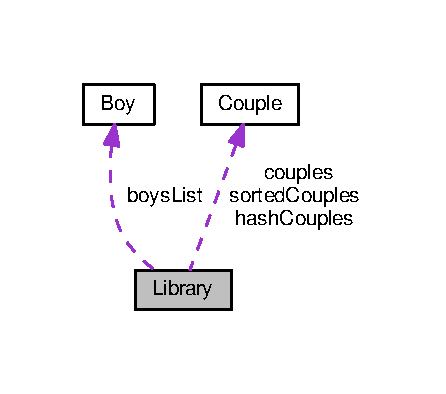
\includegraphics[width=214pt]{classLibrary__coll__graph}
\end{center}
\end{figure}
\subsection*{Public Member Functions}
\begin{DoxyCompactItemize}
\item 
void \hyperlink{classLibrary_af9853cceb7af37b77091c3330b532b2f}{search\+Arr} ()
\item 
void \hyperlink{classLibrary_a835ea2c0b31c569aac4a406843c55254}{search\+Sorted\+Arr} ()
\item 
void \hyperlink{classLibrary_ad14b4301aa6279c13408ff948ca4fd6a}{search\+Hash} ()
\end{DoxyCompactItemize}
\subsection*{Public Attributes}
\begin{DoxyCompactItemize}
\item 
\hyperlink{classCouple}{Couple} $\ast$ \hyperlink{classLibrary_a37cc785266d6a6aeb820499ba875cef1}{couples}
\item 
\hyperlink{classCouple}{Couple} $\ast$ \hyperlink{classLibrary_ac22a9d065ab96fcb3d44e203725e6de6}{sorted\+Couples}
\item 
\hyperlink{classCouple}{Couple} \hyperlink{classLibrary_a81e01bd9f8b2f1fdbc3420b71de2dc49}{hash\+Couples} \mbox{[}\hyperlink{Ques9_8cpp_ac4cf4b2ab929bd23951a8676eeac086b}{C}\mbox{]}
\item 
\hyperlink{classBoy}{Boy} \hyperlink{classLibrary_a28fd1fddb9c961b2cfbb4a054f1ab258}{boys\+List} \mbox{[}\hyperlink{Ques7_8cpp_af933676109efed7ab34cea71d748a517}{S}\mbox{]}
\item 
ofstream \hyperlink{classLibrary_ad8fbb4e17a98e57b3cffe8257710045d}{log\+File}
\end{DoxyCompactItemize}


\subsection{Member Function Documentation}
\index{Library@{Library}!search\+Arr@{search\+Arr}}
\index{search\+Arr@{search\+Arr}!Library@{Library}}
\subsubsection[{\texorpdfstring{search\+Arr()}{searchArr()}}]{\setlength{\rightskip}{0pt plus 5cm}void Library\+::search\+Arr (
\begin{DoxyParamCaption}
{}
\end{DoxyParamCaption}
)}\hypertarget{classLibrary_af9853cceb7af37b77091c3330b532b2f}{}\label{classLibrary_af9853cceb7af37b77091c3330b532b2f}

\begin{DoxyCode}
4 \{   
5 
6     fstream \hyperlink{classLibrary_ad8fbb4e17a98e57b3cffe8257710045d}{logFile}(\textcolor{stringliteral}{"logFile7.dat"}, std::fstream::in | std::fstream::out | std::fstream::app);
7     \hyperlink{classLibrary_ad8fbb4e17a98e57b3cffe8257710045d}{logFile}<<\textcolor{stringliteral}{"\(\backslash\)n----------You selected Linear search------------\(\backslash\)n\(\backslash\)n"};
8     \textcolor{keywordflow}{for}(\textcolor{keywordtype}{int} j = 0; j < \hyperlink{lib7_8h_af933676109efed7ab34cea71d748a517}{S}; j++) \{
9         \textcolor{keywordtype}{int} flag = 0;
10         \textcolor{keywordtype}{int} ind;
11         \textcolor{keywordflow}{for}(\textcolor{keywordtype}{int} i = 0; i < \hyperlink{dst9_8h_ac4cf4b2ab929bd23951a8676eeac086b}{C}; i++) \{
12 
13             \textcolor{keywordflow}{if}(\hyperlink{classLibrary_a37cc785266d6a6aeb820499ba875cef1}{couples}[i].getBoy()[0] == \hyperlink{classLibrary_a28fd1fddb9c961b2cfbb4a054f1ab258}{boysList}[j].getName()[0])\{
14 
15                 flag == 1;
16                 ind = i;        
17                 \hyperlink{classLibrary_ad8fbb4e17a98e57b3cffe8257710045d}{logFile}<<\textcolor{stringliteral}{"Boy b"}<<\hyperlink{classLibrary_a28fd1fddb9c961b2cfbb4a054f1ab258}{boysList}[j].\hyperlink{classBoy_a53e90a641c928c0849e33eca847e902d}{getName}()<<\textcolor{stringliteral}{" is commited with Girl g"}<<
      \hyperlink{classLibrary_a37cc785266d6a6aeb820499ba875cef1}{couples}[ind].\hyperlink{classCouple_a653983df7e331c0534ae2ce42e9856c5}{getGirl}()<<endl; 
18             \} 
19         \}
20     \}
21 
22 \}
\end{DoxyCode}
\index{Library@{Library}!search\+Hash@{search\+Hash}}
\index{search\+Hash@{search\+Hash}!Library@{Library}}
\subsubsection[{\texorpdfstring{search\+Hash()}{searchHash()}}]{\setlength{\rightskip}{0pt plus 5cm}void Library\+::search\+Hash (
\begin{DoxyParamCaption}
{}
\end{DoxyParamCaption}
)}\hypertarget{classLibrary_ad14b4301aa6279c13408ff948ca4fd6a}{}\label{classLibrary_ad14b4301aa6279c13408ff948ca4fd6a}

\begin{DoxyCode}
42 \{
43     fstream \hyperlink{classLibrary_ad8fbb4e17a98e57b3cffe8257710045d}{logFile}(\textcolor{stringliteral}{"logFile7.dat"}, std::fstream::in | std::fstream::out | std::fstream::app);
44     \hyperlink{classLibrary_ad8fbb4e17a98e57b3cffe8257710045d}{logFile}<<\textcolor{stringliteral}{"\(\backslash\)n-----------You selected Hash algorith-----------\(\backslash\)n\(\backslash\)n"};
45     \textcolor{keywordflow}{for}(\textcolor{keywordtype}{int} j = 0; j < \hyperlink{lib7_8h_af933676109efed7ab34cea71d748a517}{S}; j++) \{
46         \textcolor{keywordtype}{int} flag = 0;
47         \textcolor{keywordtype}{int} ind;
48         \textcolor{keywordflow}{for}(\textcolor{keywordtype}{int} i = 0; i < \hyperlink{dst9_8h_ac4cf4b2ab929bd23951a8676eeac086b}{C}; i++) \{
49 
50             \textcolor{keywordflow}{if}(\hyperlink{classLibrary_a81e01bd9f8b2f1fdbc3420b71de2dc49}{hashCouples}[i].getBoy()[0] == \hyperlink{classLibrary_a28fd1fddb9c961b2cfbb4a054f1ab258}{boysList}[j].getName()[0])\{
51 
52                 flag == 1;
53                 ind = i;        
54                 \hyperlink{classLibrary_ad8fbb4e17a98e57b3cffe8257710045d}{logFile}<<\textcolor{stringliteral}{"Boy b"}<<\hyperlink{classLibrary_a28fd1fddb9c961b2cfbb4a054f1ab258}{boysList}[j].\hyperlink{classBoy_a53e90a641c928c0849e33eca847e902d}{getName}()<<\textcolor{stringliteral}{" is commited with Girl g"}<<
      \hyperlink{classLibrary_a81e01bd9f8b2f1fdbc3420b71de2dc49}{hashCouples}[ind].\hyperlink{classCouple_a653983df7e331c0534ae2ce42e9856c5}{getGirl}()<<endl; 
55             \} 
56         \}
57     \}
58 \}
\end{DoxyCode}
\index{Library@{Library}!search\+Sorted\+Arr@{search\+Sorted\+Arr}}
\index{search\+Sorted\+Arr@{search\+Sorted\+Arr}!Library@{Library}}
\subsubsection[{\texorpdfstring{search\+Sorted\+Arr()}{searchSortedArr()}}]{\setlength{\rightskip}{0pt plus 5cm}void Library\+::search\+Sorted\+Arr (
\begin{DoxyParamCaption}
{}
\end{DoxyParamCaption}
)}\hypertarget{classLibrary_a835ea2c0b31c569aac4a406843c55254}{}\label{classLibrary_a835ea2c0b31c569aac4a406843c55254}

\begin{DoxyCode}
24 \{
25     fstream \hyperlink{classLibrary_ad8fbb4e17a98e57b3cffe8257710045d}{logFile}(\textcolor{stringliteral}{"logFile7.dat"}, std::fstream::in | std::fstream::out | std::fstream::app);
26     \hyperlink{classLibrary_ad8fbb4e17a98e57b3cffe8257710045d}{logFile}<<\textcolor{stringliteral}{"\(\backslash\)n--------You selected Binary Search in sorted Array---------\(\backslash\)n\(\backslash\)n"};
27     \textcolor{keywordflow}{for}(\textcolor{keywordtype}{int} j = 0; j < \hyperlink{lib7_8h_af933676109efed7ab34cea71d748a517}{S}; j++) \{
28         \textcolor{keywordtype}{int} flag = 0;
29         \textcolor{keywordtype}{int} ind;
30         \textcolor{keywordflow}{for}(\textcolor{keywordtype}{int} i = 0; i < \hyperlink{dst9_8h_ac4cf4b2ab929bd23951a8676eeac086b}{C}; i++) \{
31 
32             \textcolor{keywordflow}{if}(\hyperlink{classLibrary_ac22a9d065ab96fcb3d44e203725e6de6}{sortedCouples}[i].getBoy()[0] == \hyperlink{classLibrary_a28fd1fddb9c961b2cfbb4a054f1ab258}{boysList}[j].getName()[0])\{
33 
34                 flag == 1;
35                 ind = i;        
36                 \hyperlink{classLibrary_ad8fbb4e17a98e57b3cffe8257710045d}{logFile}<<\textcolor{stringliteral}{"Boy b"}<<\hyperlink{classLibrary_a28fd1fddb9c961b2cfbb4a054f1ab258}{boysList}[j].\hyperlink{classBoy_a53e90a641c928c0849e33eca847e902d}{getName}()<<\textcolor{stringliteral}{" is commited with Girl g"}<<
      \hyperlink{classLibrary_ac22a9d065ab96fcb3d44e203725e6de6}{sortedCouples}[ind].\hyperlink{classCouple_a653983df7e331c0534ae2ce42e9856c5}{getGirl}()<<endl; 
37             \} 
38         \}
39     \}
40 \}
\end{DoxyCode}


\subsection{Member Data Documentation}
\index{Library@{Library}!boys\+List@{boys\+List}}
\index{boys\+List@{boys\+List}!Library@{Library}}
\subsubsection[{\texorpdfstring{boys\+List}{boysList}}]{\setlength{\rightskip}{0pt plus 5cm}{\bf Boy} Library\+::boys\+List\mbox{[}{\bf S}\mbox{]}}\hypertarget{classLibrary_a28fd1fddb9c961b2cfbb4a054f1ab258}{}\label{classLibrary_a28fd1fddb9c961b2cfbb4a054f1ab258}
\index{Library@{Library}!couples@{couples}}
\index{couples@{couples}!Library@{Library}}
\subsubsection[{\texorpdfstring{couples}{couples}}]{\setlength{\rightskip}{0pt plus 5cm}{\bf Couple}$\ast$ Library\+::couples}\hypertarget{classLibrary_a37cc785266d6a6aeb820499ba875cef1}{}\label{classLibrary_a37cc785266d6a6aeb820499ba875cef1}
\index{Library@{Library}!hash\+Couples@{hash\+Couples}}
\index{hash\+Couples@{hash\+Couples}!Library@{Library}}
\subsubsection[{\texorpdfstring{hash\+Couples}{hashCouples}}]{\setlength{\rightskip}{0pt plus 5cm}{\bf Couple} Library\+::hash\+Couples\mbox{[}{\bf C}\mbox{]}}\hypertarget{classLibrary_a81e01bd9f8b2f1fdbc3420b71de2dc49}{}\label{classLibrary_a81e01bd9f8b2f1fdbc3420b71de2dc49}
\index{Library@{Library}!log\+File@{log\+File}}
\index{log\+File@{log\+File}!Library@{Library}}
\subsubsection[{\texorpdfstring{log\+File}{logFile}}]{\setlength{\rightskip}{0pt plus 5cm}ofstream Library\+::log\+File}\hypertarget{classLibrary_ad8fbb4e17a98e57b3cffe8257710045d}{}\label{classLibrary_ad8fbb4e17a98e57b3cffe8257710045d}
\index{Library@{Library}!sorted\+Couples@{sorted\+Couples}}
\index{sorted\+Couples@{sorted\+Couples}!Library@{Library}}
\subsubsection[{\texorpdfstring{sorted\+Couples}{sortedCouples}}]{\setlength{\rightskip}{0pt plus 5cm}{\bf Couple}$\ast$ Library\+::sorted\+Couples}\hypertarget{classLibrary_ac22a9d065ab96fcb3d44e203725e6de6}{}\label{classLibrary_ac22a9d065ab96fcb3d44e203725e6de6}


The documentation for this class was generated from the following files\+:\begin{DoxyCompactItemize}
\item 
\hyperlink{lib7_8h}{lib7.\+h}\item 
\hyperlink{lib7_8cpp}{lib7.\+cpp}\end{DoxyCompactItemize}

\hypertarget{classmethod1}{}\section{method1 Class Reference}
\label{classmethod1}\index{method1@{method1}}


{\ttfamily \#include $<$lib8.\+h$>$}



Inheritance diagram for method1\+:
\nopagebreak
\begin{figure}[H]
\begin{center}
\leavevmode
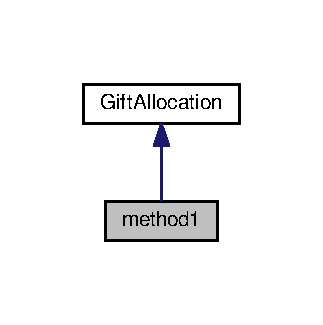
\includegraphics[width=155pt]{classmethod1__inherit__graph}
\end{center}
\end{figure}


Collaboration diagram for method1\+:
\nopagebreak
\begin{figure}[H]
\begin{center}
\leavevmode
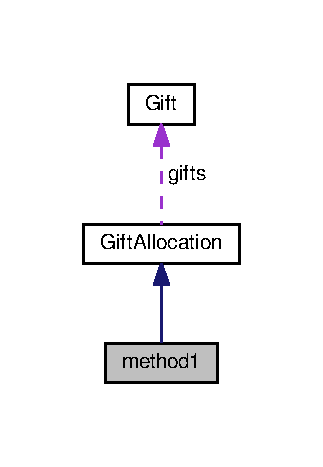
\includegraphics[width=155pt]{classmethod1__coll__graph}
\end{center}
\end{figure}
\subsection*{Public Member Functions}
\begin{DoxyCompactItemize}
\item 
void \hyperlink{classmethod1_a8f2ac4501ad63e68065236359e368864}{allocate} (\hyperlink{classCouple}{Couple} $\ast$couples, \hyperlink{classBoy}{Boy} $\ast$boys, \hyperlink{classGirl}{Girl} $\ast$girls)
\end{DoxyCompactItemize}
\subsection*{Additional Inherited Members}


\subsection{Member Function Documentation}
\index{method1@{method1}!allocate@{allocate}}
\index{allocate@{allocate}!method1@{method1}}
\subsubsection[{\texorpdfstring{allocate(\+Couple $\ast$couples, Boy $\ast$boys, Girl $\ast$girls)}{allocate(Couple *couples, Boy *boys, Girl *girls)}}]{\setlength{\rightskip}{0pt plus 5cm}void method1\+::allocate (
\begin{DoxyParamCaption}
\item[{{\bf Couple} $\ast$}]{couples, }
\item[{{\bf Boy} $\ast$}]{boys, }
\item[{{\bf Girl} $\ast$}]{girls}
\end{DoxyParamCaption}
)}\hypertarget{classmethod1_a8f2ac4501ad63e68065236359e368864}{}\label{classmethod1_a8f2ac4501ad63e68065236359e368864}

\begin{DoxyCode}
62 \{
63     \textcolor{comment}{//Assigning gifts to couples}
64     \textcolor{keywordflow}{for}(\textcolor{keywordtype}{int} i  = 0 ;i < \hyperlink{dst9_8h_ac4cf4b2ab929bd23951a8676eeac086b}{C}; i++) \{
65         \textcolor{keywordtype}{int} boy = couples[i].\hyperlink{classCouple_a092cbc580ea255febc3eb211c5f56512}{getBoy}()[0] - 48;
66         \textcolor{keywordtype}{int} girl = couples[i].\hyperlink{classCouple_a653983df7e331c0534ae2ce42e9856c5}{getGirl}()[0] - 48;
67         \textcolor{keywordtype}{int} mc = girls[girl-1].\hyperlink{classGirl_a6192affb0721b385d2c5d83a011a869e}{getMaintenance}();
68         \textcolor{keywordtype}{int} bud = boys[boy-1].\hyperlink{classBoy_a05c48b12091ebcad44ba86ba88514ac5}{getBudget}();
69         \textcolor{keywordtype}{int} x = bud - mc;
70         \textcolor{keywordtype}{char} bt = boys[boy-1].\hyperlink{classBoy_a01accc077c0824f7e28cfe391f7851c7}{getType}(); 
71     
72         \textcolor{keywordflow}{if}(bt == \textcolor{charliteral}{'M'}) \{
73             \textcolor{keywordflow}{for}(\textcolor{keywordtype}{int} j = 0 ; j < \hyperlink{couple_8h_a5e0c07e523d4e77a2cafca06feb836f6}{Gf}; j++) \{
74                 
75                 \textcolor{keywordflow}{if}(\hyperlink{classGiftAllocation_acb46a98c48d5ba73890195a1bd8b28f5}{gifts}[j].getprice() <= mc && \hyperlink{classGiftAllocation_acb46a98c48d5ba73890195a1bd8b28f5}{gifts}[j].getStatus() == 0) \{
76                     couples[i].\hyperlink{classCouple_a1a621700c479fd808b0caf034f4bd0f5}{setGifts}(j+1);
77                     \hyperlink{classGiftAllocation_acb46a98c48d5ba73890195a1bd8b28f5}{gifts}[j].\hyperlink{classGift_a8c8a8be33c3abe17bbe4b8da9ac084d6}{setStatus}(1);
78                     mc = mc - \hyperlink{classGiftAllocation_acb46a98c48d5ba73890195a1bd8b28f5}{gifts}[j].\hyperlink{classGift_aa36f2b437e93ede1d2569e489b493441}{getprice}();
79                 \} \textcolor{keywordflow}{else} \textcolor{keywordflow}{if}( \hyperlink{classGiftAllocation_acb46a98c48d5ba73890195a1bd8b28f5}{gifts}[j].getprice() <= x +mc ) \{
80                     \textcolor{keywordflow}{if}( \hyperlink{classGiftAllocation_acb46a98c48d5ba73890195a1bd8b28f5}{gifts}[j].getStatus() == 0) \{               
81                         couples[i].\hyperlink{classCouple_a1a621700c479fd808b0caf034f4bd0f5}{setGifts}(j+1);
82                         \hyperlink{classGiftAllocation_acb46a98c48d5ba73890195a1bd8b28f5}{gifts}[j].\hyperlink{classGift_a8c8a8be33c3abe17bbe4b8da9ac084d6}{setStatus}(1);
83                         \textcolor{keywordflow}{break};
84                     \}
85                 \} \textcolor{keywordflow}{else} \{
86                     \textcolor{keywordflow}{break};
87                 \}
88             \} 
89         \} \textcolor{keywordflow}{else}  \textcolor{keywordflow}{if}(bt == \textcolor{charliteral}{'N'}) \{
90             \textcolor{keywordflow}{for}(\textcolor{keywordtype}{int} j = Gf-1 ; j >= 0; j--) \{
91                 \textcolor{keywordflow}{if}(\hyperlink{classGiftAllocation_acb46a98c48d5ba73890195a1bd8b28f5}{gifts}[j].getprice() <= bud && \hyperlink{classGiftAllocation_acb46a98c48d5ba73890195a1bd8b28f5}{gifts}[j].getStatus() == 0) \{
92                     couples[i].\hyperlink{classCouple_a1a621700c479fd808b0caf034f4bd0f5}{setGifts}(j+1);
93                     \hyperlink{classGiftAllocation_acb46a98c48d5ba73890195a1bd8b28f5}{gifts}[j].\hyperlink{classGift_a8c8a8be33c3abe17bbe4b8da9ac084d6}{setStatus}(1);
94                     bud = bud- \hyperlink{classGiftAllocation_acb46a98c48d5ba73890195a1bd8b28f5}{gifts}[j].\hyperlink{classGift_aa36f2b437e93ede1d2569e489b493441}{getprice}();
95                 \}
96             \}
97         \} \textcolor{keywordflow}{else} \{
98             \textcolor{keywordflow}{for}(\textcolor{keywordtype}{int} j = 0 ; j < \hyperlink{couple_8h_a5e0c07e523d4e77a2cafca06feb836f6}{Gf}; j++) \{
99                 \textcolor{keywordflow}{if}(\hyperlink{classGiftAllocation_acb46a98c48d5ba73890195a1bd8b28f5}{gifts}[j].getprice() <= mc && \hyperlink{classGiftAllocation_acb46a98c48d5ba73890195a1bd8b28f5}{gifts}[j].getStatus() == 0) \{
100                     couples[i].\hyperlink{classCouple_a1a621700c479fd808b0caf034f4bd0f5}{setGifts}(j+1);
101                     \hyperlink{classGiftAllocation_acb46a98c48d5ba73890195a1bd8b28f5}{gifts}[j].\hyperlink{classGift_a8c8a8be33c3abe17bbe4b8da9ac084d6}{setStatus}(1);
102                     mc = mc - \hyperlink{classGiftAllocation_acb46a98c48d5ba73890195a1bd8b28f5}{gifts}[j].\hyperlink{classGift_aa36f2b437e93ede1d2569e489b493441}{getprice}();
103                 \}\textcolor{keywordflow}{else} \textcolor{keywordflow}{if}(\hyperlink{classGiftAllocation_acb46a98c48d5ba73890195a1bd8b28f5}{gifts}[j].getprice() <= x +mc) \{
104                     \textcolor{keywordflow}{if}( \hyperlink{classGiftAllocation_acb46a98c48d5ba73890195a1bd8b28f5}{gifts}[j].getStatus() == 0) \{               
105                         couples[i].\hyperlink{classCouple_a1a621700c479fd808b0caf034f4bd0f5}{setGifts}(j+1);
106                         \hyperlink{classGiftAllocation_acb46a98c48d5ba73890195a1bd8b28f5}{gifts}[j].\hyperlink{classGift_a8c8a8be33c3abe17bbe4b8da9ac084d6}{setStatus}(1);
107                         \textcolor{keywordflow}{break};
108                     \}
109                 \} \textcolor{keywordflow}{else} \{
110                     \textcolor{keywordflow}{break};
111                 \}
112             \}
113         \}
114     \}
115 
116     \textcolor{keywordflow}{for}(\textcolor{keywordtype}{int} j = 0 ; j < \hyperlink{couple_8h_a5e0c07e523d4e77a2cafca06feb836f6}{Gf}; j++) \{
117         \hyperlink{classGiftAllocation_acb46a98c48d5ba73890195a1bd8b28f5}{gifts}[j].\hyperlink{classGift_a8c8a8be33c3abe17bbe4b8da9ac084d6}{setStatus}(0);
118     \}
119 
120 \}
\end{DoxyCode}


The documentation for this class was generated from the following files\+:\begin{DoxyCompactItemize}
\item 
\hyperlink{lib8_8h}{lib8.\+h}\item 
\hyperlink{lib8_8cpp}{lib8.\+cpp}\end{DoxyCompactItemize}

\hypertarget{classmethod2}{}\section{method2 Class Reference}
\label{classmethod2}\index{method2@{method2}}


{\ttfamily \#include $<$lib8.\+h$>$}



Inheritance diagram for method2\+:
\nopagebreak
\begin{figure}[H]
\begin{center}
\leavevmode
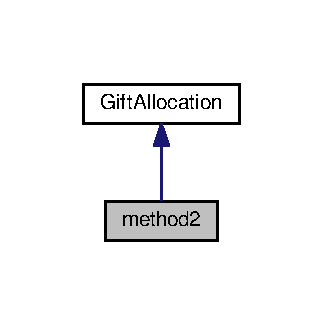
\includegraphics[width=155pt]{classmethod2__inherit__graph}
\end{center}
\end{figure}


Collaboration diagram for method2\+:
\nopagebreak
\begin{figure}[H]
\begin{center}
\leavevmode
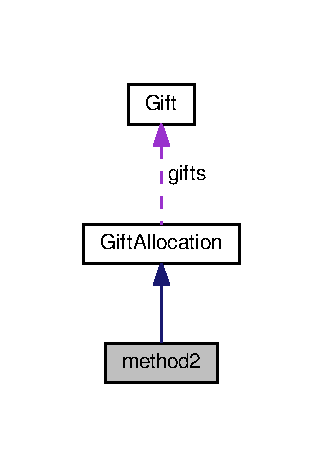
\includegraphics[width=155pt]{classmethod2__coll__graph}
\end{center}
\end{figure}
\subsection*{Public Member Functions}
\begin{DoxyCompactItemize}
\item 
void \hyperlink{classmethod2_af5e7e4483c463a9e13a731d7d56a99f1}{allocate} (\hyperlink{classCouple}{Couple} $\ast$couples, \hyperlink{classBoy}{Boy} $\ast$boys, \hyperlink{classGirl}{Girl} $\ast$girls)
\end{DoxyCompactItemize}
\subsection*{Additional Inherited Members}


\subsection{Member Function Documentation}
\index{method2@{method2}!allocate@{allocate}}
\index{allocate@{allocate}!method2@{method2}}
\subsubsection[{\texorpdfstring{allocate(\+Couple $\ast$couples, Boy $\ast$boys, Girl $\ast$girls)}{allocate(Couple *couples, Boy *boys, Girl *girls)}}]{\setlength{\rightskip}{0pt plus 5cm}void method2\+::allocate (
\begin{DoxyParamCaption}
\item[{{\bf Couple} $\ast$}]{couples, }
\item[{{\bf Boy} $\ast$}]{boys, }
\item[{{\bf Girl} $\ast$}]{girls}
\end{DoxyParamCaption}
)}\hypertarget{classmethod2_af5e7e4483c463a9e13a731d7d56a99f1}{}\label{classmethod2_af5e7e4483c463a9e13a731d7d56a99f1}

\begin{DoxyCode}
123 \{
124     \textcolor{comment}{//Assigning gifts to couples}
125     \textcolor{keywordflow}{for}(\textcolor{keywordtype}{int} i  = 0 ;i < \hyperlink{dst9_8h_ac4cf4b2ab929bd23951a8676eeac086b}{C}; i++) \{
126         \textcolor{keywordtype}{int} boy = couples[i].\hyperlink{classCouple_a092cbc580ea255febc3eb211c5f56512}{getBoy}()[0] - 48;
127         \textcolor{keywordtype}{int} girl = couples[i].\hyperlink{classCouple_a653983df7e331c0534ae2ce42e9856c5}{getGirl}()[0] - 48;
128         \textcolor{keywordtype}{int} mc = girls[girl-1].\hyperlink{classGirl_a6192affb0721b385d2c5d83a011a869e}{getMaintenance}();
129         \textcolor{keywordtype}{int} bud = boys[boy-1].\hyperlink{classBoy_a05c48b12091ebcad44ba86ba88514ac5}{getBudget}();
130         \textcolor{keywordtype}{int} x = bud - mc;
131         \textcolor{keywordtype}{char} bt = boys[boy-1].\hyperlink{classBoy_a01accc077c0824f7e28cfe391f7851c7}{getType}(); 
132     
133         \textcolor{keywordflow}{if}(bt == \textcolor{charliteral}{'N'}) \{
134             \textcolor{keywordflow}{for}(\textcolor{keywordtype}{int} j = 0 ; j < \hyperlink{couple_8h_a5e0c07e523d4e77a2cafca06feb836f6}{Gf}; j++) \{
135                 
136                 \textcolor{keywordflow}{if}(\hyperlink{classGiftAllocation_acb46a98c48d5ba73890195a1bd8b28f5}{gifts}[j].getprice() <= mc && \hyperlink{classGiftAllocation_acb46a98c48d5ba73890195a1bd8b28f5}{gifts}[j].getStatus() == 0) \{
137                     couples[i].\hyperlink{classCouple_a1a621700c479fd808b0caf034f4bd0f5}{setGifts}(j+1);
138                     \hyperlink{classGiftAllocation_acb46a98c48d5ba73890195a1bd8b28f5}{gifts}[j].\hyperlink{classGift_a8c8a8be33c3abe17bbe4b8da9ac084d6}{setStatus}(1);
139                     mc = mc - \hyperlink{classGiftAllocation_acb46a98c48d5ba73890195a1bd8b28f5}{gifts}[j].\hyperlink{classGift_aa36f2b437e93ede1d2569e489b493441}{getprice}();
140                 \} \textcolor{keywordflow}{else} \textcolor{keywordflow}{if}( \hyperlink{classGiftAllocation_acb46a98c48d5ba73890195a1bd8b28f5}{gifts}[j].getprice() <= x +mc ) \{
141                     \textcolor{keywordflow}{if}( \hyperlink{classGiftAllocation_acb46a98c48d5ba73890195a1bd8b28f5}{gifts}[j].getStatus() == 0) \{               
142                         couples[i].\hyperlink{classCouple_a1a621700c479fd808b0caf034f4bd0f5}{setGifts}(j+1);
143                         \hyperlink{classGiftAllocation_acb46a98c48d5ba73890195a1bd8b28f5}{gifts}[j].\hyperlink{classGift_a8c8a8be33c3abe17bbe4b8da9ac084d6}{setStatus}(1);
144                         \textcolor{keywordflow}{break};
145                     \}
146                 \} \textcolor{keywordflow}{else} \{
147                     \textcolor{keywordflow}{break};
148                 \}
149             \} 
150         \} \textcolor{keywordflow}{else}  \textcolor{keywordflow}{if}(bt == \textcolor{charliteral}{'K'}) \{
151             \textcolor{keywordflow}{for}(\textcolor{keywordtype}{int} j = Gf-1 ; j >= 0; j--) \{
152                 \textcolor{keywordflow}{if}(\hyperlink{classGiftAllocation_acb46a98c48d5ba73890195a1bd8b28f5}{gifts}[j].getprice() <= bud && \hyperlink{classGiftAllocation_acb46a98c48d5ba73890195a1bd8b28f5}{gifts}[j].getStatus() == 0) \{
153                     couples[i].\hyperlink{classCouple_a1a621700c479fd808b0caf034f4bd0f5}{setGifts}(j+1);
154                     \hyperlink{classGiftAllocation_acb46a98c48d5ba73890195a1bd8b28f5}{gifts}[j].\hyperlink{classGift_a8c8a8be33c3abe17bbe4b8da9ac084d6}{setStatus}(1);
155                     bud = bud- \hyperlink{classGiftAllocation_acb46a98c48d5ba73890195a1bd8b28f5}{gifts}[j].\hyperlink{classGift_aa36f2b437e93ede1d2569e489b493441}{getprice}();
156                 \}
157             \}
158         \} \textcolor{keywordflow}{else} \{
159             \textcolor{keywordflow}{for}(\textcolor{keywordtype}{int} j = 0 ; j < \hyperlink{couple_8h_a5e0c07e523d4e77a2cafca06feb836f6}{Gf}; j++) \{
160                 \textcolor{keywordflow}{if}(\hyperlink{classGiftAllocation_acb46a98c48d5ba73890195a1bd8b28f5}{gifts}[j].getprice() <= mc && \hyperlink{classGiftAllocation_acb46a98c48d5ba73890195a1bd8b28f5}{gifts}[j].getStatus() == 0) \{
161                     couples[i].\hyperlink{classCouple_a1a621700c479fd808b0caf034f4bd0f5}{setGifts}(j+1);
162                     \hyperlink{classGiftAllocation_acb46a98c48d5ba73890195a1bd8b28f5}{gifts}[j].\hyperlink{classGift_a8c8a8be33c3abe17bbe4b8da9ac084d6}{setStatus}(1);
163                     mc = mc - \hyperlink{classGiftAllocation_acb46a98c48d5ba73890195a1bd8b28f5}{gifts}[j].\hyperlink{classGift_aa36f2b437e93ede1d2569e489b493441}{getprice}();
164                 \}\textcolor{keywordflow}{else} \textcolor{keywordflow}{if}(\hyperlink{classGiftAllocation_acb46a98c48d5ba73890195a1bd8b28f5}{gifts}[j].getprice() <= x +mc) \{
165                     \textcolor{keywordflow}{if}( \hyperlink{classGiftAllocation_acb46a98c48d5ba73890195a1bd8b28f5}{gifts}[j].getStatus() == 0) \{               
166                         couples[i].\hyperlink{classCouple_a1a621700c479fd808b0caf034f4bd0f5}{setGifts}(j+1);
167                         \hyperlink{classGiftAllocation_acb46a98c48d5ba73890195a1bd8b28f5}{gifts}[j].\hyperlink{classGift_a8c8a8be33c3abe17bbe4b8da9ac084d6}{setStatus}(1);
168                         \textcolor{keywordflow}{break};
169                     \}
170                 \} \textcolor{keywordflow}{else} \{
171                     \textcolor{keywordflow}{break};
172                 \}
173             \}
174         \}
175     \}
176 
177     \textcolor{keywordflow}{for}(\textcolor{keywordtype}{int} j = 0 ; j < \hyperlink{couple_8h_a5e0c07e523d4e77a2cafca06feb836f6}{Gf}; j++) \{
178         \hyperlink{classGiftAllocation_acb46a98c48d5ba73890195a1bd8b28f5}{gifts}[j].\hyperlink{classGift_a8c8a8be33c3abe17bbe4b8da9ac084d6}{setStatus}(0);
179     \}
180 
181 \}
\end{DoxyCode}


The documentation for this class was generated from the following files\+:\begin{DoxyCompactItemize}
\item 
\hyperlink{lib8_8h}{lib8.\+h}\item 
\hyperlink{lib8_8cpp}{lib8.\+cpp}\end{DoxyCompactItemize}

\chapter{File Documentation}
\hypertarget{boy_8cpp}{}\section{boy.\+cpp File Reference}
\label{boy_8cpp}\index{boy.\+cpp@{boy.\+cpp}}
{\ttfamily \#include \char`\"{}boy.\+h\char`\"{}}\\*
Include dependency graph for boy.\+cpp\+:
\nopagebreak
\begin{figure}[H]
\begin{center}
\leavevmode
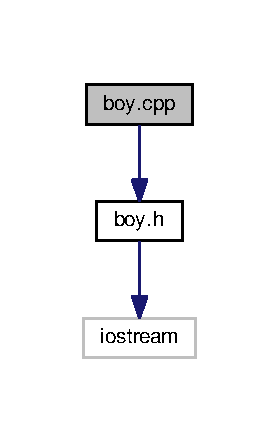
\includegraphics[width=134pt]{boy_8cpp__incl}
\end{center}
\end{figure}

\hypertarget{boy_8h}{}\section{boy.\+h File Reference}
\label{boy_8h}\index{boy.\+h@{boy.\+h}}
{\ttfamily \#include $<$iostream$>$}\\*
Include dependency graph for boy.\+h\+:
\nopagebreak
\begin{figure}[H]
\begin{center}
\leavevmode
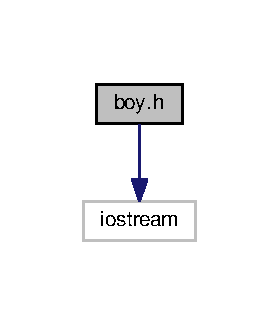
\includegraphics[width=134pt]{boy_8h__incl}
\end{center}
\end{figure}
This graph shows which files directly or indirectly include this file\+:
\nopagebreak
\begin{figure}[H]
\begin{center}
\leavevmode
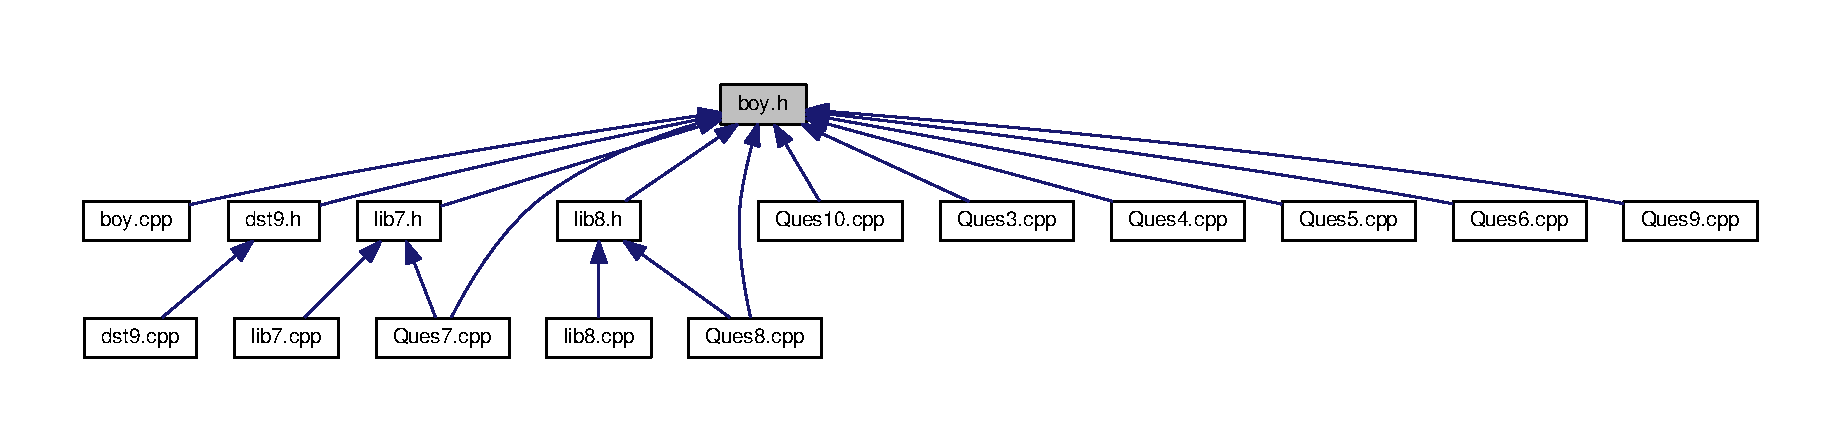
\includegraphics[width=295pt]{boy_8h__dep__incl}
\end{center}
\end{figure}
\subsection*{Classes}
\begin{DoxyCompactItemize}
\item 
class \hyperlink{classBoy}{Boy}
\end{DoxyCompactItemize}

\hypertarget{couple_8cpp}{}\section{couple.\+cpp File Reference}
\label{couple_8cpp}\index{couple.\+cpp@{couple.\+cpp}}
{\ttfamily \#include \char`\"{}couple.\+h\char`\"{}}\\*
Include dependency graph for couple.\+cpp\+:
\nopagebreak
\begin{figure}[H]
\begin{center}
\leavevmode
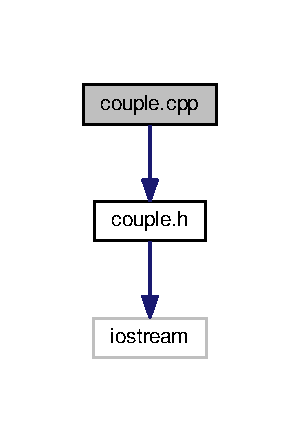
\includegraphics[width=144pt]{couple_8cpp__incl}
\end{center}
\end{figure}

\hypertarget{couple_8h}{}\section{couple.\+h File Reference}
\label{couple_8h}\index{couple.\+h@{couple.\+h}}
{\ttfamily \#include $<$iostream$>$}\\*
Include dependency graph for couple.\+h\+:
\nopagebreak
\begin{figure}[H]
\begin{center}
\leavevmode
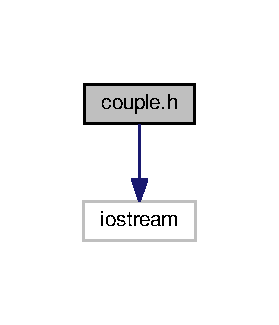
\includegraphics[width=134pt]{couple_8h__incl}
\end{center}
\end{figure}
This graph shows which files directly or indirectly include this file\+:
\nopagebreak
\begin{figure}[H]
\begin{center}
\leavevmode
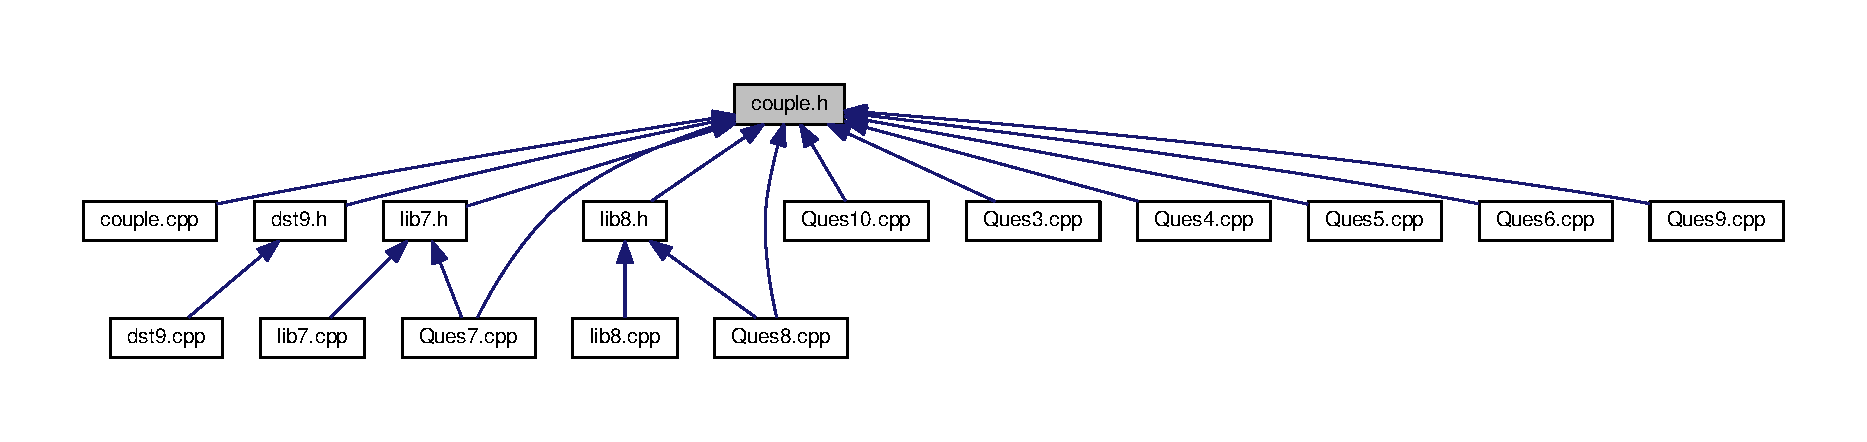
\includegraphics[width=308pt]{couple_8h__dep__incl}
\end{center}
\end{figure}
\subsection*{Classes}
\begin{DoxyCompactItemize}
\item 
class \hyperlink{classCouple}{Couple}
\end{DoxyCompactItemize}
\subsection*{Macros}
\begin{DoxyCompactItemize}
\item 
\#define \hyperlink{couple_8h_a5e0c07e523d4e77a2cafca06feb836f6}{Gf}~15
\end{DoxyCompactItemize}


\subsection{Macro Definition Documentation}
\index{couple.\+h@{couple.\+h}!Gf@{Gf}}
\index{Gf@{Gf}!couple.\+h@{couple.\+h}}
\subsubsection[{\texorpdfstring{Gf}{Gf}}]{\setlength{\rightskip}{0pt plus 5cm}\#define Gf~15}\hypertarget{couple_8h_a5e0c07e523d4e77a2cafca06feb836f6}{}\label{couple_8h_a5e0c07e523d4e77a2cafca06feb836f6}

\hypertarget{dst9_8cpp}{}\section{dst9.\+cpp File Reference}
\label{dst9_8cpp}\index{dst9.\+cpp@{dst9.\+cpp}}
{\ttfamily \#include \char`\"{}dst9.\+h\char`\"{}}\\*
Include dependency graph for dst9.\+cpp\+:
\nopagebreak
\begin{figure}[H]
\begin{center}
\leavevmode
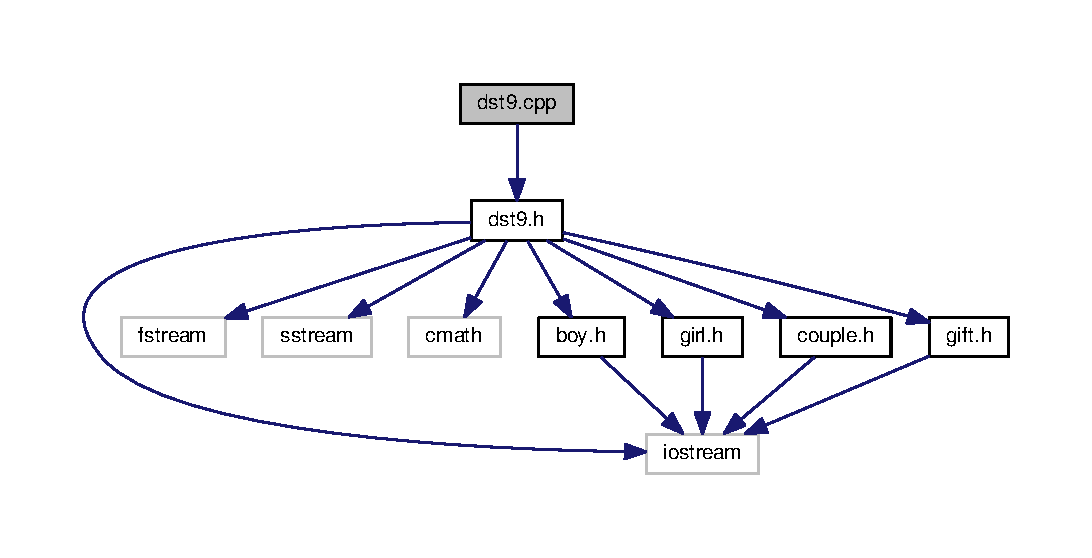
\includegraphics[width=350pt]{dst9_8cpp__incl}
\end{center}
\end{figure}
\subsection*{Functions}
\begin{DoxyCompactItemize}
\item 
{\footnotesize template$<$class T $>$ }\\void \hyperlink{dst9_8cpp_ac2353dbd40ac679cac5ce9213952d284}{swap} (\hyperlink{Ques6_8cpp_a0acb682b8260ab1c60b918599864e2e5}{T} \&a, \hyperlink{Ques6_8cpp_a0acb682b8260ab1c60b918599864e2e5}{T} \&b)
\item 
{\footnotesize template$<$class T $>$ }\\void \hyperlink{dst9_8cpp_afb2bbadfe7cfd2620d67ca6d0ccb2411}{sorting\+Datastructure} (\hyperlink{Ques6_8cpp_a0acb682b8260ab1c60b918599864e2e5}{T} $\ast$arr, int n, int k, string s)
\end{DoxyCompactItemize}


\subsection{Function Documentation}
\index{dst9.\+cpp@{dst9.\+cpp}!sorting\+Datastructure@{sorting\+Datastructure}}
\index{sorting\+Datastructure@{sorting\+Datastructure}!dst9.\+cpp@{dst9.\+cpp}}
\subsubsection[{\texorpdfstring{sorting\+Datastructure(\+T $\ast$arr, int n, int k, string s)}{sortingDatastructure(T *arr, int n, int k, string s)}}]{\setlength{\rightskip}{0pt plus 5cm}template$<$class T $>$ void sorting\+Datastructure (
\begin{DoxyParamCaption}
\item[{{\bf T} $\ast$}]{arr, }
\item[{int}]{n, }
\item[{int}]{k, }
\item[{string}]{s}
\end{DoxyParamCaption}
)}\hypertarget{dst9_8cpp_afb2bbadfe7cfd2620d67ca6d0ccb2411}{}\label{dst9_8cpp_afb2bbadfe7cfd2620d67ca6d0ccb2411}

\begin{DoxyCode}
13 \{
14     \textcolor{keywordflow}{for}(\textcolor{keywordtype}{int} i = 0  ; i< n-1; i++) \{
15         \textcolor{keywordflow}{for}(\textcolor{keywordtype}{int} j = i+1; j < n; j++) \{
16             \textcolor{keywordflow}{if}(s == \textcolor{stringliteral}{"price"}) \{
17                 \textcolor{keywordflow}{if}(arr[j].getprice() < arr[i].getprice()) \{
18                     \hyperlink{dst9_8cpp_ac2353dbd40ac679cac5ce9213952d284}{swap}(arr[j],arr[i]);
19                 \}
20             \} \textcolor{keywordflow}{else} \textcolor{keywordflow}{if}(s == \textcolor{stringliteral}{"attractiveness"}) \{
21                 \textcolor{keywordflow}{if}(arr[j].getAttractiveness() < arr[i].getAttractiveness()) \{
22                     \hyperlink{dst9_8cpp_ac2353dbd40ac679cac5ce9213952d284}{swap}(arr[j],arr[i]);
23                 \}
24             \}
25         \}
26     \}
27 \}
\end{DoxyCode}
\index{dst9.\+cpp@{dst9.\+cpp}!swap@{swap}}
\index{swap@{swap}!dst9.\+cpp@{dst9.\+cpp}}
\subsubsection[{\texorpdfstring{swap(\+T \&a, T \&b)}{swap(T &a, T &b)}}]{\setlength{\rightskip}{0pt plus 5cm}template$<$class T $>$ void swap (
\begin{DoxyParamCaption}
\item[{{\bf T} \&}]{a, }
\item[{{\bf T} \&}]{b}
\end{DoxyParamCaption}
)}\hypertarget{dst9_8cpp_ac2353dbd40ac679cac5ce9213952d284}{}\label{dst9_8cpp_ac2353dbd40ac679cac5ce9213952d284}

\begin{DoxyCode}
5 \{
6     \hyperlink{Ques6_8cpp_a0acb682b8260ab1c60b918599864e2e5}{T} temp = a;
7     a = b;
8     b = temp;
9 \}
\end{DoxyCode}

\hypertarget{dst9_8h}{}\section{dst9.\+h File Reference}
\label{dst9_8h}\index{dst9.\+h@{dst9.\+h}}
{\ttfamily \#include $<$iostream$>$}\\*
{\ttfamily \#include $<$fstream$>$}\\*
{\ttfamily \#include $<$sstream$>$}\\*
{\ttfamily \#include $<$cmath$>$}\\*
{\ttfamily \#include \char`\"{}boy.\+h\char`\"{}}\\*
{\ttfamily \#include \char`\"{}girl.\+h\char`\"{}}\\*
{\ttfamily \#include \char`\"{}couple.\+h\char`\"{}}\\*
{\ttfamily \#include \char`\"{}gift.\+h\char`\"{}}\\*
Include dependency graph for dst9.\+h\+:
\nopagebreak
\begin{figure}[H]
\begin{center}
\leavevmode
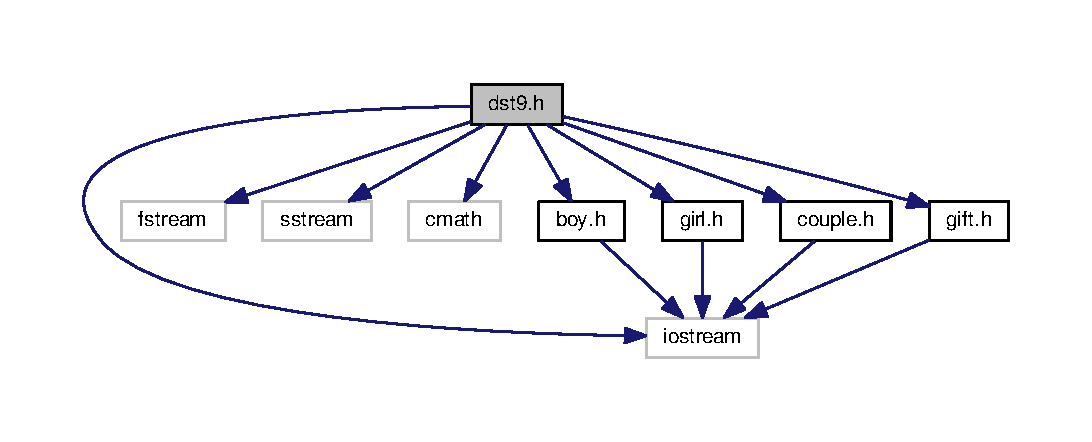
\includegraphics[width=350pt]{dst9_8h__incl}
\end{center}
\end{figure}
This graph shows which files directly or indirectly include this file\+:
\nopagebreak
\begin{figure}[H]
\begin{center}
\leavevmode
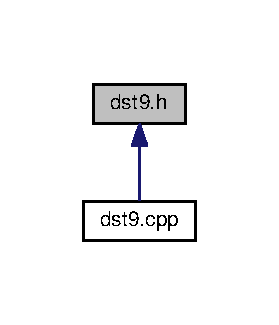
\includegraphics[width=134pt]{dst9_8h__dep__incl}
\end{center}
\end{figure}
\subsection*{Macros}
\begin{DoxyCompactItemize}
\item 
\#define \hyperlink{dst9_8h_a111da81ae5883147168bbb8366377b10}{B}~9
\item 
\#define \hyperlink{dst9_8h_aed9ea78689ecce0b7264c02c7f8a9a54}{G}~5
\item 
\#define \hyperlink{dst9_8h_ac4cf4b2ab929bd23951a8676eeac086b}{C}~5
\item 
\#define \hyperlink{dst9_8h_a5e0c07e523d4e77a2cafca06feb836f6}{Gf}~15
\item 
\#define \hyperlink{dst9_8h_a97d832ae23af4f215e801e37e4f94254}{K}~2
\end{DoxyCompactItemize}
\subsection*{Functions}
\begin{DoxyCompactItemize}
\item 
{\footnotesize template$<$class T $>$ }\\void \hyperlink{dst9_8h_ac2353dbd40ac679cac5ce9213952d284}{swap} (\hyperlink{Ques6_8cpp_a0acb682b8260ab1c60b918599864e2e5}{T} \&a, \hyperlink{Ques6_8cpp_a0acb682b8260ab1c60b918599864e2e5}{T} \&b)
\item 
{\footnotesize template$<$class T $>$ }\\void \hyperlink{dst9_8h_afb2bbadfe7cfd2620d67ca6d0ccb2411}{sorting\+Datastructure} (\hyperlink{Ques6_8cpp_a0acb682b8260ab1c60b918599864e2e5}{T} $\ast$arr, int n, int k, string s)
\end{DoxyCompactItemize}


\subsection{Macro Definition Documentation}
\index{dst9.\+h@{dst9.\+h}!B@{B}}
\index{B@{B}!dst9.\+h@{dst9.\+h}}
\subsubsection[{\texorpdfstring{B}{B}}]{\setlength{\rightskip}{0pt plus 5cm}\#define B~9}\hypertarget{dst9_8h_a111da81ae5883147168bbb8366377b10}{}\label{dst9_8h_a111da81ae5883147168bbb8366377b10}
\index{dst9.\+h@{dst9.\+h}!C@{C}}
\index{C@{C}!dst9.\+h@{dst9.\+h}}
\subsubsection[{\texorpdfstring{C}{C}}]{\setlength{\rightskip}{0pt plus 5cm}\#define C~5}\hypertarget{dst9_8h_ac4cf4b2ab929bd23951a8676eeac086b}{}\label{dst9_8h_ac4cf4b2ab929bd23951a8676eeac086b}
\index{dst9.\+h@{dst9.\+h}!G@{G}}
\index{G@{G}!dst9.\+h@{dst9.\+h}}
\subsubsection[{\texorpdfstring{G}{G}}]{\setlength{\rightskip}{0pt plus 5cm}\#define G~5}\hypertarget{dst9_8h_aed9ea78689ecce0b7264c02c7f8a9a54}{}\label{dst9_8h_aed9ea78689ecce0b7264c02c7f8a9a54}
\index{dst9.\+h@{dst9.\+h}!Gf@{Gf}}
\index{Gf@{Gf}!dst9.\+h@{dst9.\+h}}
\subsubsection[{\texorpdfstring{Gf}{Gf}}]{\setlength{\rightskip}{0pt plus 5cm}\#define Gf~15}\hypertarget{dst9_8h_a5e0c07e523d4e77a2cafca06feb836f6}{}\label{dst9_8h_a5e0c07e523d4e77a2cafca06feb836f6}
\index{dst9.\+h@{dst9.\+h}!K@{K}}
\index{K@{K}!dst9.\+h@{dst9.\+h}}
\subsubsection[{\texorpdfstring{K}{K}}]{\setlength{\rightskip}{0pt plus 5cm}\#define K~2}\hypertarget{dst9_8h_a97d832ae23af4f215e801e37e4f94254}{}\label{dst9_8h_a97d832ae23af4f215e801e37e4f94254}


\subsection{Function Documentation}
\index{dst9.\+h@{dst9.\+h}!sorting\+Datastructure@{sorting\+Datastructure}}
\index{sorting\+Datastructure@{sorting\+Datastructure}!dst9.\+h@{dst9.\+h}}
\subsubsection[{\texorpdfstring{sorting\+Datastructure(\+T $\ast$arr, int n, int k, string s)}{sortingDatastructure(T *arr, int n, int k, string s)}}]{\setlength{\rightskip}{0pt plus 5cm}template$<$class T $>$ void sorting\+Datastructure (
\begin{DoxyParamCaption}
\item[{{\bf T} $\ast$}]{arr, }
\item[{int}]{n, }
\item[{int}]{k, }
\item[{string}]{s}
\end{DoxyParamCaption}
)}\hypertarget{dst9_8h_afb2bbadfe7cfd2620d67ca6d0ccb2411}{}\label{dst9_8h_afb2bbadfe7cfd2620d67ca6d0ccb2411}

\begin{DoxyCode}
13 \{
14     \textcolor{keywordflow}{for}(\textcolor{keywordtype}{int} i = 0  ; i< n-1; i++) \{
15         \textcolor{keywordflow}{for}(\textcolor{keywordtype}{int} j = i+1; j < n; j++) \{
16             \textcolor{keywordflow}{if}(s == \textcolor{stringliteral}{"price"}) \{
17                 \textcolor{keywordflow}{if}(arr[j].getprice() < arr[i].getprice()) \{
18                     \hyperlink{dst9_8cpp_ac2353dbd40ac679cac5ce9213952d284}{swap}(arr[j],arr[i]);
19                 \}
20             \} \textcolor{keywordflow}{else} \textcolor{keywordflow}{if}(s == \textcolor{stringliteral}{"attractiveness"}) \{
21                 \textcolor{keywordflow}{if}(arr[j].getAttractiveness() < arr[i].getAttractiveness()) \{
22                     \hyperlink{dst9_8cpp_ac2353dbd40ac679cac5ce9213952d284}{swap}(arr[j],arr[i]);
23                 \}
24             \}
25         \}
26     \}
27 \}
\end{DoxyCode}
\index{dst9.\+h@{dst9.\+h}!swap@{swap}}
\index{swap@{swap}!dst9.\+h@{dst9.\+h}}
\subsubsection[{\texorpdfstring{swap(\+T \&a, T \&b)}{swap(T &a, T &b)}}]{\setlength{\rightskip}{0pt plus 5cm}template$<$class T $>$ void swap (
\begin{DoxyParamCaption}
\item[{{\bf T} \&}]{a, }
\item[{{\bf T} \&}]{b}
\end{DoxyParamCaption}
)}\hypertarget{dst9_8h_ac2353dbd40ac679cac5ce9213952d284}{}\label{dst9_8h_ac2353dbd40ac679cac5ce9213952d284}

\begin{DoxyCode}
5 \{
6     \hyperlink{Ques6_8cpp_a0acb682b8260ab1c60b918599864e2e5}{T} temp = a;
7     a = b;
8     b = temp;
9 \}
\end{DoxyCode}

\hypertarget{gift_8cpp}{}\section{gift.\+cpp File Reference}
\label{gift_8cpp}\index{gift.\+cpp@{gift.\+cpp}}
{\ttfamily \#include \char`\"{}gift.\+h\char`\"{}}\\*
Include dependency graph for gift.\+cpp\+:
\nopagebreak
\begin{figure}[H]
\begin{center}
\leavevmode
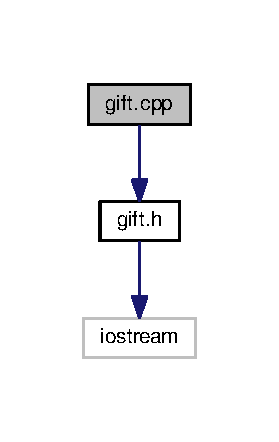
\includegraphics[width=134pt]{gift_8cpp__incl}
\end{center}
\end{figure}

\hypertarget{gift_8h}{}\section{gift.\+h File Reference}
\label{gift_8h}\index{gift.\+h@{gift.\+h}}
{\ttfamily \#include $<$iostream$>$}\\*
Include dependency graph for gift.\+h\+:
\nopagebreak
\begin{figure}[H]
\begin{center}
\leavevmode
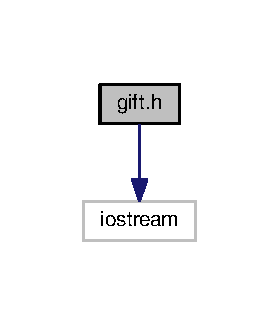
\includegraphics[width=134pt]{gift_8h__incl}
\end{center}
\end{figure}
This graph shows which files directly or indirectly include this file\+:
\nopagebreak
\begin{figure}[H]
\begin{center}
\leavevmode
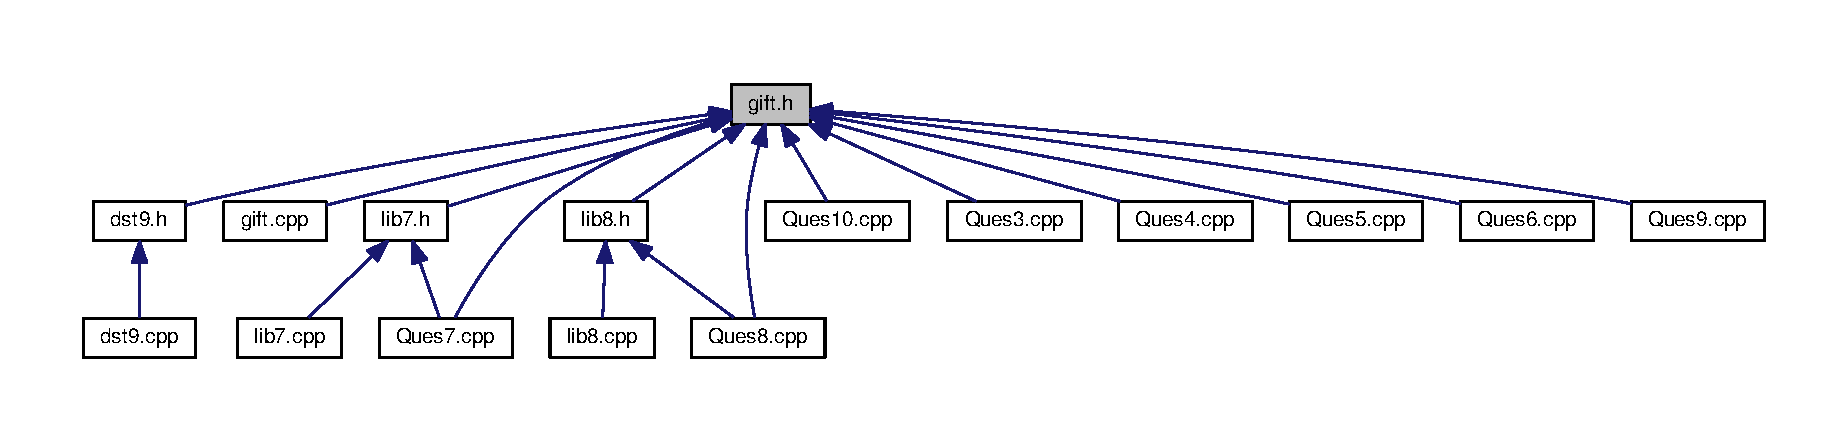
\includegraphics[width=211pt]{gift_8h__dep__incl}
\end{center}
\end{figure}
\subsection*{Classes}
\begin{DoxyCompactItemize}
\item 
class \hyperlink{classGift}{Gift}
\end{DoxyCompactItemize}

\hypertarget{girl_8cpp}{}\section{girl.\+cpp File Reference}
\label{girl_8cpp}\index{girl.\+cpp@{girl.\+cpp}}
{\ttfamily \#include \char`\"{}girl.\+h\char`\"{}}\\*
Include dependency graph for girl.\+cpp\+:
\nopagebreak
\begin{figure}[H]
\begin{center}
\leavevmode
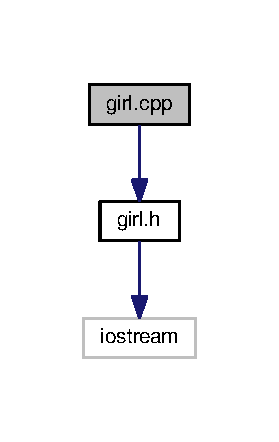
\includegraphics[width=134pt]{girl_8cpp__incl}
\end{center}
\end{figure}

\hypertarget{girl_8h}{}\section{girl.\+h File Reference}
\label{girl_8h}\index{girl.\+h@{girl.\+h}}
{\ttfamily \#include $<$iostream$>$}\\*
Include dependency graph for girl.\+h\+:
\nopagebreak
\begin{figure}[H]
\begin{center}
\leavevmode
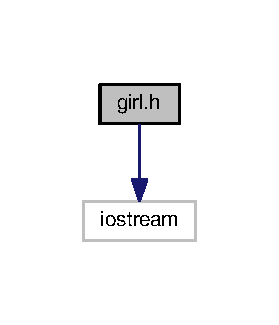
\includegraphics[width=134pt]{girl_8h__incl}
\end{center}
\end{figure}
This graph shows which files directly or indirectly include this file\+:
\nopagebreak
\begin{figure}[H]
\begin{center}
\leavevmode
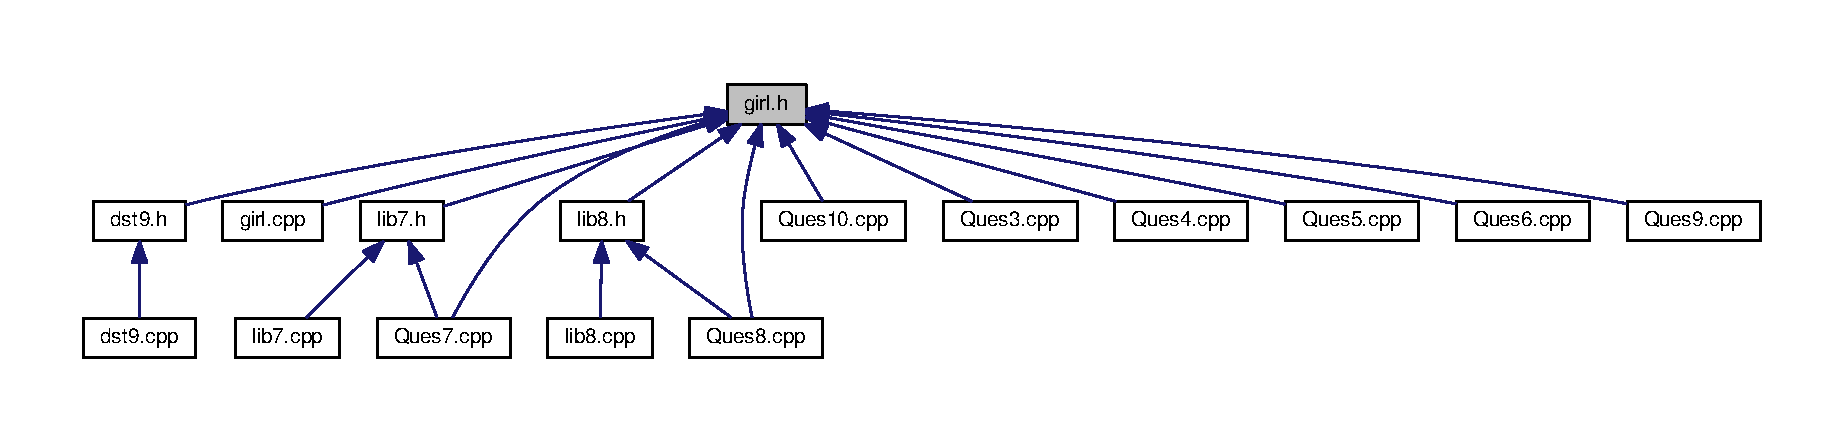
\includegraphics[width=292pt]{girl_8h__dep__incl}
\end{center}
\end{figure}
\subsection*{Classes}
\begin{DoxyCompactItemize}
\item 
class \hyperlink{classGirl}{Girl}
\end{DoxyCompactItemize}

\hypertarget{lib7_8cpp}{}\section{lib7.\+cpp File Reference}
\label{lib7_8cpp}\index{lib7.\+cpp@{lib7.\+cpp}}
{\ttfamily \#include \char`\"{}lib7.\+h\char`\"{}}\\*
Include dependency graph for lib7.\+cpp\+:
\nopagebreak
\begin{figure}[H]
\begin{center}
\leavevmode
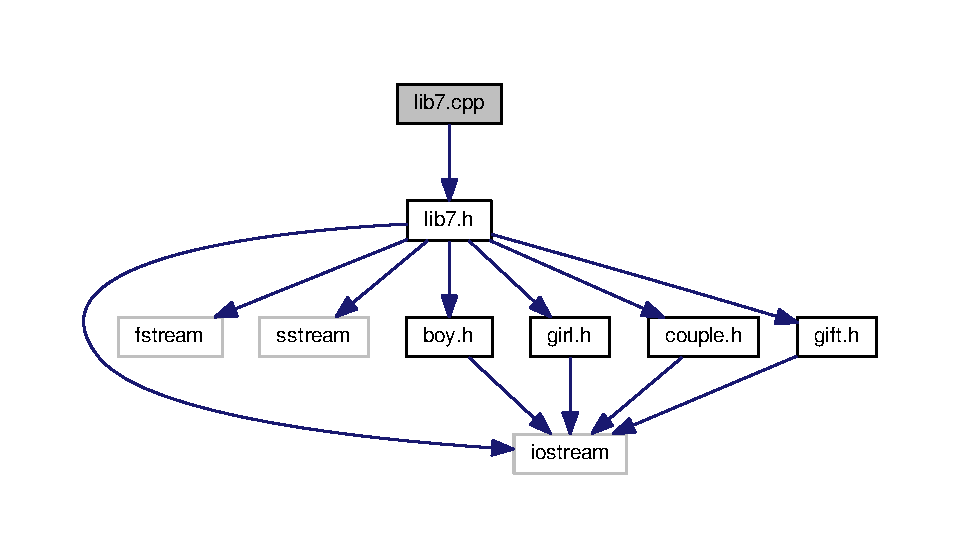
\includegraphics[width=350pt]{lib7_8cpp__incl}
\end{center}
\end{figure}

\hypertarget{lib7_8h}{}\section{lib7.\+h File Reference}
\label{lib7_8h}\index{lib7.\+h@{lib7.\+h}}
{\ttfamily \#include $<$iostream$>$}\\*
{\ttfamily \#include $<$fstream$>$}\\*
{\ttfamily \#include $<$sstream$>$}\\*
{\ttfamily \#include \char`\"{}boy.\+h\char`\"{}}\\*
{\ttfamily \#include \char`\"{}girl.\+h\char`\"{}}\\*
{\ttfamily \#include \char`\"{}couple.\+h\char`\"{}}\\*
{\ttfamily \#include \char`\"{}gift.\+h\char`\"{}}\\*
Include dependency graph for lib7.\+h\+:
\nopagebreak
\begin{figure}[H]
\begin{center}
\leavevmode
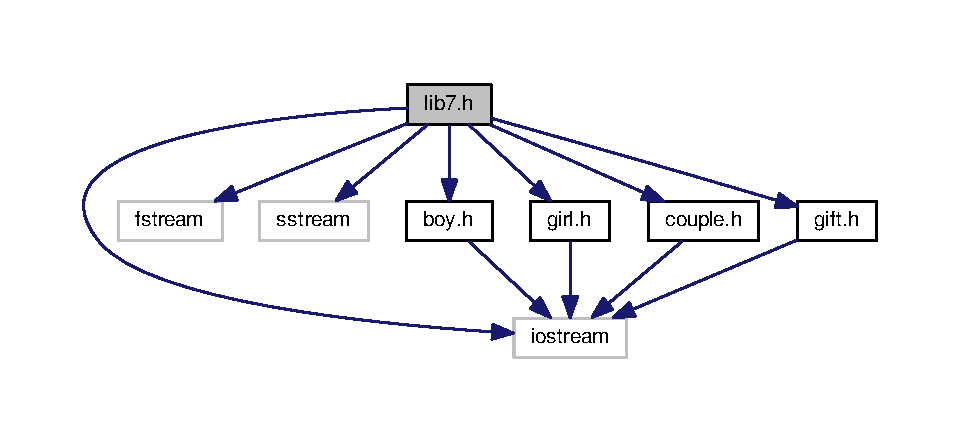
\includegraphics[width=350pt]{lib7_8h__incl}
\end{center}
\end{figure}
This graph shows which files directly or indirectly include this file\+:
\nopagebreak
\begin{figure}[H]
\begin{center}
\leavevmode
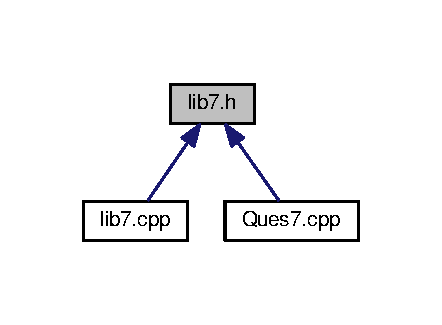
\includegraphics[width=212pt]{lib7_8h__dep__incl}
\end{center}
\end{figure}
\subsection*{Classes}
\begin{DoxyCompactItemize}
\item 
class \hyperlink{classLibrary}{Library}
\end{DoxyCompactItemize}
\subsection*{Macros}
\begin{DoxyCompactItemize}
\item 
\#define \hyperlink{lib7_8h_a111da81ae5883147168bbb8366377b10}{B}~9
\item 
\#define \hyperlink{lib7_8h_aed9ea78689ecce0b7264c02c7f8a9a54}{G}~5
\item 
\#define \hyperlink{lib7_8h_ac4cf4b2ab929bd23951a8676eeac086b}{C}~5
\item 
\#define \hyperlink{lib7_8h_af933676109efed7ab34cea71d748a517}{S}~5
\item 
\#define \hyperlink{lib7_8h_a5e0c07e523d4e77a2cafca06feb836f6}{Gf}~15
\end{DoxyCompactItemize}


\subsection{Macro Definition Documentation}
\index{lib7.\+h@{lib7.\+h}!B@{B}}
\index{B@{B}!lib7.\+h@{lib7.\+h}}
\subsubsection[{\texorpdfstring{B}{B}}]{\setlength{\rightskip}{0pt plus 5cm}\#define B~9}\hypertarget{lib7_8h_a111da81ae5883147168bbb8366377b10}{}\label{lib7_8h_a111da81ae5883147168bbb8366377b10}
\index{lib7.\+h@{lib7.\+h}!C@{C}}
\index{C@{C}!lib7.\+h@{lib7.\+h}}
\subsubsection[{\texorpdfstring{C}{C}}]{\setlength{\rightskip}{0pt plus 5cm}\#define C~5}\hypertarget{lib7_8h_ac4cf4b2ab929bd23951a8676eeac086b}{}\label{lib7_8h_ac4cf4b2ab929bd23951a8676eeac086b}
\index{lib7.\+h@{lib7.\+h}!G@{G}}
\index{G@{G}!lib7.\+h@{lib7.\+h}}
\subsubsection[{\texorpdfstring{G}{G}}]{\setlength{\rightskip}{0pt plus 5cm}\#define G~5}\hypertarget{lib7_8h_aed9ea78689ecce0b7264c02c7f8a9a54}{}\label{lib7_8h_aed9ea78689ecce0b7264c02c7f8a9a54}
\index{lib7.\+h@{lib7.\+h}!Gf@{Gf}}
\index{Gf@{Gf}!lib7.\+h@{lib7.\+h}}
\subsubsection[{\texorpdfstring{Gf}{Gf}}]{\setlength{\rightskip}{0pt plus 5cm}\#define Gf~15}\hypertarget{lib7_8h_a5e0c07e523d4e77a2cafca06feb836f6}{}\label{lib7_8h_a5e0c07e523d4e77a2cafca06feb836f6}
\index{lib7.\+h@{lib7.\+h}!S@{S}}
\index{S@{S}!lib7.\+h@{lib7.\+h}}
\subsubsection[{\texorpdfstring{S}{S}}]{\setlength{\rightskip}{0pt plus 5cm}\#define S~5}\hypertarget{lib7_8h_af933676109efed7ab34cea71d748a517}{}\label{lib7_8h_af933676109efed7ab34cea71d748a517}

\hypertarget{lib8_8cpp}{}\section{lib8.\+cpp File Reference}
\label{lib8_8cpp}\index{lib8.\+cpp@{lib8.\+cpp}}
{\ttfamily \#include \char`\"{}lib8.\+h\char`\"{}}\\*
Include dependency graph for lib8.\+cpp\+:
\nopagebreak
\begin{figure}[H]
\begin{center}
\leavevmode
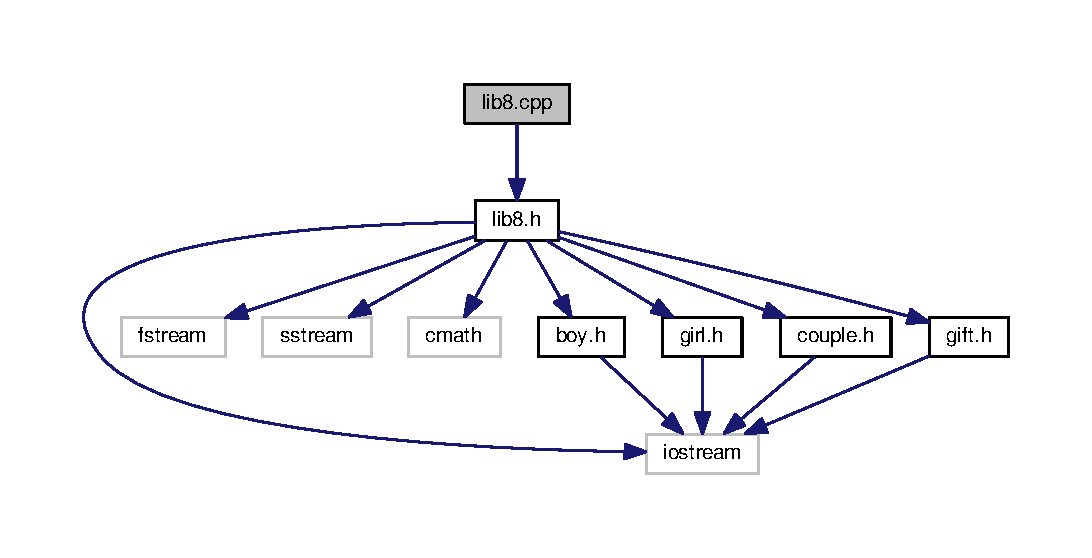
\includegraphics[width=350pt]{lib8_8cpp__incl}
\end{center}
\end{figure}

\hypertarget{lib8_8h}{}\section{lib8.\+h File Reference}
\label{lib8_8h}\index{lib8.\+h@{lib8.\+h}}
{\ttfamily \#include $<$iostream$>$}\\*
{\ttfamily \#include $<$fstream$>$}\\*
{\ttfamily \#include $<$sstream$>$}\\*
{\ttfamily \#include $<$cmath$>$}\\*
{\ttfamily \#include \char`\"{}boy.\+h\char`\"{}}\\*
{\ttfamily \#include \char`\"{}girl.\+h\char`\"{}}\\*
{\ttfamily \#include \char`\"{}couple.\+h\char`\"{}}\\*
{\ttfamily \#include \char`\"{}gift.\+h\char`\"{}}\\*
Include dependency graph for lib8.\+h\+:
\nopagebreak
\begin{figure}[H]
\begin{center}
\leavevmode
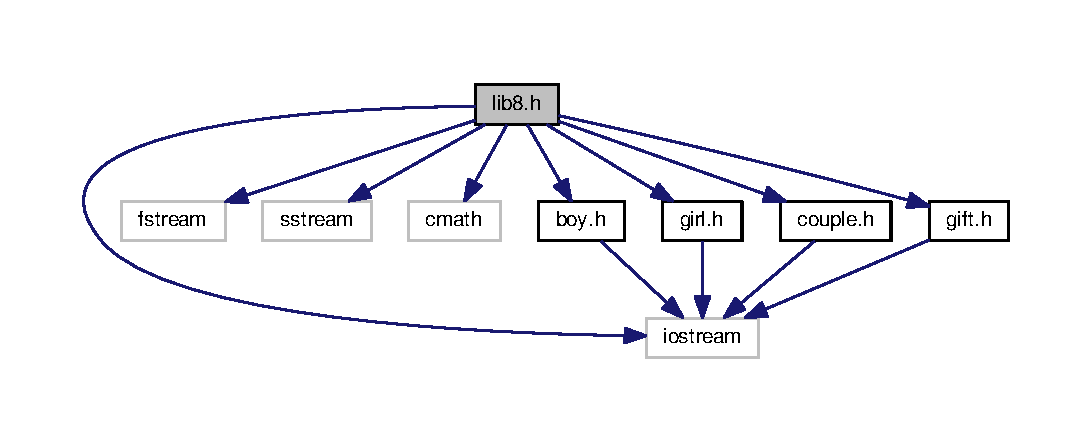
\includegraphics[width=350pt]{lib8_8h__incl}
\end{center}
\end{figure}
This graph shows which files directly or indirectly include this file\+:
\nopagebreak
\begin{figure}[H]
\begin{center}
\leavevmode
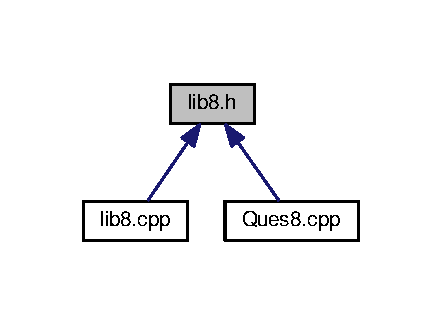
\includegraphics[width=212pt]{lib8_8h__dep__incl}
\end{center}
\end{figure}
\subsection*{Classes}
\begin{DoxyCompactItemize}
\item 
class \hyperlink{classGiftAllocation}{Gift\+Allocation}
\item 
class \hyperlink{classmethod1}{method1}
\item 
class \hyperlink{classmethod2}{method2}
\end{DoxyCompactItemize}
\subsection*{Macros}
\begin{DoxyCompactItemize}
\item 
\#define \hyperlink{lib8_8h_a111da81ae5883147168bbb8366377b10}{B}~9
\item 
\#define \hyperlink{lib8_8h_aed9ea78689ecce0b7264c02c7f8a9a54}{G}~5
\item 
\#define \hyperlink{lib8_8h_ac4cf4b2ab929bd23951a8676eeac086b}{C}~5
\item 
\#define \hyperlink{lib8_8h_a5e0c07e523d4e77a2cafca06feb836f6}{Gf}~15
\item 
\#define \hyperlink{lib8_8h_a97d832ae23af4f215e801e37e4f94254}{K}~2
\end{DoxyCompactItemize}


\subsection{Macro Definition Documentation}
\index{lib8.\+h@{lib8.\+h}!B@{B}}
\index{B@{B}!lib8.\+h@{lib8.\+h}}
\subsubsection[{\texorpdfstring{B}{B}}]{\setlength{\rightskip}{0pt plus 5cm}\#define B~9}\hypertarget{lib8_8h_a111da81ae5883147168bbb8366377b10}{}\label{lib8_8h_a111da81ae5883147168bbb8366377b10}
\index{lib8.\+h@{lib8.\+h}!C@{C}}
\index{C@{C}!lib8.\+h@{lib8.\+h}}
\subsubsection[{\texorpdfstring{C}{C}}]{\setlength{\rightskip}{0pt plus 5cm}\#define C~5}\hypertarget{lib8_8h_ac4cf4b2ab929bd23951a8676eeac086b}{}\label{lib8_8h_ac4cf4b2ab929bd23951a8676eeac086b}
\index{lib8.\+h@{lib8.\+h}!G@{G}}
\index{G@{G}!lib8.\+h@{lib8.\+h}}
\subsubsection[{\texorpdfstring{G}{G}}]{\setlength{\rightskip}{0pt plus 5cm}\#define G~5}\hypertarget{lib8_8h_aed9ea78689ecce0b7264c02c7f8a9a54}{}\label{lib8_8h_aed9ea78689ecce0b7264c02c7f8a9a54}
\index{lib8.\+h@{lib8.\+h}!Gf@{Gf}}
\index{Gf@{Gf}!lib8.\+h@{lib8.\+h}}
\subsubsection[{\texorpdfstring{Gf}{Gf}}]{\setlength{\rightskip}{0pt plus 5cm}\#define Gf~15}\hypertarget{lib8_8h_a5e0c07e523d4e77a2cafca06feb836f6}{}\label{lib8_8h_a5e0c07e523d4e77a2cafca06feb836f6}
\index{lib8.\+h@{lib8.\+h}!K@{K}}
\index{K@{K}!lib8.\+h@{lib8.\+h}}
\subsubsection[{\texorpdfstring{K}{K}}]{\setlength{\rightskip}{0pt plus 5cm}\#define K~2}\hypertarget{lib8_8h_a97d832ae23af4f215e801e37e4f94254}{}\label{lib8_8h_a97d832ae23af4f215e801e37e4f94254}

\hypertarget{Ques10_8cpp}{}\section{Ques10.\+cpp File Reference}
\label{Ques10_8cpp}\index{Ques10.\+cpp@{Ques10.\+cpp}}
{\ttfamily \#include $<$iostream$>$}\\*
{\ttfamily \#include $<$fstream$>$}\\*
{\ttfamily \#include $<$sstream$>$}\\*
{\ttfamily \#include $<$cmath$>$}\\*
{\ttfamily \#include \char`\"{}boy.\+h\char`\"{}}\\*
{\ttfamily \#include \char`\"{}girl.\+h\char`\"{}}\\*
{\ttfamily \#include \char`\"{}couple.\+h\char`\"{}}\\*
{\ttfamily \#include \char`\"{}gift.\+h\char`\"{}}\\*
Include dependency graph for Ques10.\+cpp\+:
\nopagebreak
\begin{figure}[H]
\begin{center}
\leavevmode
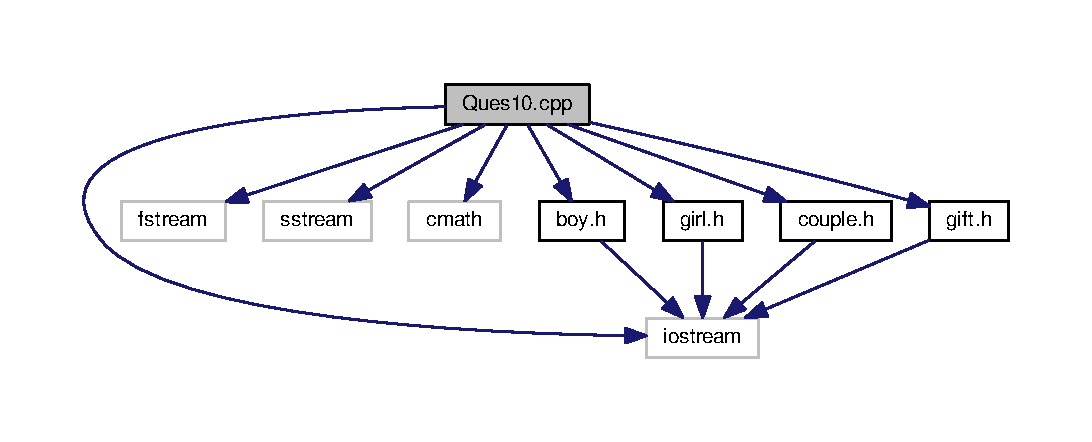
\includegraphics[width=350pt]{Ques10_8cpp__incl}
\end{center}
\end{figure}
\subsection*{Macros}
\begin{DoxyCompactItemize}
\item 
\#define \hyperlink{Ques10_8cpp_a111da81ae5883147168bbb8366377b10}{B}~9
\item 
\#define \hyperlink{Ques10_8cpp_aed9ea78689ecce0b7264c02c7f8a9a54}{G}~5
\item 
\#define \hyperlink{Ques10_8cpp_ac4cf4b2ab929bd23951a8676eeac086b}{C}~5
\item 
\#define \hyperlink{Ques10_8cpp_a5e0c07e523d4e77a2cafca06feb836f6}{Gf}~15
\item 
\#define \hyperlink{Ques10_8cpp_a97d832ae23af4f215e801e37e4f94254}{K}~2
\end{DoxyCompactItemize}
\subsection*{Functions}
\begin{DoxyCompactItemize}
\item 
void \hyperlink{Ques10_8cpp_ac70f752855ee1cf9ceaa2d749bbad17d}{swap} (\hyperlink{classGift}{Gift} \&a, \hyperlink{classGift}{Gift} \&b)
\item 
void \hyperlink{Ques10_8cpp_a9ed5e5ebda90f206f83cd424ebebe79d}{swapC} (\hyperlink{classCouple}{Couple} \&a, \hyperlink{classCouple}{Couple} \&b)
\item 
{\footnotesize template$<$class T $>$ }\\void \hyperlink{Ques10_8cpp_afb2bbadfe7cfd2620d67ca6d0ccb2411}{sorting\+Datastructure} (\hyperlink{Ques6_8cpp_a0acb682b8260ab1c60b918599864e2e5}{T} $\ast$arr, int n, int k, string s)
\item 
int \hyperlink{Ques10_8cpp_ae66f6b31b5ad750f1fe042a706a4e3d4}{main} ()
\end{DoxyCompactItemize}


\subsection{Macro Definition Documentation}
\index{Ques10.\+cpp@{Ques10.\+cpp}!B@{B}}
\index{B@{B}!Ques10.\+cpp@{Ques10.\+cpp}}
\subsubsection[{\texorpdfstring{B}{B}}]{\setlength{\rightskip}{0pt plus 5cm}\#define B~9}\hypertarget{Ques10_8cpp_a111da81ae5883147168bbb8366377b10}{}\label{Ques10_8cpp_a111da81ae5883147168bbb8366377b10}
\index{Ques10.\+cpp@{Ques10.\+cpp}!C@{C}}
\index{C@{C}!Ques10.\+cpp@{Ques10.\+cpp}}
\subsubsection[{\texorpdfstring{C}{C}}]{\setlength{\rightskip}{0pt plus 5cm}\#define C~5}\hypertarget{Ques10_8cpp_ac4cf4b2ab929bd23951a8676eeac086b}{}\label{Ques10_8cpp_ac4cf4b2ab929bd23951a8676eeac086b}
\index{Ques10.\+cpp@{Ques10.\+cpp}!G@{G}}
\index{G@{G}!Ques10.\+cpp@{Ques10.\+cpp}}
\subsubsection[{\texorpdfstring{G}{G}}]{\setlength{\rightskip}{0pt plus 5cm}\#define G~5}\hypertarget{Ques10_8cpp_aed9ea78689ecce0b7264c02c7f8a9a54}{}\label{Ques10_8cpp_aed9ea78689ecce0b7264c02c7f8a9a54}
\index{Ques10.\+cpp@{Ques10.\+cpp}!Gf@{Gf}}
\index{Gf@{Gf}!Ques10.\+cpp@{Ques10.\+cpp}}
\subsubsection[{\texorpdfstring{Gf}{Gf}}]{\setlength{\rightskip}{0pt plus 5cm}\#define Gf~15}\hypertarget{Ques10_8cpp_a5e0c07e523d4e77a2cafca06feb836f6}{}\label{Ques10_8cpp_a5e0c07e523d4e77a2cafca06feb836f6}
\index{Ques10.\+cpp@{Ques10.\+cpp}!K@{K}}
\index{K@{K}!Ques10.\+cpp@{Ques10.\+cpp}}
\subsubsection[{\texorpdfstring{K}{K}}]{\setlength{\rightskip}{0pt plus 5cm}\#define K~2}\hypertarget{Ques10_8cpp_a97d832ae23af4f215e801e37e4f94254}{}\label{Ques10_8cpp_a97d832ae23af4f215e801e37e4f94254}


\subsection{Function Documentation}
\index{Ques10.\+cpp@{Ques10.\+cpp}!main@{main}}
\index{main@{main}!Ques10.\+cpp@{Ques10.\+cpp}}
\subsubsection[{\texorpdfstring{main()}{main()}}]{\setlength{\rightskip}{0pt plus 5cm}int main (
\begin{DoxyParamCaption}
{}
\end{DoxyParamCaption}
)}\hypertarget{Ques10_8cpp_ae66f6b31b5ad750f1fe042a706a4e3d4}{}\label{Ques10_8cpp_ae66f6b31b5ad750f1fe042a706a4e3d4}

\begin{DoxyCode}
51 \{
52     \hyperlink{classBoy}{Boy} boys[\hyperlink{Ques10_8cpp_a111da81ae5883147168bbb8366377b10}{B}];
53     \hyperlink{classGirl}{Girl} girls[\hyperlink{Ques10_8cpp_aed9ea78689ecce0b7264c02c7f8a9a54}{G}];
54     \hyperlink{classCouple}{Couple} couples[\hyperlink{Ques10_8cpp_ac4cf4b2ab929bd23951a8676eeac086b}{C}];
55     \hyperlink{classGift}{Gift} gifts[\hyperlink{Ques10_8cpp_a5e0c07e523d4e77a2cafca06feb836f6}{Gf}];
56     
57     \textcolor{keywordtype}{string} line;
58     \textcolor{keywordtype}{int} c = 0, x = 0;
59 
60     ofstream logFile;
61     logFile.open(\textcolor{stringliteral}{"logFile10.dat"});
62 
63 
64     \textcolor{comment}{//taking input from boy.dat}
65     ifstream boyInp(\textcolor{stringliteral}{"boy.dat"});
66     \textcolor{keywordflow}{while}(getline(boyInp,line)) \{
67         \textcolor{keywordflow}{if}(c++ == 0) \textcolor{keywordflow}{continue};
68         istringstream iss(line);
69         \textcolor{keywordtype}{string} name;
70         \textcolor{keywordtype}{int} a,i,b,t,s;
71         \textcolor{keywordtype}{char} ty;
72         \textcolor{keywordflow}{if}((iss>>name>>a>>i>>b>>t>>s>>ty))\{
73             boys[x++].\hyperlink{classBoy_a6ac70867d517f6b429ce67c8eb2915ed}{setDetails}(name,a,i,b,t,s,ty);
74         \} \textcolor{keywordflow}{else} \{
75             \textcolor{keywordflow}{break};
76         \}
77     \}
78 
79     c = 0;
80     x = 0;
81     \textcolor{comment}{//taking input from girl.dat}
82     ifstream girlInp(\textcolor{stringliteral}{"girl.dat"});
83     \textcolor{keywordflow}{while}(getline(girlInp,line)) \{
84         \textcolor{keywordflow}{if}(c++ == 0) \textcolor{keywordflow}{continue};
85         istringstream iss(line);
86         \textcolor{keywordtype}{string} name;
87         \textcolor{keywordtype}{int} a,i,m,s;
88         \textcolor{keywordtype}{char} ty,cr;
89         \textcolor{keywordflow}{if}((iss>>name>>a>>i>>m>>cr>>s>>ty))\{
90             girls[x++].\hyperlink{classGirl_a4bff314dba17278eb1093b15f7be80bd}{setDetails}(name,a,i,m,ty,s,cr);
91         \} \textcolor{keywordflow}{else} \{
92             \textcolor{keywordflow}{break};
93         \}
94     \}
95 
96     c = 0;
97     x = 0;
98     \textcolor{comment}{//taking input gift.dat}
99     ifstream giftInp(\textcolor{stringliteral}{"gift.dat"});
100     \textcolor{keywordflow}{while}(getline(giftInp,line)) \{
101         \textcolor{keywordflow}{if}(c++ == 0) \textcolor{keywordflow}{continue};
102         istringstream iss(line);
103         \textcolor{keywordtype}{int} id,p,v;
104         \textcolor{keywordtype}{char} ty;
105         \textcolor{keywordflow}{if}((iss>>\textcolor{keywordtype}{id}>>p>>ty>>v))\{
106             gifts[x++].\hyperlink{classGift_abc74fbed8b31b5bb7745b3e0c934da9e}{setDetail}(\textcolor{keywordtype}{id},p,ty,0);
107         \} \textcolor{keywordflow}{else} \{
108             \textcolor{keywordflow}{break};
109         \}
110     \}
111     
112     c = 0;
113     \textcolor{comment}{//forming couples}
114     \textcolor{keywordflow}{for}(\textcolor{keywordtype}{int} i = 0 ; i < \hyperlink{Ques10_8cpp_aed9ea78689ecce0b7264c02c7f8a9a54}{G}; i++) \{
115         \textcolor{keywordtype}{int} k = \hyperlink{Ques10_8cpp_aed9ea78689ecce0b7264c02c7f8a9a54}{G};
116         \hyperlink{Ques10_8cpp_afb2bbadfe7cfd2620d67ca6d0ccb2411}{sortingDatastructure}(girls,G,k,\textcolor{stringliteral}{"attractiveness"});
117         \textcolor{keywordtype}{int} ind = 0; 
118         \textcolor{keywordtype}{int} min = 999999;   
119         \textcolor{keywordflow}{for}(\textcolor{keywordtype}{int} j = 0; j< k ; j++) \{
120             \textcolor{keywordflow}{if}(girls[j].getMaintenance() < min && girls[j].getStatus() == 0)
121             \{
122                 ind = j;
123             \} 
124         \}
125         boys[i].\hyperlink{classBoy_a3d29dcc4137fbfc0306cbd7df82781c3}{setStatus}(1);
126                 girls[ind].\hyperlink{classGirl_a201527323b3fabac4b089f003b8fcc4a}{setStatus}(1);
127                 couples[c++].\hyperlink{classCouple_a0057d3dfd3939a156cd99f6c5cf32279}{setDetails}(boys[i].getName(),girls[ind].getname()) ;
128     \}
129 
130     \textcolor{comment}{//printing couples}
131     logFile<<\textcolor{stringliteral}{"-----------------COUPLES-------------------\(\backslash\)n\(\backslash\)n"};
132 
133     \textcolor{keywordflow}{for}(\textcolor{keywordtype}{int} i = 0 ;i < \hyperlink{Ques10_8cpp_ac4cf4b2ab929bd23951a8676eeac086b}{C}; i++) \{
134         logFile<<\textcolor{stringliteral}{"Boy b"}<<couples[i].\hyperlink{classCouple_a092cbc580ea255febc3eb211c5f56512}{getBoy}()<<\textcolor{stringliteral}{" and Girl g"}<<couples[i].
      \hyperlink{classCouple_a653983df7e331c0534ae2ce42e9856c5}{getGirl}()<<\textcolor{stringliteral}{"\(\backslash\)n"};
135         
136     \}
137 
138     \textcolor{comment}{//sorting gifts }
139     \textcolor{keywordflow}{for}(\textcolor{keywordtype}{int} i = 0  ; i< \hyperlink{Ques10_8cpp_a5e0c07e523d4e77a2cafca06feb836f6}{Gf}-1; i++) \{
140         \textcolor{keywordflow}{for}(\textcolor{keywordtype}{int} j = i+1; j < \hyperlink{Ques10_8cpp_a5e0c07e523d4e77a2cafca06feb836f6}{Gf}; j++) \{
141             \textcolor{keywordflow}{if}(gifts[j].getprice() < gifts[i].getprice()) \{
142                 \hyperlink{Ques10_8cpp_ac70f752855ee1cf9ceaa2d749bbad17d}{swap}(gifts[j],gifts[i]);
143             \}
144         \}
145     \}
146 
147     \textcolor{comment}{//Assigning gifts to couples}
148     \textcolor{keywordflow}{for}(\textcolor{keywordtype}{int} i  = 0 ;i < \hyperlink{Ques10_8cpp_ac4cf4b2ab929bd23951a8676eeac086b}{C}; i++) \{
149         \textcolor{keywordtype}{int} boy = couples[i].\hyperlink{classCouple_a092cbc580ea255febc3eb211c5f56512}{getBoy}()[0] - 48;
150         \textcolor{keywordtype}{int} girl = couples[i].\hyperlink{classCouple_a653983df7e331c0534ae2ce42e9856c5}{getGirl}()[0] - 48;
151         \textcolor{keywordtype}{int} mc = girls[girl-1].\hyperlink{classGirl_a6192affb0721b385d2c5d83a011a869e}{getMaintenance}();
152         \textcolor{keywordtype}{int} bud = boys[boy-1].\hyperlink{classBoy_a05c48b12091ebcad44ba86ba88514ac5}{getBudget}();
153         \textcolor{keywordtype}{int} x = bud - mc;
154         \textcolor{keywordtype}{char} bt = boys[boy-1].\hyperlink{classBoy_a01accc077c0824f7e28cfe391f7851c7}{getType}(); 
155     
156         \textcolor{keywordflow}{if}(bt == \textcolor{charliteral}{'M'}) \{
157             \textcolor{keywordflow}{for}(\textcolor{keywordtype}{int} j = 0 ; j < \hyperlink{Ques10_8cpp_a5e0c07e523d4e77a2cafca06feb836f6}{Gf}; j++) \{
158                 
159                 \textcolor{keywordflow}{if}(gifts[j].getprice() <= mc && gifts[j].getStatus() == 0) \{
160                     couples[i].\hyperlink{classCouple_a1a621700c479fd808b0caf034f4bd0f5}{setGifts}(j+1);
161                     gifts[j].\hyperlink{classGift_a8c8a8be33c3abe17bbe4b8da9ac084d6}{setStatus}(1);
162                     mc = mc - gifts[j].\hyperlink{classGift_aa36f2b437e93ede1d2569e489b493441}{getprice}();
163                 \} \textcolor{keywordflow}{else} \textcolor{keywordflow}{if}( gifts[j].getprice() <= x +mc ) \{
164                     \textcolor{keywordflow}{if}( gifts[j].getStatus() == 0)  \{               
165                         couples[i].\hyperlink{classCouple_a1a621700c479fd808b0caf034f4bd0f5}{setGifts}(j+1);
166                         gifts[j].\hyperlink{classGift_a8c8a8be33c3abe17bbe4b8da9ac084d6}{setStatus}(1);
167                         \textcolor{keywordflow}{break};
168                     \}
169                 \} \textcolor{keywordflow}{else} \{
170                     \textcolor{keywordflow}{break};
171                 \}
172             \} 
173         \} \textcolor{keywordflow}{else}  \textcolor{keywordflow}{if}(bt == \textcolor{charliteral}{'N'}) \{
174             \textcolor{keywordflow}{for}(\textcolor{keywordtype}{int} j = Gf-1 ; j >= 0; j--) \{
175                 \textcolor{keywordflow}{if}(gifts[j].getprice() <= bud && gifts[j].getStatus() == 0) \{
176                     couples[i].\hyperlink{classCouple_a1a621700c479fd808b0caf034f4bd0f5}{setGifts}(j+1);
177                     gifts[j].\hyperlink{classGift_a8c8a8be33c3abe17bbe4b8da9ac084d6}{setStatus}(1);
178                     bud = bud- gifts[j].\hyperlink{classGift_aa36f2b437e93ede1d2569e489b493441}{getprice}();
179                 \}
180             \}
181         \} \textcolor{keywordflow}{else} \{
182             \textcolor{keywordflow}{for}(\textcolor{keywordtype}{int} j = 0 ; j < \hyperlink{Ques10_8cpp_a5e0c07e523d4e77a2cafca06feb836f6}{Gf}; j++) \{
183                 \textcolor{keywordflow}{if}(gifts[j].getprice() <= mc && gifts[j].getStatus() == 0) \{
184                     couples[i].\hyperlink{classCouple_a1a621700c479fd808b0caf034f4bd0f5}{setGifts}(j+1);
185                     gifts[j].\hyperlink{classGift_a8c8a8be33c3abe17bbe4b8da9ac084d6}{setStatus}(1);
186                     mc = mc - gifts[j].\hyperlink{classGift_aa36f2b437e93ede1d2569e489b493441}{getprice}();
187                 \}\textcolor{keywordflow}{else} \textcolor{keywordflow}{if}(gifts[j].getprice() <= x +mc) \{
188                     \textcolor{keywordflow}{if}( gifts[j].getStatus() == 0)  \{               
189                         couples[i].\hyperlink{classCouple_a1a621700c479fd808b0caf034f4bd0f5}{setGifts}(j+1);
190                         gifts[j].\hyperlink{classGift_a8c8a8be33c3abe17bbe4b8da9ac084d6}{setStatus}(1);
191                         \textcolor{keywordflow}{break};
192                     \}
193                 \} \textcolor{keywordflow}{else} \{
194                     \textcolor{keywordflow}{break};
195                 \}
196             \}
197         \}
198     \}
199     
200     \textcolor{comment}{//printing assigned gifts}
201     logFile<<\textcolor{stringliteral}{"\(\backslash\)n\(\backslash\)n-----------------GIFTS ALLOCATION-------------------\(\backslash\)n\(\backslash\)n"};
202 
203     \textcolor{keywordflow}{for}(\textcolor{keywordtype}{int} i = 0 ;i < \hyperlink{Ques10_8cpp_ac4cf4b2ab929bd23951a8676eeac086b}{C}; i++) \{
204         logFile<<\textcolor{stringliteral}{"Boy b"}<<couples[i].\hyperlink{classCouple_a092cbc580ea255febc3eb211c5f56512}{getBoy}()<<\textcolor{stringliteral}{" gives Girl g"}<<couples[i].
      \hyperlink{classCouple_a653983df7e331c0534ae2ce42e9856c5}{getGirl}()<<\textcolor{stringliteral}{" the following Gifts\(\backslash\)n"};
205         
206         \textcolor{keywordtype}{int} * arr = couples[i].\hyperlink{classCouple_a80cef2647acb3903936372a0d70cf9cc}{getGifts}();
207         \textcolor{keywordflow}{for}(\textcolor{keywordtype}{int} j = 0; j < couples[i].\hyperlink{classCouple_a05a3bbd0d8d6b149ae04f5306acd4439}{getNum}(); j++) \{
208             logFile<<\textcolor{stringliteral}{"G"}<<gifts[arr[j]-1].\hyperlink{classGift_a5b276dda8fab4a4e2618ba82fc8cd787}{getId}()<<\textcolor{stringliteral}{" of worth Rs "}<<gifts[arr[j]-1].
      \hyperlink{classGift_aa36f2b437e93ede1d2569e489b493441}{getprice}()<<\textcolor{stringliteral}{"\(\backslash\)n"};
209         \}
210         logFile<<endl;
211     \}
212 
213     logFile.close();
214 \}
\end{DoxyCode}
\index{Ques10.\+cpp@{Ques10.\+cpp}!sorting\+Datastructure@{sorting\+Datastructure}}
\index{sorting\+Datastructure@{sorting\+Datastructure}!Ques10.\+cpp@{Ques10.\+cpp}}
\subsubsection[{\texorpdfstring{sorting\+Datastructure(\+T $\ast$arr, int n, int k, string s)}{sortingDatastructure(T *arr, int n, int k, string s)}}]{\setlength{\rightskip}{0pt plus 5cm}template$<$class T $>$ void sorting\+Datastructure (
\begin{DoxyParamCaption}
\item[{{\bf T} $\ast$}]{arr, }
\item[{int}]{n, }
\item[{int}]{k, }
\item[{string}]{s}
\end{DoxyParamCaption}
)}\hypertarget{Ques10_8cpp_afb2bbadfe7cfd2620d67ca6d0ccb2411}{}\label{Ques10_8cpp_afb2bbadfe7cfd2620d67ca6d0ccb2411}

\begin{DoxyCode}
37 \{
38     \textcolor{keywordflow}{for}(\textcolor{keywordtype}{int} i = 0  ; i< n-1; i++) \{
39         \textcolor{keywordflow}{for}(\textcolor{keywordtype}{int} j = i+1; j < n; j++) \{
40              \textcolor{keywordflow}{if}(s == \textcolor{stringliteral}{"attractiveness"}) \{
41                 \textcolor{keywordflow}{if}(arr[j].getAttractiveness() < arr[i].getAttractiveness()) \{
42                     \hyperlink{Ques10_8cpp_ac70f752855ee1cf9ceaa2d749bbad17d}{swap}(arr[j],arr[i]);
43                 \}
44             \}
45         \}
46     \}
47 \}
\end{DoxyCode}
\index{Ques10.\+cpp@{Ques10.\+cpp}!swap@{swap}}
\index{swap@{swap}!Ques10.\+cpp@{Ques10.\+cpp}}
\subsubsection[{\texorpdfstring{swap(\+Gift \&a, Gift \&b)}{swap(Gift &a, Gift &b)}}]{\setlength{\rightskip}{0pt plus 5cm}void swap (
\begin{DoxyParamCaption}
\item[{{\bf Gift} \&}]{a, }
\item[{{\bf Gift} \&}]{b}
\end{DoxyParamCaption}
)}\hypertarget{Ques10_8cpp_ac70f752855ee1cf9ceaa2d749bbad17d}{}\label{Ques10_8cpp_ac70f752855ee1cf9ceaa2d749bbad17d}

\begin{DoxyCode}
21 \{
22     \hyperlink{classGift}{Gift} temp = a;
23     a = b;
24     b = temp;
25 \}
\end{DoxyCode}
\index{Ques10.\+cpp@{Ques10.\+cpp}!swapC@{swapC}}
\index{swapC@{swapC}!Ques10.\+cpp@{Ques10.\+cpp}}
\subsubsection[{\texorpdfstring{swap\+C(\+Couple \&a, Couple \&b)}{swapC(Couple &a, Couple &b)}}]{\setlength{\rightskip}{0pt plus 5cm}void swapC (
\begin{DoxyParamCaption}
\item[{{\bf Couple} \&}]{a, }
\item[{{\bf Couple} \&}]{b}
\end{DoxyParamCaption}
)}\hypertarget{Ques10_8cpp_a9ed5e5ebda90f206f83cd424ebebe79d}{}\label{Ques10_8cpp_a9ed5e5ebda90f206f83cd424ebebe79d}

\begin{DoxyCode}
28 \{
29     \hyperlink{classCouple}{Couple} temp = a;
30     a = b;
31     b = temp;
32 \}
\end{DoxyCode}

\hypertarget{Ques3_8cpp}{}\section{Ques3.\+cpp File Reference}
\label{Ques3_8cpp}\index{Ques3.\+cpp@{Ques3.\+cpp}}
{\ttfamily \#include $<$iostream$>$}\\*
{\ttfamily \#include $<$fstream$>$}\\*
{\ttfamily \#include $<$sstream$>$}\\*
{\ttfamily \#include $<$cmath$>$}\\*
{\ttfamily \#include \char`\"{}boy.\+h\char`\"{}}\\*
{\ttfamily \#include \char`\"{}girl.\+h\char`\"{}}\\*
{\ttfamily \#include \char`\"{}couple.\+h\char`\"{}}\\*
{\ttfamily \#include \char`\"{}gift.\+h\char`\"{}}\\*
Include dependency graph for Ques3.\+cpp\+:
\nopagebreak
\begin{figure}[H]
\begin{center}
\leavevmode
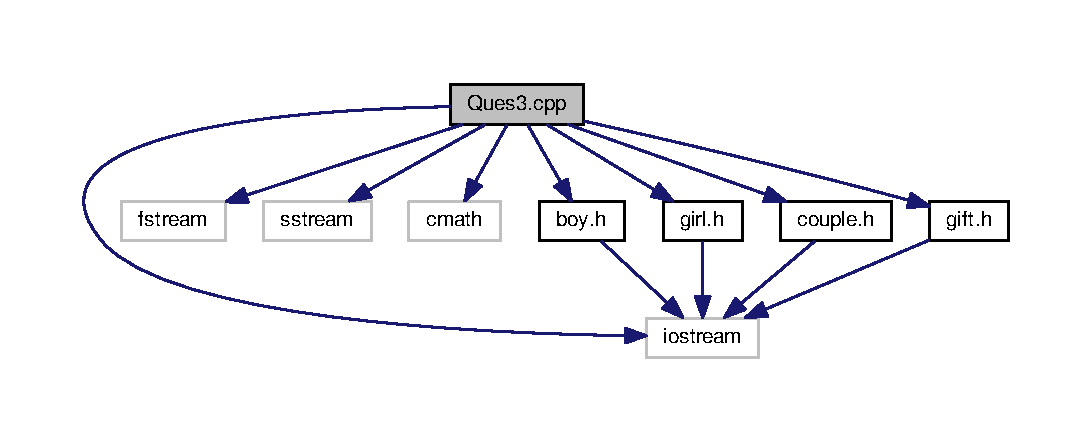
\includegraphics[width=350pt]{Ques3_8cpp__incl}
\end{center}
\end{figure}
\subsection*{Macros}
\begin{DoxyCompactItemize}
\item 
\#define \hyperlink{Ques3_8cpp_a111da81ae5883147168bbb8366377b10}{B}~9
\item 
\#define \hyperlink{Ques3_8cpp_aed9ea78689ecce0b7264c02c7f8a9a54}{G}~5
\item 
\#define \hyperlink{Ques3_8cpp_ac4cf4b2ab929bd23951a8676eeac086b}{C}~5
\item 
\#define \hyperlink{Ques3_8cpp_a5e0c07e523d4e77a2cafca06feb836f6}{Gf}~15
\item 
\#define \hyperlink{Ques3_8cpp_a97d832ae23af4f215e801e37e4f94254}{K}~2
\end{DoxyCompactItemize}
\subsection*{Functions}
\begin{DoxyCompactItemize}
\item 
void \hyperlink{Ques3_8cpp_ac70f752855ee1cf9ceaa2d749bbad17d}{swap} (\hyperlink{classGift}{Gift} \&a, \hyperlink{classGift}{Gift} \&b)
\item 
void \hyperlink{Ques3_8cpp_a9ed5e5ebda90f206f83cd424ebebe79d}{swapC} (\hyperlink{classCouple}{Couple} \&a, \hyperlink{classCouple}{Couple} \&b)
\item 
int \hyperlink{Ques3_8cpp_ae66f6b31b5ad750f1fe042a706a4e3d4}{main} ()
\end{DoxyCompactItemize}


\subsection{Macro Definition Documentation}
\index{Ques3.\+cpp@{Ques3.\+cpp}!B@{B}}
\index{B@{B}!Ques3.\+cpp@{Ques3.\+cpp}}
\subsubsection[{\texorpdfstring{B}{B}}]{\setlength{\rightskip}{0pt plus 5cm}\#define B~9}\hypertarget{Ques3_8cpp_a111da81ae5883147168bbb8366377b10}{}\label{Ques3_8cpp_a111da81ae5883147168bbb8366377b10}
\index{Ques3.\+cpp@{Ques3.\+cpp}!C@{C}}
\index{C@{C}!Ques3.\+cpp@{Ques3.\+cpp}}
\subsubsection[{\texorpdfstring{C}{C}}]{\setlength{\rightskip}{0pt plus 5cm}\#define C~5}\hypertarget{Ques3_8cpp_ac4cf4b2ab929bd23951a8676eeac086b}{}\label{Ques3_8cpp_ac4cf4b2ab929bd23951a8676eeac086b}
\index{Ques3.\+cpp@{Ques3.\+cpp}!G@{G}}
\index{G@{G}!Ques3.\+cpp@{Ques3.\+cpp}}
\subsubsection[{\texorpdfstring{G}{G}}]{\setlength{\rightskip}{0pt plus 5cm}\#define G~5}\hypertarget{Ques3_8cpp_aed9ea78689ecce0b7264c02c7f8a9a54}{}\label{Ques3_8cpp_aed9ea78689ecce0b7264c02c7f8a9a54}
\index{Ques3.\+cpp@{Ques3.\+cpp}!Gf@{Gf}}
\index{Gf@{Gf}!Ques3.\+cpp@{Ques3.\+cpp}}
\subsubsection[{\texorpdfstring{Gf}{Gf}}]{\setlength{\rightskip}{0pt plus 5cm}\#define Gf~15}\hypertarget{Ques3_8cpp_a5e0c07e523d4e77a2cafca06feb836f6}{}\label{Ques3_8cpp_a5e0c07e523d4e77a2cafca06feb836f6}
\index{Ques3.\+cpp@{Ques3.\+cpp}!K@{K}}
\index{K@{K}!Ques3.\+cpp@{Ques3.\+cpp}}
\subsubsection[{\texorpdfstring{K}{K}}]{\setlength{\rightskip}{0pt plus 5cm}\#define K~2}\hypertarget{Ques3_8cpp_a97d832ae23af4f215e801e37e4f94254}{}\label{Ques3_8cpp_a97d832ae23af4f215e801e37e4f94254}


\subsection{Function Documentation}
\index{Ques3.\+cpp@{Ques3.\+cpp}!main@{main}}
\index{main@{main}!Ques3.\+cpp@{Ques3.\+cpp}}
\subsubsection[{\texorpdfstring{main()}{main()}}]{\setlength{\rightskip}{0pt plus 5cm}int main (
\begin{DoxyParamCaption}
{}
\end{DoxyParamCaption}
)}\hypertarget{Ques3_8cpp_ae66f6b31b5ad750f1fe042a706a4e3d4}{}\label{Ques3_8cpp_ae66f6b31b5ad750f1fe042a706a4e3d4}
taking input from boy.\+dat

taking input from girl.\+dat

taking input gift.\+dat

forming couples

printing couples

sorting gifts

Assigning gifts to couples

printing assigned gifts

calculating compatibility

calculating happiness

sorting couples according to compatibility

sorting couples according to happiness
\begin{DoxyCode}
34 \{
35     \hyperlink{classBoy}{Boy} boys[\hyperlink{Ques3_8cpp_a111da81ae5883147168bbb8366377b10}{B}];
36     \hyperlink{classGirl}{Girl} girls[\hyperlink{Ques3_8cpp_aed9ea78689ecce0b7264c02c7f8a9a54}{G}];
37     \hyperlink{classCouple}{Couple} couples[\hyperlink{Ques3_8cpp_ac4cf4b2ab929bd23951a8676eeac086b}{C}];
38     \hyperlink{classGift}{Gift} gifts[\hyperlink{Ques3_8cpp_a5e0c07e523d4e77a2cafca06feb836f6}{Gf}];
39     
40     \textcolor{keywordtype}{string} line;
41     \textcolor{keywordtype}{int} c = 0, x = 0;
42 
43     ofstream logFile;
44     logFile.open(\textcolor{stringliteral}{"logFile3.dat"});
45 
46 
50     ifstream boyInp(\textcolor{stringliteral}{"boy.dat"});
51     \textcolor{keywordflow}{while}(getline(boyInp,line)) \{
52         \textcolor{keywordflow}{if}(c++ == 0) \textcolor{keywordflow}{continue};
53         istringstream iss(line);
54         \textcolor{keywordtype}{string} name;
55         \textcolor{keywordtype}{int} a,i,b,t,s;
56         \textcolor{keywordtype}{char} ty;
57         \textcolor{keywordflow}{if}((iss>>name>>a>>i>>b>>t>>s>>ty))\{
58             boys[x++].\hyperlink{classBoy_a6ac70867d517f6b429ce67c8eb2915ed}{setDetails}(name,a,i,b,t,s,ty);
59         \} \textcolor{keywordflow}{else} \{
60             \textcolor{keywordflow}{break};
61         \}
62     \}
63 
64     c = 0;
65     x = 0;
66 
70     ifstream girlInp(\textcolor{stringliteral}{"girl.dat"});
71     \textcolor{keywordflow}{while}(getline(girlInp,line)) \{
72         \textcolor{keywordflow}{if}(c++ == 0) \textcolor{keywordflow}{continue};
73         istringstream iss(line);
74         \textcolor{keywordtype}{string} name;
75         \textcolor{keywordtype}{int} a,i,m,s;
76         \textcolor{keywordtype}{char} ty,cr;
77         \textcolor{keywordflow}{if}((iss>>name>>a>>i>>m>>cr>>s>>ty))\{
78             girls[x++].\hyperlink{classGirl_a4bff314dba17278eb1093b15f7be80bd}{setDetails}(name,a,i,m,ty,s,cr);
79         \} \textcolor{keywordflow}{else} \{
80             \textcolor{keywordflow}{break};
81         \}
82     \}
83 
84     c = 0;
85     x = 0;
89     ifstream giftInp(\textcolor{stringliteral}{"gift.dat"});
90     \textcolor{keywordflow}{while}(getline(giftInp,line)) \{
91         \textcolor{keywordflow}{if}(c++ == 0) \textcolor{keywordflow}{continue};
92         istringstream iss(line);
93         \textcolor{keywordtype}{int} id,p,v;
94         \textcolor{keywordtype}{char} ty;
95         \textcolor{keywordflow}{if}((iss>>\textcolor{keywordtype}{id}>>p>>ty>>v))\{
96             gifts[x++].\hyperlink{classGift_abc74fbed8b31b5bb7745b3e0c934da9e}{setDetail}(\textcolor{keywordtype}{id},p,ty,0);
97         \} \textcolor{keywordflow}{else} \{
98             \textcolor{keywordflow}{break};
99         \}
100     \}
101     
102     c = 0;
106     \textcolor{keywordflow}{for}(\textcolor{keywordtype}{int} i = 0 ; i < \hyperlink{Ques3_8cpp_aed9ea78689ecce0b7264c02c7f8a9a54}{G}; i++) \{
107         \textcolor{keywordflow}{if}(girls[i].getCriterion() == \textcolor{charliteral}{'A'}) \{
108             \textcolor{keywordtype}{int} max= -99;
109             \textcolor{keywordtype}{int} ind = -1;
110             \textcolor{keywordflow}{for}(\textcolor{keywordtype}{int} j = 0; j < \hyperlink{Ques3_8cpp_a111da81ae5883147168bbb8366377b10}{B}; j++) \{
111                 \textcolor{keywordflow}{if}(boys[j].getAttractiveness() > max && boys[j].getStatus() == 0) \{
112                     \textcolor{keywordflow}{if}(boys[j].getBudget() > girls[i].getMaintenance()) \{
113                         \textcolor{keywordflow}{if}(girls[i].getAttractiveness() > boys[j].getThreshold()) \{
114                             max = boys[j].\hyperlink{classBoy_a814ef4919f2ac86c6ee70f9698afad3d}{getAttractiveness}();
115                             ind = j;
116                         \}
117                     \}
118                 \}
119             \}
120         
121             \textcolor{keywordflow}{if}(ind != -1) \{
122                 boys[ind].\hyperlink{classBoy_a3d29dcc4137fbfc0306cbd7df82781c3}{setStatus}(1);
123                 girls[i].\hyperlink{classGirl_a201527323b3fabac4b089f003b8fcc4a}{setStatus}(1);
124                 couples[c++].\hyperlink{classCouple_a0057d3dfd3939a156cd99f6c5cf32279}{setDetails}(boys[ind].getName(),girls[i].getname()) ; 
125             \}       
126         \} \textcolor{keywordflow}{else} \textcolor{keywordflow}{if}(girls[i].getCriterion() == \textcolor{charliteral}{'I'}) \{
127             \textcolor{keywordtype}{int} max= -99;
128                         \textcolor{keywordtype}{int} ind = -1;
129                         \textcolor{keywordflow}{for}(\textcolor{keywordtype}{int} j = 0; j < \hyperlink{Ques3_8cpp_a111da81ae5883147168bbb8366377b10}{B}; j++) \{
130                                 \textcolor{keywordflow}{if}(boys[j].getIntelligence() > max && boys[j].getStatus() == 0) \{
131                                         \textcolor{keywordflow}{if}(boys[j].getBudget() > girls[i].getMaintenance()) \{
132                                                 \textcolor{keywordflow}{if}(girls[i].getAttractiveness() > boys[j].getThreshold()) \{
133                                                         max = boys[j].
      \hyperlink{classBoy_ad52c9e04ab591f3909d2342d6cae0168}{getIntelligence}();
134                                                         ind = j;
135                                                 \}
136                                         \}
137                                 \}
138                         \}
139                           
140                         \textcolor{keywordflow}{if}(ind != -1) \{
141                                 boys[ind].\hyperlink{classBoy_a3d29dcc4137fbfc0306cbd7df82781c3}{setStatus}(1);
142                                 girls[i].\hyperlink{classGirl_a201527323b3fabac4b089f003b8fcc4a}{setStatus}(1);
143                                 couples[c++].\hyperlink{classCouple_a0057d3dfd3939a156cd99f6c5cf32279}{setDetails}(boys[ind].getName(),girls[i].getname()) ;
144                         \}
145 
146         \} \textcolor{keywordflow}{else} \{
147             \textcolor{keywordtype}{int} max= -99;
148                         \textcolor{keywordtype}{int} ind = -1;
149                         \textcolor{keywordflow}{for}(\textcolor{keywordtype}{int} j = 0; j < \hyperlink{Ques3_8cpp_a111da81ae5883147168bbb8366377b10}{B}; j++) \{
150                                 \textcolor{keywordflow}{if}(boys[j].getBudget() > max && boys[j].getStatus() == 0) \{
151                                         \textcolor{keywordflow}{if}(boys[j].getBudget() > girls[i].getMaintenance()) \{
152                                                 \textcolor{keywordflow}{if}(girls[i].getAttractiveness() > boys[j].getThreshold()) \{
153                                                         max = boys[j].\hyperlink{classBoy_a05c48b12091ebcad44ba86ba88514ac5}{getBudget}();
154                                                         ind = j;
155                                                 \}
156                                         \}
157                                 \}
158                         \}
159                           
160                         \textcolor{keywordflow}{if}(ind != -1) \{
161                                 boys[ind].\hyperlink{classBoy_a3d29dcc4137fbfc0306cbd7df82781c3}{setStatus}(1);
162                                 girls[i].\hyperlink{classGirl_a201527323b3fabac4b089f003b8fcc4a}{setStatus}(1);
163                                 couples[c++].\hyperlink{classCouple_a0057d3dfd3939a156cd99f6c5cf32279}{setDetails}(boys[ind].getName(),girls[i].getname()) ;
164                         \}
165             
166         \}
167     \}
168 logFile<<\textcolor{stringliteral}{"-----------------COUPLES-------------------\(\backslash\)n\(\backslash\)n"};
172 
173     \textcolor{keywordflow}{for}(\textcolor{keywordtype}{int} i = 0 ;i < \hyperlink{Ques3_8cpp_ac4cf4b2ab929bd23951a8676eeac086b}{C}; i++) \{
174         logFile<<\textcolor{stringliteral}{"Boy b"}<<couples[i].\hyperlink{classCouple_a092cbc580ea255febc3eb211c5f56512}{getBoy}()<<\textcolor{stringliteral}{" and Girl g"}<<couples[i].
      \hyperlink{classCouple_a653983df7e331c0534ae2ce42e9856c5}{getGirl}()<<\textcolor{stringliteral}{"\(\backslash\)n"};
175         
176     \}
177 
181     \textcolor{keywordflow}{for}(\textcolor{keywordtype}{int} i = 0  ; i< \hyperlink{Ques3_8cpp_a5e0c07e523d4e77a2cafca06feb836f6}{Gf}-1; i++) \{
182         \textcolor{keywordflow}{for}(\textcolor{keywordtype}{int} j = i+1; j < \hyperlink{Ques3_8cpp_a5e0c07e523d4e77a2cafca06feb836f6}{Gf}; j++) \{
183             \textcolor{keywordflow}{if}(gifts[j].getprice() < gifts[i].getprice()) \{
184                 \hyperlink{Ques3_8cpp_ac70f752855ee1cf9ceaa2d749bbad17d}{swap}(gifts[j],gifts[i]);
185             \}
186         \}
187     \}
188 
192     \textcolor{keywordflow}{for}(\textcolor{keywordtype}{int} i  = 0 ;i < \hyperlink{Ques3_8cpp_ac4cf4b2ab929bd23951a8676eeac086b}{C}; i++) \{
193         \textcolor{keywordtype}{int} boy = couples[i].\hyperlink{classCouple_a092cbc580ea255febc3eb211c5f56512}{getBoy}()[0] - 48;
194         \textcolor{keywordtype}{int} girl = couples[i].\hyperlink{classCouple_a653983df7e331c0534ae2ce42e9856c5}{getGirl}()[0] - 48;
195         \textcolor{keywordtype}{int} mc = girls[girl-1].\hyperlink{classGirl_a6192affb0721b385d2c5d83a011a869e}{getMaintenance}();
196         \textcolor{keywordtype}{int} bud = boys[boy-1].\hyperlink{classBoy_a05c48b12091ebcad44ba86ba88514ac5}{getBudget}();
197         \textcolor{keywordtype}{int} x = bud - mc;
198         \textcolor{keywordtype}{char} bt = boys[boy-1].\hyperlink{classBoy_a01accc077c0824f7e28cfe391f7851c7}{getType}(); 
199     
200         \textcolor{keywordflow}{if}(bt == \textcolor{charliteral}{'M'}) \{
201             \textcolor{keywordflow}{for}(\textcolor{keywordtype}{int} j = 0 ; j < \hyperlink{Ques3_8cpp_a5e0c07e523d4e77a2cafca06feb836f6}{Gf}; j++) \{
202                 
203                 \textcolor{keywordflow}{if}(gifts[j].getprice() <= mc && gifts[j].getStatus() == 0) \{
204                     couples[i].\hyperlink{classCouple_a1a621700c479fd808b0caf034f4bd0f5}{setGifts}(j+1);
205                     gifts[j].\hyperlink{classGift_a8c8a8be33c3abe17bbe4b8da9ac084d6}{setStatus}(1);
206                     mc = mc - gifts[j].\hyperlink{classGift_aa36f2b437e93ede1d2569e489b493441}{getprice}();
207                 \} \textcolor{keywordflow}{else} \textcolor{keywordflow}{if}( gifts[j].getprice() <= x +mc ) \{
208                     \textcolor{keywordflow}{if}( gifts[j].getStatus() == 0)  \{               
209                         couples[i].\hyperlink{classCouple_a1a621700c479fd808b0caf034f4bd0f5}{setGifts}(j+1);
210                         gifts[j].\hyperlink{classGift_a8c8a8be33c3abe17bbe4b8da9ac084d6}{setStatus}(1);
211                         \textcolor{keywordflow}{break};
212                     \}
213                 \} \textcolor{keywordflow}{else} \{
214                     \textcolor{keywordflow}{break};
215                 \}
216             \} 
217         \} \textcolor{keywordflow}{else}  \textcolor{keywordflow}{if}(bt == \textcolor{charliteral}{'N'}) \{
218             \textcolor{keywordflow}{for}(\textcolor{keywordtype}{int} j = Gf-1 ; j >= 0; j--) \{
219                 \textcolor{keywordflow}{if}(gifts[j].getprice() <= bud && gifts[j].getStatus() == 0) \{
220                     couples[i].\hyperlink{classCouple_a1a621700c479fd808b0caf034f4bd0f5}{setGifts}(j+1);
221                     gifts[j].\hyperlink{classGift_a8c8a8be33c3abe17bbe4b8da9ac084d6}{setStatus}(1);
222                     bud = bud- gifts[j].\hyperlink{classGift_aa36f2b437e93ede1d2569e489b493441}{getprice}();
223                 \}
224             \}
225         \} \textcolor{keywordflow}{else} \{
226             \textcolor{keywordflow}{for}(\textcolor{keywordtype}{int} j = 0 ; j < \hyperlink{Ques3_8cpp_a5e0c07e523d4e77a2cafca06feb836f6}{Gf}; j++) \{
227                 \textcolor{keywordflow}{if}(gifts[j].getprice() <= mc && gifts[j].getStatus() == 0) \{
228                     couples[i].\hyperlink{classCouple_a1a621700c479fd808b0caf034f4bd0f5}{setGifts}(j+1);
229                     gifts[j].\hyperlink{classGift_a8c8a8be33c3abe17bbe4b8da9ac084d6}{setStatus}(1);
230                     mc = mc - gifts[j].\hyperlink{classGift_aa36f2b437e93ede1d2569e489b493441}{getprice}();
231                 \}\textcolor{keywordflow}{else} \textcolor{keywordflow}{if}(gifts[j].getprice() <= x +mc) \{
232                     \textcolor{keywordflow}{if}( gifts[j].getStatus() == 0)  \{               
233                         couples[i].\hyperlink{classCouple_a1a621700c479fd808b0caf034f4bd0f5}{setGifts}(j+1);
234                         gifts[j].\hyperlink{classGift_a8c8a8be33c3abe17bbe4b8da9ac084d6}{setStatus}(1);
235                         \textcolor{keywordflow}{break};
236                     \}
237                 \} \textcolor{keywordflow}{else} \{
238                     \textcolor{keywordflow}{break};
239                 \}
240             \}
241         \}
242     \}
243     
247     logFile<<\textcolor{stringliteral}{"\(\backslash\)n\(\backslash\)n-----------------GIFTS ALLOCATION-------------------\(\backslash\)n\(\backslash\)n"};
248 
249     \textcolor{keywordflow}{for}(\textcolor{keywordtype}{int} i = 0 ;i < \hyperlink{Ques3_8cpp_ac4cf4b2ab929bd23951a8676eeac086b}{C}; i++) \{
250         logFile<<\textcolor{stringliteral}{"Boy b"}<<couples[i].\hyperlink{classCouple_a092cbc580ea255febc3eb211c5f56512}{getBoy}()<<\textcolor{stringliteral}{" gives Girl g"}<<couples[i].
      \hyperlink{classCouple_a653983df7e331c0534ae2ce42e9856c5}{getGirl}()<<\textcolor{stringliteral}{" the following Gifts\(\backslash\)n"};
251         
252         \textcolor{keywordtype}{int} * arr = couples[i].\hyperlink{classCouple_a80cef2647acb3903936372a0d70cf9cc}{getGifts}();
253         \textcolor{keywordflow}{for}(\textcolor{keywordtype}{int} j = 0; j < couples[i].\hyperlink{classCouple_a05a3bbd0d8d6b149ae04f5306acd4439}{getNum}(); j++) \{
254             logFile<<\textcolor{stringliteral}{"G"}<<gifts[arr[j]-1].\hyperlink{classGift_a5b276dda8fab4a4e2618ba82fc8cd787}{getId}()<<\textcolor{stringliteral}{" of worth Rs "}<<gifts[arr[j]-1].
      \hyperlink{classGift_aa36f2b437e93ede1d2569e489b493441}{getprice}()<<\textcolor{stringliteral}{"\(\backslash\)n"};
255         \}
256         logFile<<endl;
257     \}
258 
259 
263     \textcolor{keywordflow}{for}(\textcolor{keywordtype}{int} i = 0 ; i < \hyperlink{Ques3_8cpp_ac4cf4b2ab929bd23951a8676eeac086b}{C}; i++) \{
264         \textcolor{keywordtype}{int} boy = couples[i].\hyperlink{classCouple_a092cbc580ea255febc3eb211c5f56512}{getBoy}()[0] - 48;
265         \textcolor{keywordtype}{int} girl = couples[i].\hyperlink{classCouple_a653983df7e331c0534ae2ce42e9856c5}{getGirl}()[0] - 48;
266 
267         \textcolor{keywordtype}{int} mc = girls[girl-1].\hyperlink{classGirl_a6192affb0721b385d2c5d83a011a869e}{getMaintenance}();
268         \textcolor{keywordtype}{int} bud = boys[boy-1].\hyperlink{classBoy_a05c48b12091ebcad44ba86ba88514ac5}{getBudget}();
269         \textcolor{keywordtype}{int} x1 = bud - mc;
270 
271         \textcolor{keywordtype}{int} ag = girls[girl-1].\hyperlink{classGirl_a04cfe3e0c21240f92c19152630a40252}{getAttractiveness}();
272         \textcolor{keywordtype}{int} ab = boys[boy-1].\hyperlink{classBoy_a814ef4919f2ac86c6ee70f9698afad3d}{getAttractiveness}();
273         \textcolor{keywordtype}{int} x2 = abs(ag-ab);                
274 
275         \textcolor{keywordtype}{int} ib = boys[boy-1].\hyperlink{classBoy_ad52c9e04ab591f3909d2342d6cae0168}{getIntelligence}();
276         \textcolor{keywordtype}{int} ig = girls[girl-1].\hyperlink{classGirl_afe73c4c4f180aa8f5e0bc4f87455ec0b}{getIntelligence}();
277         \textcolor{keywordtype}{int} x3 = abs(ib- ig);
278 
279         couples[i].\hyperlink{classCouple_a4fe1bbdbf59458c1a903569b6f2edca3}{setCompatibility}(x1 + x2 + x3);      
280     \}
281 
285     \textcolor{keywordflow}{for}(\textcolor{keywordtype}{int} i = 0; i < \hyperlink{Ques3_8cpp_ac4cf4b2ab929bd23951a8676eeac086b}{C}; i++) \{
286         \textcolor{keywordtype}{int} boy = couples[i].\hyperlink{classCouple_a092cbc580ea255febc3eb211c5f56512}{getBoy}()[0] - 48;
287         \textcolor{keywordtype}{int} girl = couples[i].\hyperlink{classCouple_a653983df7e331c0534ae2ce42e9856c5}{getGirl}()[0] - 48;
288 
289         \textcolor{keywordtype}{int} mc = girls[girl-1].\hyperlink{classGirl_a6192affb0721b385d2c5d83a011a869e}{getMaintenance}();
290         \textcolor{keywordtype}{int} bud = boys[boy-1].\hyperlink{classBoy_a05c48b12091ebcad44ba86ba88514ac5}{getBudget}();
291         \textcolor{keywordtype}{int} x1 = bud - mc;
292 
293         \textcolor{keywordtype}{char} bt = boys[boy-1].\hyperlink{classBoy_a01accc077c0824f7e28cfe391f7851c7}{getType}();
294         \textcolor{keywordtype}{char} gt = girls[girl-1].\hyperlink{classGirl_af26252dbf5784c2c79744dd4652a3bf2}{getType}();
295         
296         \textcolor{keywordtype}{int} hb = 0;
297         \textcolor{keywordtype}{int} hg = 0;
298 
299         \textcolor{keywordtype}{int} total = 0;
300     
301         
302         \textcolor{keywordtype}{int} * arr = couples[i].\hyperlink{classCouple_a80cef2647acb3903936372a0d70cf9cc}{getGifts}();
303         \textcolor{keywordflow}{for}(\textcolor{keywordtype}{int} j = 0 ; j < couples[i].\hyperlink{classCouple_a05a3bbd0d8d6b149ae04f5306acd4439}{getNum}(); j++) \{
304             total += gifts[arr[j]-1].\hyperlink{classGift_aa36f2b437e93ede1d2569e489b493441}{getprice}();
305         \}
306     
307         \textcolor{keywordflow}{if}(bt == \textcolor{charliteral}{'M'}) \{
308             hb = bud-total;
309         \} \textcolor{keywordflow}{else} \textcolor{keywordflow}{if}(bt == \textcolor{charliteral}{'N'}) \{
310             hb = hg;
311         \} \textcolor{keywordflow}{else} \{
312             hb = girls[girl-1].\hyperlink{classGirl_afe73c4c4f180aa8f5e0bc4f87455ec0b}{getIntelligence}();
313         \}
314 
315         \textcolor{keywordflow}{if}(gt == \textcolor{charliteral}{'C'}) \{
316             hg = log(abs(mc-total));
317         \} \textcolor{keywordflow}{else} \textcolor{keywordflow}{if}(gt == \textcolor{charliteral}{'N'}) \{
318             hg = abs(mc-total);
319         \} \textcolor{keywordflow}{else} \{
320             hg = exp(abs(mc-total));
321         \}
322         couples[i].\hyperlink{classCouple_a19afd8575f26caa557115a106b6a4928}{setHappiness}(hb + abs(hg));
323         
324     \}
325 
326     
330     \textcolor{keywordflow}{for}(\textcolor{keywordtype}{int} i = 0  ; i< C-1; i++) \{
331         \textcolor{keywordflow}{for}(\textcolor{keywordtype}{int} j = i+1; j < \hyperlink{Ques3_8cpp_ac4cf4b2ab929bd23951a8676eeac086b}{C}; j++) \{
332             \textcolor{keywordflow}{if}(couples[i].getCompatibility() > couples[j].getCompatibility()) \{
333                 \hyperlink{Ques3_8cpp_a9ed5e5ebda90f206f83cd424ebebe79d}{swapC}(couples[i],couples[j]);
334             \}   
335         \}
336     \}
337 
338     logFile<<\textcolor{stringliteral}{"\(\backslash\)n------------------Most Compatible---------------------\(\backslash\)n\(\backslash\)n"};
339     \textcolor{keywordflow}{for}(\textcolor{keywordtype}{int} i = C-1 ;i >= C-\hyperlink{Ques3_8cpp_a97d832ae23af4f215e801e37e4f94254}{K}; i--) \{
340         logFile<<\textcolor{stringliteral}{"Boy b"}<<couples[i].\hyperlink{classCouple_a092cbc580ea255febc3eb211c5f56512}{getBoy}()<<\textcolor{stringliteral}{" and Girl g"}<<couples[i].
      \hyperlink{classCouple_a653983df7e331c0534ae2ce42e9856c5}{getGirl}()<<\textcolor{stringliteral}{"\(\backslash\)n"};;
341     \}
342 
343 \textcolor{keywordflow}{for}(\textcolor{keywordtype}{int} i = 0  ; i< C-1; i++) \{
347         \textcolor{keywordflow}{for}(\textcolor{keywordtype}{int} j = i+1; j < \hyperlink{Ques3_8cpp_ac4cf4b2ab929bd23951a8676eeac086b}{C}; j++) \{
348             \textcolor{keywordflow}{if}(couples[i].getHappiness() > couples[j].getHappiness()) \{
349                 \hyperlink{Ques3_8cpp_a9ed5e5ebda90f206f83cd424ebebe79d}{swapC}(couples[i],couples[j]);
350             \}   
351         \}
352     \}
353     
354     logFile<<\textcolor{stringliteral}{"\(\backslash\)n---------------------Most Happy------------------------\(\backslash\)n\(\backslash\)n"};
355     \textcolor{keywordflow}{for}(\textcolor{keywordtype}{int} i = C-1 ;i >= C-\hyperlink{Ques3_8cpp_a97d832ae23af4f215e801e37e4f94254}{K}; i--) \{
356         logFile<<\textcolor{stringliteral}{"Boy b"}<<couples[i].\hyperlink{classCouple_a092cbc580ea255febc3eb211c5f56512}{getBoy}()<<\textcolor{stringliteral}{" and Girl g"}<<couples[i].
      \hyperlink{classCouple_a653983df7e331c0534ae2ce42e9856c5}{getGirl}()<<\textcolor{stringliteral}{"\(\backslash\)n"};
357     \}
358 
359     
360 
361     logFile.close();
362 \}
\end{DoxyCode}
\index{Ques3.\+cpp@{Ques3.\+cpp}!swap@{swap}}
\index{swap@{swap}!Ques3.\+cpp@{Ques3.\+cpp}}
\subsubsection[{\texorpdfstring{swap(\+Gift \&a, Gift \&b)}{swap(Gift &a, Gift &b)}}]{\setlength{\rightskip}{0pt plus 5cm}void swap (
\begin{DoxyParamCaption}
\item[{{\bf Gift} \&}]{a, }
\item[{{\bf Gift} \&}]{b}
\end{DoxyParamCaption}
)}\hypertarget{Ques3_8cpp_ac70f752855ee1cf9ceaa2d749bbad17d}{}\label{Ques3_8cpp_ac70f752855ee1cf9ceaa2d749bbad17d}

\begin{DoxyCode}
20 \{
21     \hyperlink{classGift}{Gift} temp = a;
22     a = b;
23     b = temp;
24 \}
\end{DoxyCode}
\index{Ques3.\+cpp@{Ques3.\+cpp}!swapC@{swapC}}
\index{swapC@{swapC}!Ques3.\+cpp@{Ques3.\+cpp}}
\subsubsection[{\texorpdfstring{swap\+C(\+Couple \&a, Couple \&b)}{swapC(Couple &a, Couple &b)}}]{\setlength{\rightskip}{0pt plus 5cm}void swapC (
\begin{DoxyParamCaption}
\item[{{\bf Couple} \&}]{a, }
\item[{{\bf Couple} \&}]{b}
\end{DoxyParamCaption}
)}\hypertarget{Ques3_8cpp_a9ed5e5ebda90f206f83cd424ebebe79d}{}\label{Ques3_8cpp_a9ed5e5ebda90f206f83cd424ebebe79d}

\begin{DoxyCode}
27 \{
28     \hyperlink{classCouple}{Couple} temp = a;
29     a = b;
30     b = temp;
31 \}
\end{DoxyCode}

\hypertarget{Ques4_8cpp}{}\section{Ques4.\+cpp File Reference}
\label{Ques4_8cpp}\index{Ques4.\+cpp@{Ques4.\+cpp}}
{\ttfamily \#include $<$iostream$>$}\\*
{\ttfamily \#include $<$fstream$>$}\\*
{\ttfamily \#include $<$sstream$>$}\\*
{\ttfamily \#include $<$cmath$>$}\\*
{\ttfamily \#include \char`\"{}boy.\+h\char`\"{}}\\*
{\ttfamily \#include \char`\"{}girl.\+h\char`\"{}}\\*
{\ttfamily \#include \char`\"{}couple.\+h\char`\"{}}\\*
{\ttfamily \#include \char`\"{}gift.\+h\char`\"{}}\\*
Include dependency graph for Ques4.\+cpp\+:
\nopagebreak
\begin{figure}[H]
\begin{center}
\leavevmode
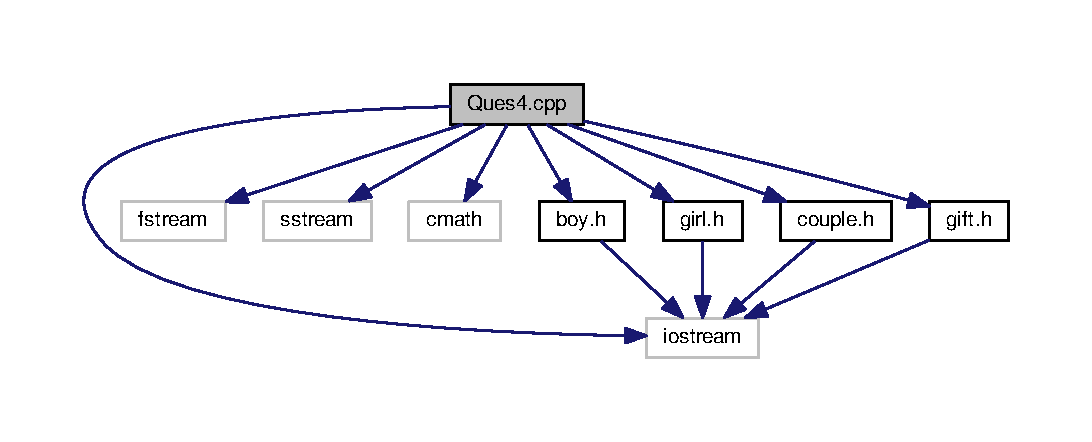
\includegraphics[width=350pt]{Ques4_8cpp__incl}
\end{center}
\end{figure}
\subsection*{Macros}
\begin{DoxyCompactItemize}
\item 
\#define \hyperlink{Ques4_8cpp_a111da81ae5883147168bbb8366377b10}{B}~9
\item 
\#define \hyperlink{Ques4_8cpp_aed9ea78689ecce0b7264c02c7f8a9a54}{G}~5
\item 
\#define \hyperlink{Ques4_8cpp_ac4cf4b2ab929bd23951a8676eeac086b}{C}~5
\item 
\#define \hyperlink{Ques4_8cpp_a5e0c07e523d4e77a2cafca06feb836f6}{Gf}~15
\item 
\#define \hyperlink{Ques4_8cpp_a97d832ae23af4f215e801e37e4f94254}{K}~2
\end{DoxyCompactItemize}
\subsection*{Functions}
\begin{DoxyCompactItemize}
\item 
void \hyperlink{Ques4_8cpp_ac70f752855ee1cf9ceaa2d749bbad17d}{swap} (\hyperlink{classGift}{Gift} \&a, \hyperlink{classGift}{Gift} \&b)
\item 
void \hyperlink{Ques4_8cpp_a9ed5e5ebda90f206f83cd424ebebe79d}{swapC} (\hyperlink{classCouple}{Couple} \&a, \hyperlink{classCouple}{Couple} \&b)
\item 
int \hyperlink{Ques4_8cpp_ae66f6b31b5ad750f1fe042a706a4e3d4}{main} ()
\end{DoxyCompactItemize}


\subsection{Macro Definition Documentation}
\index{Ques4.\+cpp@{Ques4.\+cpp}!B@{B}}
\index{B@{B}!Ques4.\+cpp@{Ques4.\+cpp}}
\subsubsection[{\texorpdfstring{B}{B}}]{\setlength{\rightskip}{0pt plus 5cm}\#define B~9}\hypertarget{Ques4_8cpp_a111da81ae5883147168bbb8366377b10}{}\label{Ques4_8cpp_a111da81ae5883147168bbb8366377b10}
\index{Ques4.\+cpp@{Ques4.\+cpp}!C@{C}}
\index{C@{C}!Ques4.\+cpp@{Ques4.\+cpp}}
\subsubsection[{\texorpdfstring{C}{C}}]{\setlength{\rightskip}{0pt plus 5cm}\#define C~5}\hypertarget{Ques4_8cpp_ac4cf4b2ab929bd23951a8676eeac086b}{}\label{Ques4_8cpp_ac4cf4b2ab929bd23951a8676eeac086b}
\index{Ques4.\+cpp@{Ques4.\+cpp}!G@{G}}
\index{G@{G}!Ques4.\+cpp@{Ques4.\+cpp}}
\subsubsection[{\texorpdfstring{G}{G}}]{\setlength{\rightskip}{0pt plus 5cm}\#define G~5}\hypertarget{Ques4_8cpp_aed9ea78689ecce0b7264c02c7f8a9a54}{}\label{Ques4_8cpp_aed9ea78689ecce0b7264c02c7f8a9a54}
\index{Ques4.\+cpp@{Ques4.\+cpp}!Gf@{Gf}}
\index{Gf@{Gf}!Ques4.\+cpp@{Ques4.\+cpp}}
\subsubsection[{\texorpdfstring{Gf}{Gf}}]{\setlength{\rightskip}{0pt plus 5cm}\#define Gf~15}\hypertarget{Ques4_8cpp_a5e0c07e523d4e77a2cafca06feb836f6}{}\label{Ques4_8cpp_a5e0c07e523d4e77a2cafca06feb836f6}
\index{Ques4.\+cpp@{Ques4.\+cpp}!K@{K}}
\index{K@{K}!Ques4.\+cpp@{Ques4.\+cpp}}
\subsubsection[{\texorpdfstring{K}{K}}]{\setlength{\rightskip}{0pt plus 5cm}\#define K~2}\hypertarget{Ques4_8cpp_a97d832ae23af4f215e801e37e4f94254}{}\label{Ques4_8cpp_a97d832ae23af4f215e801e37e4f94254}


\subsection{Function Documentation}
\index{Ques4.\+cpp@{Ques4.\+cpp}!main@{main}}
\index{main@{main}!Ques4.\+cpp@{Ques4.\+cpp}}
\subsubsection[{\texorpdfstring{main()}{main()}}]{\setlength{\rightskip}{0pt plus 5cm}int main (
\begin{DoxyParamCaption}
{}
\end{DoxyParamCaption}
)}\hypertarget{Ques4_8cpp_ae66f6b31b5ad750f1fe042a706a4e3d4}{}\label{Ques4_8cpp_ae66f6b31b5ad750f1fe042a706a4e3d4}
taking input from boy.\+dat

taking input from girl.\+dat

taking input gift.\+dat

forming couples

printing couples

sorting gifts

Assigning gifts to couples

calculating happiness

sorting couples according to happiness
\begin{DoxyCode}
36 \{
37     \hyperlink{classBoy}{Boy} boys[\hyperlink{Ques4_8cpp_a111da81ae5883147168bbb8366377b10}{B}];
38     \hyperlink{classGirl}{Girl} girls[\hyperlink{Ques4_8cpp_aed9ea78689ecce0b7264c02c7f8a9a54}{G}];
39     \hyperlink{classCouple}{Couple} couples[\hyperlink{Ques4_8cpp_ac4cf4b2ab929bd23951a8676eeac086b}{C}];
40     \hyperlink{classGift}{Gift} gifts[\hyperlink{Ques4_8cpp_a5e0c07e523d4e77a2cafca06feb836f6}{Gf}];
41     
42     \textcolor{keywordtype}{string} line;
43     \textcolor{keywordtype}{int} c = 0, x = 0;
44 
45     ofstream logFile;
46     logFile.open(\textcolor{stringliteral}{"logFile4.dat"});
47 
48 
52     ifstream boyInp(\textcolor{stringliteral}{"boy.dat"});
53     \textcolor{keywordflow}{while}(getline(boyInp,line)) \{
54         \textcolor{keywordflow}{if}(c++ == 0) \textcolor{keywordflow}{continue};
55         istringstream iss(line);
56         \textcolor{keywordtype}{string} name;
57         \textcolor{keywordtype}{int} a,i,b,t,s;
58         \textcolor{keywordtype}{char} ty;
59         \textcolor{keywordflow}{if}((iss>>name>>a>>i>>b>>t>>s>>ty))\{
60             boys[x++].\hyperlink{classBoy_a6ac70867d517f6b429ce67c8eb2915ed}{setDetails}(name,a,i,b,t,s,ty);
61         \} \textcolor{keywordflow}{else} \{
62             \textcolor{keywordflow}{break};
63         \}
64     \}
65 
66     c = 0;
67     x = 0;
71     ifstream girlInp(\textcolor{stringliteral}{"girl.dat"});
72     \textcolor{keywordflow}{while}(getline(girlInp,line)) \{
73         \textcolor{keywordflow}{if}(c++ == 0) \textcolor{keywordflow}{continue};
74         istringstream iss(line);
75         \textcolor{keywordtype}{string} name;
76         \textcolor{keywordtype}{int} a,i,m,s;
77         \textcolor{keywordtype}{char} ty,cr;
78         \textcolor{keywordflow}{if}((iss>>name>>a>>i>>m>>cr>>s>>ty))\{
79             girls[x++].\hyperlink{classGirl_a4bff314dba17278eb1093b15f7be80bd}{setDetails}(name,a,i,m,ty,s,cr);
80         \} \textcolor{keywordflow}{else} \{
81             \textcolor{keywordflow}{break};
82         \}
83     \}
84 
85     c = 0;
86     x = 0;
90     ifstream giftInp(\textcolor{stringliteral}{"gift.dat"});
91     \textcolor{keywordflow}{while}(getline(giftInp,line)) \{
92         \textcolor{keywordflow}{if}(c++ == 0) \textcolor{keywordflow}{continue};
93         istringstream iss(line);
94         \textcolor{keywordtype}{int} id,p,v;
95         \textcolor{keywordtype}{char} ty;
96         \textcolor{keywordflow}{if}((iss>>\textcolor{keywordtype}{id}>>p>>ty>>v))\{
97             gifts[x++].\hyperlink{classGift_abc74fbed8b31b5bb7745b3e0c934da9e}{setDetail}(\textcolor{keywordtype}{id},p,ty,0);
98         \} \textcolor{keywordflow}{else} \{
99             \textcolor{keywordflow}{break};
100         \}
101     \}
102     
103     c = 0;
107     \textcolor{keywordflow}{for}(\textcolor{keywordtype}{int} i = 0 ; i < \hyperlink{Ques4_8cpp_aed9ea78689ecce0b7264c02c7f8a9a54}{G}; i++) \{
108         \textcolor{keywordflow}{if}(girls[i].getCriterion() == \textcolor{charliteral}{'A'}) \{
109             \textcolor{keywordtype}{int} max= -99;
110             \textcolor{keywordtype}{int} ind = -1;
111             \textcolor{keywordflow}{for}(\textcolor{keywordtype}{int} j = 0; j < \hyperlink{Ques4_8cpp_a111da81ae5883147168bbb8366377b10}{B}; j++) \{
112                 \textcolor{keywordflow}{if}(boys[j].getAttractiveness() > max && boys[j].getStatus() == 0) \{
113                     \textcolor{keywordflow}{if}(boys[j].getBudget() > girls[i].getMaintenance()) \{
114                         \textcolor{keywordflow}{if}(girls[i].getAttractiveness() > boys[j].getThreshold()) \{
115                             max = boys[j].\hyperlink{classBoy_a814ef4919f2ac86c6ee70f9698afad3d}{getAttractiveness}();
116                             ind = j;
117                         \}
118                     \}
119                 \}
120             \}
121         
122             \textcolor{keywordflow}{if}(ind != -1) \{
123                 boys[ind].\hyperlink{classBoy_a3d29dcc4137fbfc0306cbd7df82781c3}{setStatus}(1);
124                 girls[i].\hyperlink{classGirl_a201527323b3fabac4b089f003b8fcc4a}{setStatus}(1);
125                 couples[c++].\hyperlink{classCouple_a0057d3dfd3939a156cd99f6c5cf32279}{setDetails}(boys[ind].getName(),girls[i].getname()) ; 
126             \}       
127         \} \textcolor{keywordflow}{else} \textcolor{keywordflow}{if}(girls[i].getCriterion() == \textcolor{charliteral}{'I'}) \{
128             \textcolor{keywordtype}{int} max= -99;
129                         \textcolor{keywordtype}{int} ind = -1;
130                         \textcolor{keywordflow}{for}(\textcolor{keywordtype}{int} j = 0; j < \hyperlink{Ques4_8cpp_a111da81ae5883147168bbb8366377b10}{B}; j++) \{
131                                 \textcolor{keywordflow}{if}(boys[j].getIntelligence() > max && boys[j].getStatus() == 0) \{
132                                         \textcolor{keywordflow}{if}(boys[j].getBudget() > girls[i].getMaintenance()) \{
133                                                 \textcolor{keywordflow}{if}(girls[i].getAttractiveness() > boys[j].getThreshold()) \{
134                                                         max = boys[j].
      \hyperlink{classBoy_ad52c9e04ab591f3909d2342d6cae0168}{getIntelligence}();
135                                                         ind = j;
136                                                 \}
137                                         \}
138                                 \}
139                         \}
140                           
141                         \textcolor{keywordflow}{if}(ind != -1) \{
142                                 boys[ind].\hyperlink{classBoy_a3d29dcc4137fbfc0306cbd7df82781c3}{setStatus}(1);
143                                 girls[i].\hyperlink{classGirl_a201527323b3fabac4b089f003b8fcc4a}{setStatus}(1);
144                                 couples[c++].\hyperlink{classCouple_a0057d3dfd3939a156cd99f6c5cf32279}{setDetails}(boys[ind].getName(),girls[i].getname()) ;
145                         \}
146 
147         \} \textcolor{keywordflow}{else} \{
148             \textcolor{keywordtype}{int} max= -99;
149                         \textcolor{keywordtype}{int} ind = -1;
150                         \textcolor{keywordflow}{for}(\textcolor{keywordtype}{int} j = 0; j < \hyperlink{Ques4_8cpp_a111da81ae5883147168bbb8366377b10}{B}; j++) \{
151                                 \textcolor{keywordflow}{if}(boys[j].getBudget() > max && boys[j].getStatus() == 0) \{
152                                         \textcolor{keywordflow}{if}(boys[j].getBudget() > girls[i].getMaintenance()) \{
153                                                 \textcolor{keywordflow}{if}(girls[i].getAttractiveness() > boys[j].getThreshold()) \{
154                                                         max = boys[j].\hyperlink{classBoy_a05c48b12091ebcad44ba86ba88514ac5}{getBudget}();
155                                                         ind = j;
156                                                 \}
157                                         \}
158                                 \}
159                         \}
160                           
161                         \textcolor{keywordflow}{if}(ind != -1) \{
162                                 boys[ind].\hyperlink{classBoy_a3d29dcc4137fbfc0306cbd7df82781c3}{setStatus}(1);
163                                 girls[i].\hyperlink{classGirl_a201527323b3fabac4b089f003b8fcc4a}{setStatus}(1);
164                                 couples[c++].\hyperlink{classCouple_a0057d3dfd3939a156cd99f6c5cf32279}{setDetails}(boys[ind].getName(),girls[i].getname()) ;
165                         \}
166             
167         \}
168     \}
169 
173     logFile<<\textcolor{stringliteral}{"-----------------COUPLES-------------------\(\backslash\)n\(\backslash\)n"};
174 
175     \textcolor{keywordflow}{for}(\textcolor{keywordtype}{int} i = 0 ;i < \hyperlink{Ques4_8cpp_ac4cf4b2ab929bd23951a8676eeac086b}{C}; i++) \{
176         logFile<<\textcolor{stringliteral}{"Boy b"}<<couples[i].\hyperlink{classCouple_a092cbc580ea255febc3eb211c5f56512}{getBoy}()<<\textcolor{stringliteral}{" and Girl g"}<<couples[i].
      \hyperlink{classCouple_a653983df7e331c0534ae2ce42e9856c5}{getGirl}()<<\textcolor{stringliteral}{"\(\backslash\)n"};
177         
178     \}
179 
183     \textcolor{keywordflow}{for}(\textcolor{keywordtype}{int} i = 0  ; i< \hyperlink{Ques4_8cpp_a5e0c07e523d4e77a2cafca06feb836f6}{Gf}-1; i++) \{
184         \textcolor{keywordflow}{for}(\textcolor{keywordtype}{int} j = i+1; j < \hyperlink{Ques4_8cpp_a5e0c07e523d4e77a2cafca06feb836f6}{Gf}; j++) \{
185             \textcolor{keywordflow}{if}(gifts[j].getprice() < gifts[i].getprice()) \{
186                 \hyperlink{Ques4_8cpp_ac70f752855ee1cf9ceaa2d749bbad17d}{swap}(gifts[j],gifts[i]);
187             \}
188         \}
189     \}
190 
194     \textcolor{keywordflow}{for}(\textcolor{keywordtype}{int} i  = 0 ;i < \hyperlink{Ques4_8cpp_ac4cf4b2ab929bd23951a8676eeac086b}{C}; i++) \{
195         \textcolor{keywordtype}{int} boy = couples[i].\hyperlink{classCouple_a092cbc580ea255febc3eb211c5f56512}{getBoy}()[0] - 48;
196         \textcolor{keywordtype}{int} girl = couples[i].\hyperlink{classCouple_a653983df7e331c0534ae2ce42e9856c5}{getGirl}()[0] - 48;
197         \textcolor{keywordtype}{int} mc = girls[girl-1].\hyperlink{classGirl_a6192affb0721b385d2c5d83a011a869e}{getMaintenance}();
198         \textcolor{keywordtype}{int} bud = boys[boy-1].\hyperlink{classBoy_a05c48b12091ebcad44ba86ba88514ac5}{getBudget}();
199         \textcolor{keywordtype}{int} x = bud - mc;
200         \textcolor{keywordtype}{char} bt = boys[boy-1].\hyperlink{classBoy_a01accc077c0824f7e28cfe391f7851c7}{getType}(); 
201     
202         \textcolor{keywordflow}{if}(bt == \textcolor{charliteral}{'M'}) \{
203             \textcolor{keywordflow}{for}(\textcolor{keywordtype}{int} j = 0 ; j < \hyperlink{Ques4_8cpp_a5e0c07e523d4e77a2cafca06feb836f6}{Gf}; j++) \{
204                 
205                 \textcolor{keywordflow}{if}(gifts[j].getprice() <= mc && gifts[j].getStatus() == 0) \{
206                     couples[i].\hyperlink{classCouple_a1a621700c479fd808b0caf034f4bd0f5}{setGifts}(j+1);
207                     gifts[j].\hyperlink{classGift_a8c8a8be33c3abe17bbe4b8da9ac084d6}{setStatus}(1);
208                     mc = mc - gifts[j].\hyperlink{classGift_aa36f2b437e93ede1d2569e489b493441}{getprice}();
209                 \} \textcolor{keywordflow}{else} \textcolor{keywordflow}{if}( gifts[j].getprice() <= x +mc ) \{
210                     \textcolor{keywordflow}{if}( gifts[j].getStatus() == 0)  \{               
211                         couples[i].\hyperlink{classCouple_a1a621700c479fd808b0caf034f4bd0f5}{setGifts}(j+1);
212                         gifts[j].\hyperlink{classGift_a8c8a8be33c3abe17bbe4b8da9ac084d6}{setStatus}(1);
213                         \textcolor{keywordflow}{break};
214                     \}
215                 \} \textcolor{keywordflow}{else} \{
216                     \textcolor{keywordflow}{break};
217                 \}
218             \} 
219         \} \textcolor{keywordflow}{else}  \textcolor{keywordflow}{if}(bt == \textcolor{charliteral}{'N'}) \{
220             \textcolor{keywordflow}{for}(\textcolor{keywordtype}{int} j = Gf-1 ; j >= 0; j--) \{
221                 \textcolor{keywordflow}{if}(gifts[j].getprice() <= bud && gifts[j].getStatus() == 0) \{
222                     couples[i].\hyperlink{classCouple_a1a621700c479fd808b0caf034f4bd0f5}{setGifts}(j+1);
223                     gifts[j].\hyperlink{classGift_a8c8a8be33c3abe17bbe4b8da9ac084d6}{setStatus}(1);
224                     bud = bud- gifts[j].\hyperlink{classGift_aa36f2b437e93ede1d2569e489b493441}{getprice}();
225                 \}
226             \}
227         \} \textcolor{keywordflow}{else} \{
228             \textcolor{keywordflow}{for}(\textcolor{keywordtype}{int} j = 0 ; j < \hyperlink{Ques4_8cpp_a5e0c07e523d4e77a2cafca06feb836f6}{Gf}; j++) \{
229                 \textcolor{keywordflow}{if}(gifts[j].getprice() <= mc && gifts[j].getStatus() == 0) \{
230                     couples[i].\hyperlink{classCouple_a1a621700c479fd808b0caf034f4bd0f5}{setGifts}(j+1);
231                     gifts[j].\hyperlink{classGift_a8c8a8be33c3abe17bbe4b8da9ac084d6}{setStatus}(1);
232                     mc = mc - gifts[j].\hyperlink{classGift_aa36f2b437e93ede1d2569e489b493441}{getprice}();
233                 \}\textcolor{keywordflow}{else} \textcolor{keywordflow}{if}(gifts[j].getprice() <= x +mc) \{
234                     \textcolor{keywordflow}{if}( gifts[j].getStatus() == 0)  \{               
235                         couples[i].\hyperlink{classCouple_a1a621700c479fd808b0caf034f4bd0f5}{setGifts}(j+1);
236                         gifts[j].\hyperlink{classGift_a8c8a8be33c3abe17bbe4b8da9ac084d6}{setStatus}(1);
237                         \textcolor{keywordflow}{break};
238                     \}
239                 \} \textcolor{keywordflow}{else} \{
240                     \textcolor{keywordflow}{break};
241                 \}
242             \}
243         \}
244     \}
245     
246     
247 
251     \textcolor{keywordflow}{for}(\textcolor{keywordtype}{int} i = 0; i < \hyperlink{Ques4_8cpp_ac4cf4b2ab929bd23951a8676eeac086b}{C}; i++) \{
252         \textcolor{keywordtype}{int} boy = couples[i].\hyperlink{classCouple_a092cbc580ea255febc3eb211c5f56512}{getBoy}()[0] - 48;
253         \textcolor{keywordtype}{int} girl = couples[i].\hyperlink{classCouple_a653983df7e331c0534ae2ce42e9856c5}{getGirl}()[0] - 48;
254 
255         \textcolor{keywordtype}{int} mc = girls[girl-1].\hyperlink{classGirl_a6192affb0721b385d2c5d83a011a869e}{getMaintenance}();
256         \textcolor{keywordtype}{int} bud = boys[boy-1].\hyperlink{classBoy_a05c48b12091ebcad44ba86ba88514ac5}{getBudget}();
257         \textcolor{keywordtype}{int} x1 = bud - mc;
258 
259         \textcolor{keywordtype}{char} bt = boys[boy-1].\hyperlink{classBoy_a01accc077c0824f7e28cfe391f7851c7}{getType}();
260         \textcolor{keywordtype}{char} gt = girls[girl-1].\hyperlink{classGirl_af26252dbf5784c2c79744dd4652a3bf2}{getType}();
261         
262         \textcolor{keywordtype}{int} hb = 0;
263         \textcolor{keywordtype}{int} hg = 0;
264 
265         \textcolor{keywordtype}{int} total = 0;
266     
267         
268         \textcolor{keywordtype}{int} * arr = couples[i].\hyperlink{classCouple_a80cef2647acb3903936372a0d70cf9cc}{getGifts}();
269         \textcolor{keywordflow}{for}(\textcolor{keywordtype}{int} j = 0 ; j < couples[i].\hyperlink{classCouple_a05a3bbd0d8d6b149ae04f5306acd4439}{getNum}(); j++) \{
270             total += gifts[arr[j]-1].\hyperlink{classGift_aa36f2b437e93ede1d2569e489b493441}{getprice}();
271         \}
272     
273         \textcolor{keywordflow}{if}(bt == \textcolor{charliteral}{'M'}) \{
274             hb = bud-total;
275         \} \textcolor{keywordflow}{else} \textcolor{keywordflow}{if}(bt == \textcolor{charliteral}{'N'}) \{
276             hb = hg;
277         \} \textcolor{keywordflow}{else} \{
278             hb = girls[girl-1].\hyperlink{classGirl_afe73c4c4f180aa8f5e0bc4f87455ec0b}{getIntelligence}();
279         \}
280 
281         \textcolor{keywordflow}{if}(gt == \textcolor{charliteral}{'C'}) \{
282             hg = log(abs(mc-total));
283         \} \textcolor{keywordflow}{else} \textcolor{keywordflow}{if}(gt == \textcolor{charliteral}{'N'}) \{
284             hg = abs(mc-total);
285         \} \textcolor{keywordflow}{else} \{
286             hg = exp(abs(mc-total));
287         \}
288         couples[i].\hyperlink{classCouple_a19afd8575f26caa557115a106b6a4928}{setHappiness}(hb + abs(hg));
289         
290     \}
291 
292 
296     \textcolor{keywordflow}{for}(\textcolor{keywordtype}{int} i = 0  ; i< C-1; i++) \{
297         \textcolor{keywordflow}{for}(\textcolor{keywordtype}{int} j = i+1; j < \hyperlink{Ques4_8cpp_ac4cf4b2ab929bd23951a8676eeac086b}{C}; j++) \{
298             \textcolor{keywordflow}{if}(couples[i].getHappiness() > couples[j].getHappiness()) \{
299                 \hyperlink{Ques4_8cpp_a9ed5e5ebda90f206f83cd424ebebe79d}{swapC}(couples[i],couples[j]);
300             \}   
301         \}
302     \}
303     
304     \textcolor{comment}{/*}
305 \textcolor{comment}{     *Finding and Printing Least happy Couple}
306 \textcolor{comment}{     */} 
307     logFile<<\textcolor{stringliteral}{"\(\backslash\)n---------------------K(== 2) least Happy------------------------\(\backslash\)n\(\backslash\)n"};
308     \textcolor{keywordflow}{for}(\textcolor{keywordtype}{int} i = 0; i < \hyperlink{Ques4_8cpp_a97d832ae23af4f215e801e37e4f94254}{K} ;i++) \{
309         logFile<<\textcolor{stringliteral}{"Boy b"}<<couples[i].\hyperlink{classCouple_a092cbc580ea255febc3eb211c5f56512}{getBoy}()<<\textcolor{stringliteral}{" and Girl g"}<<couples[i].
      \hyperlink{classCouple_a653983df7e331c0534ae2ce42e9856c5}{getGirl}()<<\textcolor{stringliteral}{"\(\backslash\)n"};
310     \}
311 
312     \textcolor{comment}{/*}
313 \textcolor{comment}{     *Forming New Couples}
314 \textcolor{comment}{     */} 
315     logFile<<\textcolor{stringliteral}{"\(\backslash\)n------------------New Couples Formed---------------------\(\backslash\)n\(\backslash\)n"};
316     \textcolor{keywordflow}{for}(\textcolor{keywordtype}{int} m = 0 ; m < \hyperlink{Ques4_8cpp_a97d832ae23af4f215e801e37e4f94254}{K}; m++) \{
317         \textcolor{keywordtype}{int} b = couples[m].\hyperlink{classCouple_a092cbc580ea255febc3eb211c5f56512}{getBoy}()[0] - 48;
318         \textcolor{keywordtype}{int} g = couples[m].\hyperlink{classCouple_a653983df7e331c0534ae2ce42e9856c5}{getGirl}()[0] - 48;
319         \textcolor{keywordtype}{int} i = g-1;
320 
321         \textcolor{keywordflow}{if}(girls[i].getCriterion() == \textcolor{charliteral}{'A'}) \{
322             \textcolor{keywordtype}{int} max= -99;
323             \textcolor{keywordtype}{int} ind = -1;
324             \textcolor{keywordflow}{for}(\textcolor{keywordtype}{int} j = 0; j < \hyperlink{Ques4_8cpp_a111da81ae5883147168bbb8366377b10}{B}; j++) \{
325                 \textcolor{keywordflow}{if}(boys[j].getAttractiveness() > max && boys[j].getStatus() == 0) \{
326                     \textcolor{keywordflow}{if}(boys[j].getBudget() > girls[i].getMaintenance()) \{
327                         \textcolor{keywordflow}{if}(girls[i].getAttractiveness() > boys[j].getThreshold()) \{
328                             max = boys[j].\hyperlink{classBoy_a814ef4919f2ac86c6ee70f9698afad3d}{getAttractiveness}();
329                             ind = j;
330                         \}
331                     \}
332                 \}
333             \}
334         
335             \textcolor{keywordflow}{if}(ind != -1) \{
336                 boys[ind].\hyperlink{classBoy_a3d29dcc4137fbfc0306cbd7df82781c3}{setStatus}(1);
337                 girls[i].\hyperlink{classGirl_a201527323b3fabac4b089f003b8fcc4a}{setStatus}(1);
338                 couples[m].\hyperlink{classCouple_a0057d3dfd3939a156cd99f6c5cf32279}{setDetails}(boys[ind].getName(),girls[i].getname()) ; 
339             \}       
340         \} \textcolor{keywordflow}{else} \textcolor{keywordflow}{if}(girls[i].getCriterion() == \textcolor{charliteral}{'I'}) \{
341             \textcolor{keywordtype}{int} max= -99;
342                         \textcolor{keywordtype}{int} ind = -1;
343                         \textcolor{keywordflow}{for}(\textcolor{keywordtype}{int} j = 0; j < \hyperlink{Ques4_8cpp_a111da81ae5883147168bbb8366377b10}{B}; j++) \{
344                                 \textcolor{keywordflow}{if}(boys[j].getIntelligence() > max && boys[j].getStatus() == 0) \{
345                                         \textcolor{keywordflow}{if}(boys[j].getBudget() > girls[i].getMaintenance()) \{
346                                                 \textcolor{keywordflow}{if}(girls[i].getAttractiveness() > boys[j].getThreshold()) \{
347                                                         max = boys[j].
      \hyperlink{classBoy_ad52c9e04ab591f3909d2342d6cae0168}{getIntelligence}();
348                                                         ind = j;
349                                                 \}
350                                         \}
351                                 \}
352                         \}
353                           
354                         \textcolor{keywordflow}{if}(ind != -1) \{
355                                 boys[ind].\hyperlink{classBoy_a3d29dcc4137fbfc0306cbd7df82781c3}{setStatus}(1);
356                                 girls[i].\hyperlink{classGirl_a201527323b3fabac4b089f003b8fcc4a}{setStatus}(1);
357                                 couples[m].\hyperlink{classCouple_a0057d3dfd3939a156cd99f6c5cf32279}{setDetails}(boys[ind].getName(),girls[i].getname()) ;
358                         \}
359 
360         \} \textcolor{keywordflow}{else} \{
361             \textcolor{keywordtype}{int} max= -99;
362                         \textcolor{keywordtype}{int} ind = -1;
363                         \textcolor{keywordflow}{for}(\textcolor{keywordtype}{int} j = 0; j < \hyperlink{Ques4_8cpp_a111da81ae5883147168bbb8366377b10}{B}; j++) \{
364                                 \textcolor{keywordflow}{if}(boys[j].getBudget() > max && boys[j].getStatus() == 0) \{
365                                         \textcolor{keywordflow}{if}(boys[j].getBudget() > girls[i].getMaintenance()) \{
366                                                 \textcolor{keywordflow}{if}(girls[i].getAttractiveness() > boys[j].getThreshold()) \{
367                                                         max = boys[j].\hyperlink{classBoy_a05c48b12091ebcad44ba86ba88514ac5}{getBudget}();
368                                                         ind = j;
369                                                 \}
370                                         \}
371                                 \}
372                         \}
373                           
374                         \textcolor{keywordflow}{if}(ind != -1) \{
375                                 boys[ind].\hyperlink{classBoy_a3d29dcc4137fbfc0306cbd7df82781c3}{setStatus}(1);
376                                 girls[i].\hyperlink{classGirl_a201527323b3fabac4b089f003b8fcc4a}{setStatus}(1);
377                                 couples[m].\hyperlink{classCouple_a0057d3dfd3939a156cd99f6c5cf32279}{setDetails}(boys[ind].getName(),girls[i].getname()) ;
378                         \}
379             
380         \}
381         
382         logFile<<\textcolor{stringliteral}{"Boy b"}<<couples[m].\hyperlink{classCouple_a092cbc580ea255febc3eb211c5f56512}{getBoy}()<<\textcolor{stringliteral}{" and Girl g"}<<couples[m].
      \hyperlink{classCouple_a653983df7e331c0534ae2ce42e9856c5}{getGirl}()<<\textcolor{stringliteral}{"\(\backslash\)n"};
383         
384     \}
385     
386 
387     logFile.close();
388 \}
\end{DoxyCode}
\index{Ques4.\+cpp@{Ques4.\+cpp}!swap@{swap}}
\index{swap@{swap}!Ques4.\+cpp@{Ques4.\+cpp}}
\subsubsection[{\texorpdfstring{swap(\+Gift \&a, Gift \&b)}{swap(Gift &a, Gift &b)}}]{\setlength{\rightskip}{0pt plus 5cm}void swap (
\begin{DoxyParamCaption}
\item[{{\bf Gift} \&}]{a, }
\item[{{\bf Gift} \&}]{b}
\end{DoxyParamCaption}
)}\hypertarget{Ques4_8cpp_ac70f752855ee1cf9ceaa2d749bbad17d}{}\label{Ques4_8cpp_ac70f752855ee1cf9ceaa2d749bbad17d}

\begin{DoxyCode}
21 \{
22     \hyperlink{classGift}{Gift} temp = a;
23     a = b;
24     b = temp;
25 \}
\end{DoxyCode}
\index{Ques4.\+cpp@{Ques4.\+cpp}!swapC@{swapC}}
\index{swapC@{swapC}!Ques4.\+cpp@{Ques4.\+cpp}}
\subsubsection[{\texorpdfstring{swap\+C(\+Couple \&a, Couple \&b)}{swapC(Couple &a, Couple &b)}}]{\setlength{\rightskip}{0pt plus 5cm}void swapC (
\begin{DoxyParamCaption}
\item[{{\bf Couple} \&}]{a, }
\item[{{\bf Couple} \&}]{b}
\end{DoxyParamCaption}
)}\hypertarget{Ques4_8cpp_a9ed5e5ebda90f206f83cd424ebebe79d}{}\label{Ques4_8cpp_a9ed5e5ebda90f206f83cd424ebebe79d}

\begin{DoxyCode}
28 \{
29     \hyperlink{classCouple}{Couple} temp = a;
30     a = b;
31     b = temp;
32 \}
\end{DoxyCode}

\hypertarget{Ques5_8cpp}{}\section{Ques5.\+cpp File Reference}
\label{Ques5_8cpp}\index{Ques5.\+cpp@{Ques5.\+cpp}}
{\ttfamily \#include $<$iostream$>$}\\*
{\ttfamily \#include $<$fstream$>$}\\*
{\ttfamily \#include $<$sstream$>$}\\*
{\ttfamily \#include $<$cmath$>$}\\*
{\ttfamily \#include \char`\"{}boy.\+h\char`\"{}}\\*
{\ttfamily \#include \char`\"{}girl.\+h\char`\"{}}\\*
{\ttfamily \#include \char`\"{}couple.\+h\char`\"{}}\\*
{\ttfamily \#include \char`\"{}gift.\+h\char`\"{}}\\*
Include dependency graph for Ques5.\+cpp\+:
\nopagebreak
\begin{figure}[H]
\begin{center}
\leavevmode
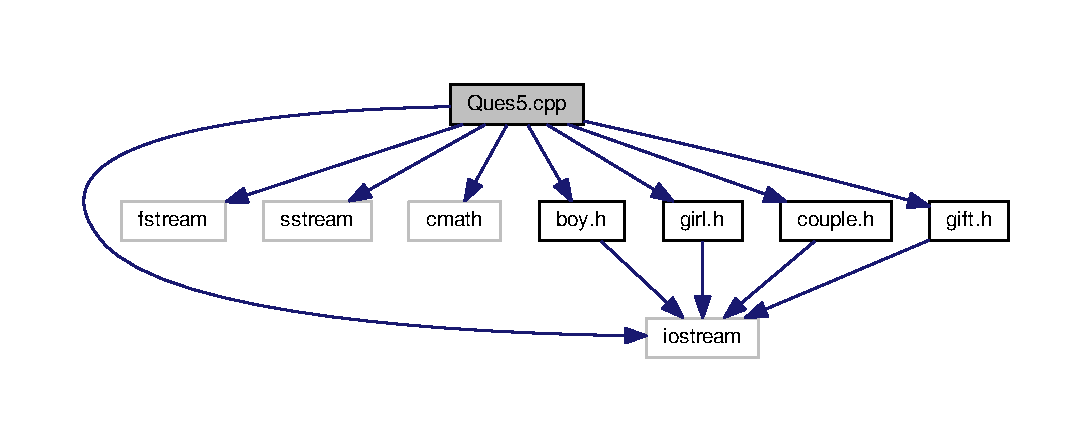
\includegraphics[width=350pt]{Ques5_8cpp__incl}
\end{center}
\end{figure}
\subsection*{Macros}
\begin{DoxyCompactItemize}
\item 
\#define \hyperlink{Ques5_8cpp_a111da81ae5883147168bbb8366377b10}{B}~9
\item 
\#define \hyperlink{Ques5_8cpp_aed9ea78689ecce0b7264c02c7f8a9a54}{G}~5
\item 
\#define \hyperlink{Ques5_8cpp_ac4cf4b2ab929bd23951a8676eeac086b}{C}~5
\item 
\#define \hyperlink{Ques5_8cpp_a5e0c07e523d4e77a2cafca06feb836f6}{Gf}~15
\item 
\#define \hyperlink{Ques5_8cpp_a97d832ae23af4f215e801e37e4f94254}{K}~3
\end{DoxyCompactItemize}
\subsection*{Functions}
\begin{DoxyCompactItemize}
\item 
void \hyperlink{Ques5_8cpp_ac70f752855ee1cf9ceaa2d749bbad17d}{swap} (\hyperlink{classGift}{Gift} \&a, \hyperlink{classGift}{Gift} \&b)
\item 
void \hyperlink{Ques5_8cpp_a9ed5e5ebda90f206f83cd424ebebe79d}{swapC} (\hyperlink{classCouple}{Couple} \&a, \hyperlink{classCouple}{Couple} \&b)
\item 
void \hyperlink{Ques5_8cpp_af29aa66b948070a74f984d5e5eae8bc0}{swapB} (\hyperlink{classBoy}{Boy} \&a, \hyperlink{classBoy}{Boy} \&b)
\item 
void \hyperlink{Ques5_8cpp_ad618e99d9871e8b49b780e086e610102}{swapG} (\hyperlink{classGirl}{Girl} \&a, \hyperlink{classGirl}{Girl} \&b)
\item 
int \hyperlink{Ques5_8cpp_ae66f6b31b5ad750f1fe042a706a4e3d4}{main} ()
\end{DoxyCompactItemize}


\subsection{Macro Definition Documentation}
\index{Ques5.\+cpp@{Ques5.\+cpp}!B@{B}}
\index{B@{B}!Ques5.\+cpp@{Ques5.\+cpp}}
\subsubsection[{\texorpdfstring{B}{B}}]{\setlength{\rightskip}{0pt plus 5cm}\#define B~9}\hypertarget{Ques5_8cpp_a111da81ae5883147168bbb8366377b10}{}\label{Ques5_8cpp_a111da81ae5883147168bbb8366377b10}
\index{Ques5.\+cpp@{Ques5.\+cpp}!C@{C}}
\index{C@{C}!Ques5.\+cpp@{Ques5.\+cpp}}
\subsubsection[{\texorpdfstring{C}{C}}]{\setlength{\rightskip}{0pt plus 5cm}\#define C~5}\hypertarget{Ques5_8cpp_ac4cf4b2ab929bd23951a8676eeac086b}{}\label{Ques5_8cpp_ac4cf4b2ab929bd23951a8676eeac086b}
\index{Ques5.\+cpp@{Ques5.\+cpp}!G@{G}}
\index{G@{G}!Ques5.\+cpp@{Ques5.\+cpp}}
\subsubsection[{\texorpdfstring{G}{G}}]{\setlength{\rightskip}{0pt plus 5cm}\#define G~5}\hypertarget{Ques5_8cpp_aed9ea78689ecce0b7264c02c7f8a9a54}{}\label{Ques5_8cpp_aed9ea78689ecce0b7264c02c7f8a9a54}
\index{Ques5.\+cpp@{Ques5.\+cpp}!Gf@{Gf}}
\index{Gf@{Gf}!Ques5.\+cpp@{Ques5.\+cpp}}
\subsubsection[{\texorpdfstring{Gf}{Gf}}]{\setlength{\rightskip}{0pt plus 5cm}\#define Gf~15}\hypertarget{Ques5_8cpp_a5e0c07e523d4e77a2cafca06feb836f6}{}\label{Ques5_8cpp_a5e0c07e523d4e77a2cafca06feb836f6}
\index{Ques5.\+cpp@{Ques5.\+cpp}!K@{K}}
\index{K@{K}!Ques5.\+cpp@{Ques5.\+cpp}}
\subsubsection[{\texorpdfstring{K}{K}}]{\setlength{\rightskip}{0pt plus 5cm}\#define K~3}\hypertarget{Ques5_8cpp_a97d832ae23af4f215e801e37e4f94254}{}\label{Ques5_8cpp_a97d832ae23af4f215e801e37e4f94254}


\subsection{Function Documentation}
\index{Ques5.\+cpp@{Ques5.\+cpp}!main@{main}}
\index{main@{main}!Ques5.\+cpp@{Ques5.\+cpp}}
\subsubsection[{\texorpdfstring{main()}{main()}}]{\setlength{\rightskip}{0pt plus 5cm}int main (
\begin{DoxyParamCaption}
{}
\end{DoxyParamCaption}
)}\hypertarget{Ques5_8cpp_ae66f6b31b5ad750f1fe042a706a4e3d4}{}\label{Ques5_8cpp_ae66f6b31b5ad750f1fe042a706a4e3d4}

\begin{DoxyCode}
49 \{
50     \hyperlink{classBoy}{Boy} boys[\hyperlink{Ques5_8cpp_a111da81ae5883147168bbb8366377b10}{B}];
51     \hyperlink{classGirl}{Girl} girls[\hyperlink{Ques5_8cpp_aed9ea78689ecce0b7264c02c7f8a9a54}{G}];
52     \hyperlink{classCouple}{Couple} couples[\hyperlink{Ques5_8cpp_ac4cf4b2ab929bd23951a8676eeac086b}{C}];
53     \hyperlink{classGift}{Gift} gifts[\hyperlink{Ques5_8cpp_a5e0c07e523d4e77a2cafca06feb836f6}{Gf}];
54     
55     \textcolor{keywordtype}{string} line;
56     \textcolor{keywordtype}{int} c = 0, x = 0;
57 
58     ofstream logFile;
59     logFile.open(\textcolor{stringliteral}{"logFile5.dat"});
60 
61 
62     
63     \textcolor{comment}{/*}
64 \textcolor{comment}{     *taking input from boy.dat}
65 \textcolor{comment}{     */}
66     ifstream boyInp(\textcolor{stringliteral}{"boy.dat"});
67     \textcolor{keywordflow}{while}(getline(boyInp,line)) \{
68         \textcolor{keywordflow}{if}(c++ == 0) \textcolor{keywordflow}{continue};
69         istringstream iss(line);
70         \textcolor{keywordtype}{string} name;
71         \textcolor{keywordtype}{int} a,i,b,t,s;
72         \textcolor{keywordtype}{char} ty;
73         \textcolor{keywordflow}{if}((iss>>name>>a>>i>>b>>t>>s>>ty))\{
74             boys[x++].\hyperlink{classBoy_a6ac70867d517f6b429ce67c8eb2915ed}{setDetails}(name,a,i,b,t,s,ty);
75         \} \textcolor{keywordflow}{else} \{
76             \textcolor{keywordflow}{break};
77         \}
78     \}
79 
80     c = 0;
81     x = 0;
82     \textcolor{comment}{/*}
83 \textcolor{comment}{     *taking input from girl.dat}
84 \textcolor{comment}{     */}
85     ifstream girlInp(\textcolor{stringliteral}{"girl.dat"});
86     \textcolor{keywordflow}{while}(getline(girlInp,line)) \{
87         \textcolor{keywordflow}{if}(c++ == 0) \textcolor{keywordflow}{continue};
88         istringstream iss(line);
89         \textcolor{keywordtype}{string} name;
90         \textcolor{keywordtype}{int} a,i,m,s;
91         \textcolor{keywordtype}{char} ty,cr;
92         \textcolor{keywordflow}{if}((iss>>name>>a>>i>>m>>cr>>s>>ty))\{
93             girls[x++].\hyperlink{classGirl_a4bff314dba17278eb1093b15f7be80bd}{setDetails}(name,a,i,m,ty,s,cr);
94         \} \textcolor{keywordflow}{else} \{
95             \textcolor{keywordflow}{break};
96         \}
97     \}
98 
99     c = 0;
100     x = 0;
101     \textcolor{comment}{/*}
102 \textcolor{comment}{     *taking input from gift.dat}
103 \textcolor{comment}{     */} 
104     ifstream giftInp(\textcolor{stringliteral}{"gift.dat"});
105     \textcolor{keywordflow}{while}(getline(giftInp,line)) \{
106         \textcolor{keywordflow}{if}(c++ == 0) \textcolor{keywordflow}{continue};
107         istringstream iss(line);
108         \textcolor{keywordtype}{int} id,p,v;
109         \textcolor{keywordtype}{char} ty;
110         \textcolor{keywordflow}{if}((iss>>\textcolor{keywordtype}{id}>>p>>ty>>v))\{
111             gifts[x++].\hyperlink{classGift_abc74fbed8b31b5bb7745b3e0c934da9e}{setDetail}(\textcolor{keywordtype}{id},p,ty,0);
112         \} \textcolor{keywordflow}{else} \{
113             \textcolor{keywordflow}{break};
114         \}
115     \}
116 
117     \textcolor{comment}{/*}
118 \textcolor{comment}{     * sorting boys}
119 \textcolor{comment}{     */}
120     \textcolor{keywordflow}{for}(\textcolor{keywordtype}{int} i = 0  ; i< \hyperlink{Ques5_8cpp_a111da81ae5883147168bbb8366377b10}{B}-1; i++) \{
121         \textcolor{keywordflow}{for}(\textcolor{keywordtype}{int} j = i+1; j < \hyperlink{Ques5_8cpp_a111da81ae5883147168bbb8366377b10}{B}; j++) \{
122             \textcolor{keywordflow}{if}(boys[i].getAttractiveness() > boys[j].getAttractiveness()) \{
123                 \hyperlink{Ques5_8cpp_af29aa66b948070a74f984d5e5eae8bc0}{swapB}(boys[i],boys[j]);
124             \}   
125         \}
126     \}
127 
128     \textcolor{comment}{/*}
129 \textcolor{comment}{     *sorting girls}
130 \textcolor{comment}{     */}
131     \textcolor{keywordflow}{for}(\textcolor{keywordtype}{int} i = 0  ; i< \hyperlink{Ques5_8cpp_aed9ea78689ecce0b7264c02c7f8a9a54}{G}-1; i++) \{
132         \textcolor{keywordflow}{for}(\textcolor{keywordtype}{int} j = i+1; j < \hyperlink{Ques5_8cpp_aed9ea78689ecce0b7264c02c7f8a9a54}{G}; j++) \{
133             \textcolor{keywordflow}{if}(girls[i].getMaintenance() > girls[j].getMaintenance()) \{
134                 \hyperlink{Ques5_8cpp_ad618e99d9871e8b49b780e086e610102}{swapG}(girls[i],girls[j]);
135             \}   
136         \}
137     \}
138     
139     c = 0;
140     \textcolor{keywordtype}{int} i = 0;
141     \textcolor{comment}{/*}
142 \textcolor{comment}{     *Forming Couples}
143 \textcolor{comment}{     */}
144     \textcolor{keywordflow}{for}(\textcolor{keywordtype}{int} m = 0 ; m < \hyperlink{Ques5_8cpp_aed9ea78689ecce0b7264c02c7f8a9a54}{G}; m++) \{
145         \textcolor{keywordflow}{if}(m %2 == 0) \{     \textcolor{comment}{//assigning a boy to a girl}
146             \textcolor{keywordflow}{while}(girls[i].getStatus() != 0 && i != G)i++;
147  
148             \textcolor{keywordflow}{if}(i == G) \textcolor{keywordflow}{break};
149 
150             \textcolor{keywordflow}{if}(girls[i].getCriterion() == \textcolor{charliteral}{'A'}) \{
151                 \textcolor{keywordtype}{int} max= -99;
152                 \textcolor{keywordtype}{int} ind = -1;
153                 \textcolor{keywordflow}{for}(\textcolor{keywordtype}{int} j = 0; j < \hyperlink{Ques5_8cpp_a111da81ae5883147168bbb8366377b10}{B}; j++) \{
154                     \textcolor{keywordflow}{if}(boys[j].getAttractiveness() > max && boys[j].getStatus() == 0) \{
155                         \textcolor{keywordflow}{if}(boys[j].getBudget() > girls[i].getMaintenance()) \{
156                             \textcolor{keywordflow}{if}(girls[i].getAttractiveness() > boys[j].getThreshold()) \{
157                                 max = boys[j].\hyperlink{classBoy_a814ef4919f2ac86c6ee70f9698afad3d}{getAttractiveness}();
158                                 ind = j;
159                             \}
160                         \}
161                     \}
162                 \}
163         
164                 \textcolor{keywordflow}{if}(ind != -1) \{
165                     boys[ind].\hyperlink{classBoy_a3d29dcc4137fbfc0306cbd7df82781c3}{setStatus}(1);
166                     girls[i].\hyperlink{classGirl_a201527323b3fabac4b089f003b8fcc4a}{setStatus}(1);
167                     couples[c++].\hyperlink{classCouple_a0057d3dfd3939a156cd99f6c5cf32279}{setDetails}(boys[ind].getName(),girls[i].getname()) ; 
168                 \}       
169             \} \textcolor{keywordflow}{else} \textcolor{keywordflow}{if}(girls[i].getCriterion() == \textcolor{charliteral}{'I'}) \{
170                 \textcolor{keywordtype}{int} max= -99;
171                         \textcolor{keywordtype}{int} ind = -1;
172                         \textcolor{keywordflow}{for}(\textcolor{keywordtype}{int} j = 0; j < \hyperlink{Ques5_8cpp_a111da81ae5883147168bbb8366377b10}{B}; j++) \{
173                                 \textcolor{keywordflow}{if}(boys[j].getIntelligence() > max && boys[j].getStatus() == 0) \{
174                                         \textcolor{keywordflow}{if}(boys[j].getBudget() > girls[i].getMaintenance()) \{
175                                                 \textcolor{keywordflow}{if}(girls[i].getAttractiveness() > boys[j].getThreshold()) \{
176                                                         max = boys[j].
      \hyperlink{classBoy_ad52c9e04ab591f3909d2342d6cae0168}{getIntelligence}();
177                                                         ind = j;
178                                                 \}
179                                         \}
180                                 \}
181                         \}
182                           
183                         \textcolor{keywordflow}{if}(ind != -1) \{
184                                 boys[ind].\hyperlink{classBoy_a3d29dcc4137fbfc0306cbd7df82781c3}{setStatus}(1);
185                                 girls[i].\hyperlink{classGirl_a201527323b3fabac4b089f003b8fcc4a}{setStatus}(1);
186                                 couples[c++].\hyperlink{classCouple_a0057d3dfd3939a156cd99f6c5cf32279}{setDetails}(boys[ind].getName(),girls[i].getname()) ;
187                         \}
188 
189             \} \textcolor{keywordflow}{else} \{
190                 \textcolor{keywordtype}{int} max= -99;
191                         \textcolor{keywordtype}{int} ind = -1;
192                         \textcolor{keywordflow}{for}(\textcolor{keywordtype}{int} j = 0; j < \hyperlink{Ques5_8cpp_a111da81ae5883147168bbb8366377b10}{B}; j++) \{
193                                 \textcolor{keywordflow}{if}(boys[j].getBudget() > max && boys[j].getStatus() == 0) \{
194                                         \textcolor{keywordflow}{if}(boys[j].getBudget() > girls[i].getMaintenance()) \{
195                                                 \textcolor{keywordflow}{if}(girls[i].getAttractiveness() > boys[j].getThreshold()) \{
196                                                         max = boys[j].\hyperlink{classBoy_a05c48b12091ebcad44ba86ba88514ac5}{getBudget}();
197                                                         ind = j;
198                                                 \}
199                                         \}
200                                 \}
201                         \}
202                           
203                         \textcolor{keywordflow}{if}(ind != -1) \{
204                                 boys[ind].\hyperlink{classBoy_a3d29dcc4137fbfc0306cbd7df82781c3}{setStatus}(1);
205                                 girls[i].\hyperlink{classGirl_a201527323b3fabac4b089f003b8fcc4a}{setStatus}(1);
206                                 couples[c++].\hyperlink{classCouple_a0057d3dfd3939a156cd99f6c5cf32279}{setDetails}(boys[ind].getName(),girls[i].getname()) ;
207                         \}
208             
209             \}
210         \} \textcolor{keywordflow}{else} \{        \textcolor{comment}{//assigning a girl to a boy}
211             \textcolor{keywordflow}{for}(\textcolor{keywordtype}{int} j = 0; j < \hyperlink{Ques5_8cpp_a111da81ae5883147168bbb8366377b10}{B}; j++) \{
212                 \textcolor{keywordflow}{if}(boys[j].getStatus() == 0) \{
213                     \textcolor{keywordtype}{int} ind = -1;
214                     \textcolor{keywordtype}{int} max = -99;
215                     \textcolor{keywordflow}{for}(\textcolor{keywordtype}{int} k = 0; k < \hyperlink{Ques5_8cpp_aed9ea78689ecce0b7264c02c7f8a9a54}{G}; k++) \{
216                         \textcolor{keywordflow}{if}(girls[k].getStatus() == 0 && girls[i].getAttractiveness() > max) \{
217                             max = girls[i].\hyperlink{classGirl_a04cfe3e0c21240f92c19152630a40252}{getAttractiveness}();
218                             ind = k;
219                         \} 
220                         
221                     \}
222                     boys[j].\hyperlink{classBoy_a3d29dcc4137fbfc0306cbd7df82781c3}{setStatus}(1);
223                                 girls[ind].\hyperlink{classGirl_a201527323b3fabac4b089f003b8fcc4a}{setStatus}(1);
224                     couples[c++].\hyperlink{classCouple_a0057d3dfd3939a156cd99f6c5cf32279}{setDetails}(boys[j].getName(),girls[ind].getname()) ;
225                     \textcolor{keywordflow}{break};
226                 \}
227             \}
228         \}
229     \}
230 
231     \textcolor{comment}{/*}
232 \textcolor{comment}{     *Printing couples}
233 \textcolor{comment}{     */}
234     logFile<<\textcolor{stringliteral}{"-----------------COUPLES-------------------\(\backslash\)n\(\backslash\)n"};
235 
236     \textcolor{keywordflow}{for}(\textcolor{keywordtype}{int} i = 0 ;i < \hyperlink{Ques5_8cpp_ac4cf4b2ab929bd23951a8676eeac086b}{C}; i++) \{
237         logFile<<\textcolor{stringliteral}{"Boy b"}<<couples[i].\hyperlink{classCouple_a092cbc580ea255febc3eb211c5f56512}{getBoy}()<<\textcolor{stringliteral}{" and Girl g"}<<couples[i].
      \hyperlink{classCouple_a653983df7e331c0534ae2ce42e9856c5}{getGirl}()<<\textcolor{stringliteral}{"\(\backslash\)n"};
238         
239     \}
240 
241     \textcolor{comment}{/*}
242 \textcolor{comment}{     *Sorting gifts}
243 \textcolor{comment}{     */}
244     \textcolor{keywordflow}{for}(\textcolor{keywordtype}{int} i = 0  ; i< \hyperlink{Ques5_8cpp_a5e0c07e523d4e77a2cafca06feb836f6}{Gf}-1; i++) \{
245         \textcolor{keywordflow}{for}(\textcolor{keywordtype}{int} j = i+1; j < \hyperlink{Ques5_8cpp_a5e0c07e523d4e77a2cafca06feb836f6}{Gf}; j++) \{
246             \textcolor{keywordflow}{if}(gifts[j].getprice() < gifts[i].getprice()) \{
247                 \hyperlink{Ques5_8cpp_ac70f752855ee1cf9ceaa2d749bbad17d}{swap}(gifts[j],gifts[i]);
248             \}
249         \}
250     \}
251 
252     \textcolor{comment}{/*}
253 \textcolor{comment}{     *Assigning gifts to couples}
254 \textcolor{comment}{     */}
255     \textcolor{keywordflow}{for}(\textcolor{keywordtype}{int} i  = 0 ;i < \hyperlink{Ques5_8cpp_ac4cf4b2ab929bd23951a8676eeac086b}{C}; i++) \{
256         \textcolor{keywordtype}{int} boy = couples[i].\hyperlink{classCouple_a092cbc580ea255febc3eb211c5f56512}{getBoy}()[0] - 48;
257         \textcolor{keywordtype}{int} girl = couples[i].\hyperlink{classCouple_a653983df7e331c0534ae2ce42e9856c5}{getGirl}()[0] - 48;
258         \textcolor{keywordtype}{int} mc = girls[girl-1].\hyperlink{classGirl_a6192affb0721b385d2c5d83a011a869e}{getMaintenance}();
259         \textcolor{keywordtype}{int} bud = boys[boy-1].\hyperlink{classBoy_a05c48b12091ebcad44ba86ba88514ac5}{getBudget}();
260         \textcolor{keywordtype}{int} x = bud - mc;
261         \textcolor{keywordtype}{char} bt = boys[boy-1].\hyperlink{classBoy_a01accc077c0824f7e28cfe391f7851c7}{getType}(); 
262     
263         \textcolor{keywordflow}{if}(bt == \textcolor{charliteral}{'M'}) \{
264             \textcolor{keywordflow}{for}(\textcolor{keywordtype}{int} j = 0 ; j < \hyperlink{Ques5_8cpp_a5e0c07e523d4e77a2cafca06feb836f6}{Gf}; j++) \{
265                 
266                 \textcolor{keywordflow}{if}(gifts[j].getprice() <= mc && gifts[j].getStatus() == 0) \{
267                     couples[i].\hyperlink{classCouple_a1a621700c479fd808b0caf034f4bd0f5}{setGifts}(j+1);
268                     gifts[j].\hyperlink{classGift_a8c8a8be33c3abe17bbe4b8da9ac084d6}{setStatus}(1);
269                     mc = mc - gifts[j].\hyperlink{classGift_aa36f2b437e93ede1d2569e489b493441}{getprice}();
270                 \} \textcolor{keywordflow}{else} \textcolor{keywordflow}{if}( gifts[j].getprice() <= x +mc ) \{
271                     \textcolor{keywordflow}{if}( gifts[j].getStatus() == 0)  \{               
272                         couples[i].\hyperlink{classCouple_a1a621700c479fd808b0caf034f4bd0f5}{setGifts}(j+1);
273                         gifts[j].\hyperlink{classGift_a8c8a8be33c3abe17bbe4b8da9ac084d6}{setStatus}(1);
274                         \textcolor{keywordflow}{break};
275                     \}
276                 \} \textcolor{keywordflow}{else} \{
277                     \textcolor{keywordflow}{break};
278                 \}
279             \} 
280         \} \textcolor{keywordflow}{else}  \textcolor{keywordflow}{if}(bt == \textcolor{charliteral}{'N'}) \{
281             \textcolor{keywordflow}{for}(\textcolor{keywordtype}{int} j = Gf-1 ; j >= 0; j--) \{
282                 \textcolor{keywordflow}{if}(gifts[j].getprice() <= bud && gifts[j].getStatus() == 0) \{
283                     couples[i].\hyperlink{classCouple_a1a621700c479fd808b0caf034f4bd0f5}{setGifts}(j+1);
284                     gifts[j].\hyperlink{classGift_a8c8a8be33c3abe17bbe4b8da9ac084d6}{setStatus}(1);
285                     bud = bud- gifts[j].\hyperlink{classGift_aa36f2b437e93ede1d2569e489b493441}{getprice}();
286                 \}
287             \}
288         \} \textcolor{keywordflow}{else} \{
289             \textcolor{keywordflow}{for}(\textcolor{keywordtype}{int} j = 0 ; j < \hyperlink{Ques5_8cpp_a5e0c07e523d4e77a2cafca06feb836f6}{Gf}; j++) \{
290                 \textcolor{keywordflow}{if}(gifts[j].getprice() <= mc && gifts[j].getStatus() == 0) \{
291                     couples[i].\hyperlink{classCouple_a1a621700c479fd808b0caf034f4bd0f5}{setGifts}(j+1);
292                     gifts[j].\hyperlink{classGift_a8c8a8be33c3abe17bbe4b8da9ac084d6}{setStatus}(1);
293                     mc = mc - gifts[j].\hyperlink{classGift_aa36f2b437e93ede1d2569e489b493441}{getprice}();
294                 \}\textcolor{keywordflow}{else} \textcolor{keywordflow}{if}(gifts[j].getprice() <= x +mc) \{
295                     \textcolor{keywordflow}{if}( gifts[j].getStatus() == 0)  \{               
296                         couples[i].\hyperlink{classCouple_a1a621700c479fd808b0caf034f4bd0f5}{setGifts}(j+1);
297                         gifts[j].\hyperlink{classGift_a8c8a8be33c3abe17bbe4b8da9ac084d6}{setStatus}(1);
298                         \textcolor{keywordflow}{break};
299                     \}
300                 \} \textcolor{keywordflow}{else} \{
301                     \textcolor{keywordflow}{break};
302                 \}
303             \}
304         \}
305     \}
306     
307     
308 
309     \textcolor{comment}{/*}
310 \textcolor{comment}{     *Calculating Happiness}
311 \textcolor{comment}{     */}
312     \textcolor{keywordflow}{for}(\textcolor{keywordtype}{int} i = 0; i < \hyperlink{Ques5_8cpp_ac4cf4b2ab929bd23951a8676eeac086b}{C}; i++) \{
313         \textcolor{keywordtype}{int} boy = couples[i].\hyperlink{classCouple_a092cbc580ea255febc3eb211c5f56512}{getBoy}()[0] - 48;
314         \textcolor{keywordtype}{int} girl = couples[i].\hyperlink{classCouple_a653983df7e331c0534ae2ce42e9856c5}{getGirl}()[0] - 48;
315 
316         \textcolor{keywordtype}{int} mc = girls[girl-1].\hyperlink{classGirl_a6192affb0721b385d2c5d83a011a869e}{getMaintenance}();
317         \textcolor{keywordtype}{int} bud = boys[boy-1].\hyperlink{classBoy_a05c48b12091ebcad44ba86ba88514ac5}{getBudget}();
318         \textcolor{keywordtype}{int} x1 = bud - mc;
319 
320         \textcolor{keywordtype}{char} bt = boys[boy-1].\hyperlink{classBoy_a01accc077c0824f7e28cfe391f7851c7}{getType}();
321         \textcolor{keywordtype}{char} gt = girls[girl-1].\hyperlink{classGirl_af26252dbf5784c2c79744dd4652a3bf2}{getType}();
322         
323         \textcolor{keywordtype}{int} hb = 0;
324         \textcolor{keywordtype}{int} hg = 0;
325 
326         \textcolor{keywordtype}{int} total = 0;
327     
328         
329         \textcolor{keywordtype}{int} * arr = couples[i].\hyperlink{classCouple_a80cef2647acb3903936372a0d70cf9cc}{getGifts}();
330         \textcolor{keywordflow}{for}(\textcolor{keywordtype}{int} j = 0 ; j < couples[i].\hyperlink{classCouple_a05a3bbd0d8d6b149ae04f5306acd4439}{getNum}(); j++) \{
331             total += gifts[arr[j]-1].\hyperlink{classGift_aa36f2b437e93ede1d2569e489b493441}{getprice}();
332         \}
333     
334         \textcolor{keywordflow}{if}(bt == \textcolor{charliteral}{'M'}) \{
335             hb = bud-total;
336         \} \textcolor{keywordflow}{else} \textcolor{keywordflow}{if}(bt == \textcolor{charliteral}{'N'}) \{
337             hb = hg;
338         \} \textcolor{keywordflow}{else} \{
339             hb = girls[girl-1].\hyperlink{classGirl_afe73c4c4f180aa8f5e0bc4f87455ec0b}{getIntelligence}();
340         \}
341 
342         \textcolor{keywordflow}{if}(gt == \textcolor{charliteral}{'C'}) \{
343             hg = log(abs(mc-total));
344         \} \textcolor{keywordflow}{else} \textcolor{keywordflow}{if}(gt == \textcolor{charliteral}{'N'}) \{
345             hg = abs(mc-total);
346         \} \textcolor{keywordflow}{else} \{
347             hg = exp(abs(mc-total));
348         \}
349         couples[i].\hyperlink{classCouple_a19afd8575f26caa557115a106b6a4928}{setHappiness}(hb + abs(hg));
350         
351     \}
352 
353 
354     \textcolor{comment}{/*}
355 \textcolor{comment}{     *sorting couples according to happiness}
356 \textcolor{comment}{     */}
357     \textcolor{keywordflow}{for}(\textcolor{keywordtype}{int} i = 0  ; i< C-1; i++) \{
358         \textcolor{keywordflow}{for}(\textcolor{keywordtype}{int} j = i+1; j < \hyperlink{Ques5_8cpp_ac4cf4b2ab929bd23951a8676eeac086b}{C}; j++) \{
359             \textcolor{keywordflow}{if}(couples[i].getHappiness() > couples[j].getHappiness()) \{
360                 \hyperlink{Ques5_8cpp_a9ed5e5ebda90f206f83cd424ebebe79d}{swapC}(couples[i],couples[j]);
361             \}   
362         \}
363     \}
364     
365     \textcolor{comment}{/*}
366 \textcolor{comment}{     *Printing k most happy couples}
367 \textcolor{comment}{     */}
368     logFile<<\textcolor{stringliteral}{"\(\backslash\)n---------------------K(== 3) Most Happy Couples------------------------\(\backslash\)n\(\backslash\)n"};
369     \textcolor{keywordflow}{for}(\textcolor{keywordtype}{int} i = C-1; i >C-\hyperlink{Ques5_8cpp_a97d832ae23af4f215e801e37e4f94254}{K}-1 ;i--) \{
370         logFile<<\textcolor{stringliteral}{"Boy b"}<<couples[i].\hyperlink{classCouple_a092cbc580ea255febc3eb211c5f56512}{getBoy}()<<\textcolor{stringliteral}{" and Girl g"}<<couples[i].
      \hyperlink{classCouple_a653983df7e331c0534ae2ce42e9856c5}{getGirl}()<<\textcolor{stringliteral}{"\(\backslash\)n"};
371     \}
372 
373 
374 
375     logFile.close();
376 \}
\end{DoxyCode}
\index{Ques5.\+cpp@{Ques5.\+cpp}!swap@{swap}}
\index{swap@{swap}!Ques5.\+cpp@{Ques5.\+cpp}}
\subsubsection[{\texorpdfstring{swap(\+Gift \&a, Gift \&b)}{swap(Gift &a, Gift &b)}}]{\setlength{\rightskip}{0pt plus 5cm}void swap (
\begin{DoxyParamCaption}
\item[{{\bf Gift} \&}]{a, }
\item[{{\bf Gift} \&}]{b}
\end{DoxyParamCaption}
)}\hypertarget{Ques5_8cpp_ac70f752855ee1cf9ceaa2d749bbad17d}{}\label{Ques5_8cpp_ac70f752855ee1cf9ceaa2d749bbad17d}

\begin{DoxyCode}
21 \{
22     \hyperlink{classGift}{Gift} temp = a;
23     a = b;
24     b = temp;
25 \}
\end{DoxyCode}
\index{Ques5.\+cpp@{Ques5.\+cpp}!swapB@{swapB}}
\index{swapB@{swapB}!Ques5.\+cpp@{Ques5.\+cpp}}
\subsubsection[{\texorpdfstring{swap\+B(\+Boy \&a, Boy \&b)}{swapB(Boy &a, Boy &b)}}]{\setlength{\rightskip}{0pt plus 5cm}void swapB (
\begin{DoxyParamCaption}
\item[{{\bf Boy} \&}]{a, }
\item[{{\bf Boy} \&}]{b}
\end{DoxyParamCaption}
)}\hypertarget{Ques5_8cpp_af29aa66b948070a74f984d5e5eae8bc0}{}\label{Ques5_8cpp_af29aa66b948070a74f984d5e5eae8bc0}

\begin{DoxyCode}
35 \{
36     \hyperlink{classBoy}{Boy} temp = a;
37     a = b;
38     b = temp;
39 \}
\end{DoxyCode}
\index{Ques5.\+cpp@{Ques5.\+cpp}!swapC@{swapC}}
\index{swapC@{swapC}!Ques5.\+cpp@{Ques5.\+cpp}}
\subsubsection[{\texorpdfstring{swap\+C(\+Couple \&a, Couple \&b)}{swapC(Couple &a, Couple &b)}}]{\setlength{\rightskip}{0pt plus 5cm}void swapC (
\begin{DoxyParamCaption}
\item[{{\bf Couple} \&}]{a, }
\item[{{\bf Couple} \&}]{b}
\end{DoxyParamCaption}
)}\hypertarget{Ques5_8cpp_a9ed5e5ebda90f206f83cd424ebebe79d}{}\label{Ques5_8cpp_a9ed5e5ebda90f206f83cd424ebebe79d}

\begin{DoxyCode}
28 \{
29     \hyperlink{classCouple}{Couple} temp = a;
30     a = b;
31     b = temp;
32 \}
\end{DoxyCode}
\index{Ques5.\+cpp@{Ques5.\+cpp}!swapG@{swapG}}
\index{swapG@{swapG}!Ques5.\+cpp@{Ques5.\+cpp}}
\subsubsection[{\texorpdfstring{swap\+G(\+Girl \&a, Girl \&b)}{swapG(Girl &a, Girl &b)}}]{\setlength{\rightskip}{0pt plus 5cm}void swapG (
\begin{DoxyParamCaption}
\item[{{\bf Girl} \&}]{a, }
\item[{{\bf Girl} \&}]{b}
\end{DoxyParamCaption}
)}\hypertarget{Ques5_8cpp_ad618e99d9871e8b49b780e086e610102}{}\label{Ques5_8cpp_ad618e99d9871e8b49b780e086e610102}

\begin{DoxyCode}
42 \{
43     \hyperlink{classGirl}{Girl} temp = a;
44     a = b;
45     b = temp;
46 \}
\end{DoxyCode}

\hypertarget{Ques6_8cpp}{}\section{Ques6.\+cpp File Reference}
\label{Ques6_8cpp}\index{Ques6.\+cpp@{Ques6.\+cpp}}
{\ttfamily \#include $<$iostream$>$}\\*
{\ttfamily \#include $<$fstream$>$}\\*
{\ttfamily \#include $<$sstream$>$}\\*
{\ttfamily \#include $<$cmath$>$}\\*
{\ttfamily \#include \char`\"{}boy.\+h\char`\"{}}\\*
{\ttfamily \#include \char`\"{}girl.\+h\char`\"{}}\\*
{\ttfamily \#include \char`\"{}couple.\+h\char`\"{}}\\*
{\ttfamily \#include \char`\"{}gift.\+h\char`\"{}}\\*
Include dependency graph for Ques6.\+cpp\+:
\nopagebreak
\begin{figure}[H]
\begin{center}
\leavevmode
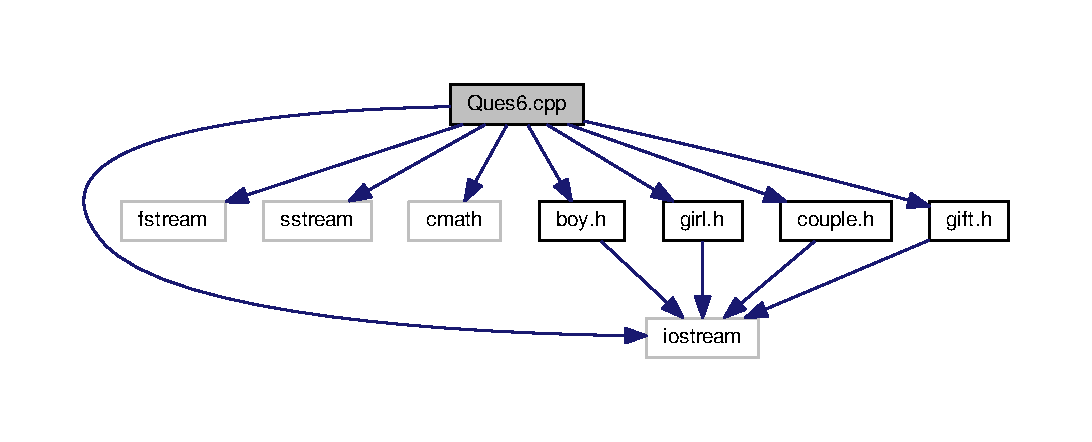
\includegraphics[width=350pt]{Ques6_8cpp__incl}
\end{center}
\end{figure}
\subsection*{Macros}
\begin{DoxyCompactItemize}
\item 
\#define \hyperlink{Ques6_8cpp_a111da81ae5883147168bbb8366377b10}{B}~9
\item 
\#define \hyperlink{Ques6_8cpp_aed9ea78689ecce0b7264c02c7f8a9a54}{G}~5
\item 
\#define \hyperlink{Ques6_8cpp_ac4cf4b2ab929bd23951a8676eeac086b}{C}~5
\item 
\#define \hyperlink{Ques6_8cpp_a5e0c07e523d4e77a2cafca06feb836f6}{Gf}~15
\item 
\#define \hyperlink{Ques6_8cpp_a0acb682b8260ab1c60b918599864e2e5}{T}~5
\end{DoxyCompactItemize}
\subsection*{Functions}
\begin{DoxyCompactItemize}
\item 
void \hyperlink{Ques6_8cpp_ac70f752855ee1cf9ceaa2d749bbad17d}{swap} (\hyperlink{classGift}{Gift} \&a, \hyperlink{classGift}{Gift} \&b)
\item 
void \hyperlink{Ques6_8cpp_a9ed5e5ebda90f206f83cd424ebebe79d}{swapC} (\hyperlink{classCouple}{Couple} \&a, \hyperlink{classCouple}{Couple} \&b)
\item 
int \hyperlink{Ques6_8cpp_ae66f6b31b5ad750f1fe042a706a4e3d4}{main} ()
\end{DoxyCompactItemize}


\subsection{Macro Definition Documentation}
\index{Ques6.\+cpp@{Ques6.\+cpp}!B@{B}}
\index{B@{B}!Ques6.\+cpp@{Ques6.\+cpp}}
\subsubsection[{\texorpdfstring{B}{B}}]{\setlength{\rightskip}{0pt plus 5cm}\#define B~9}\hypertarget{Ques6_8cpp_a111da81ae5883147168bbb8366377b10}{}\label{Ques6_8cpp_a111da81ae5883147168bbb8366377b10}
\index{Ques6.\+cpp@{Ques6.\+cpp}!C@{C}}
\index{C@{C}!Ques6.\+cpp@{Ques6.\+cpp}}
\subsubsection[{\texorpdfstring{C}{C}}]{\setlength{\rightskip}{0pt plus 5cm}\#define C~5}\hypertarget{Ques6_8cpp_ac4cf4b2ab929bd23951a8676eeac086b}{}\label{Ques6_8cpp_ac4cf4b2ab929bd23951a8676eeac086b}
\index{Ques6.\+cpp@{Ques6.\+cpp}!G@{G}}
\index{G@{G}!Ques6.\+cpp@{Ques6.\+cpp}}
\subsubsection[{\texorpdfstring{G}{G}}]{\setlength{\rightskip}{0pt plus 5cm}\#define G~5}\hypertarget{Ques6_8cpp_aed9ea78689ecce0b7264c02c7f8a9a54}{}\label{Ques6_8cpp_aed9ea78689ecce0b7264c02c7f8a9a54}
\index{Ques6.\+cpp@{Ques6.\+cpp}!Gf@{Gf}}
\index{Gf@{Gf}!Ques6.\+cpp@{Ques6.\+cpp}}
\subsubsection[{\texorpdfstring{Gf}{Gf}}]{\setlength{\rightskip}{0pt plus 5cm}\#define Gf~15}\hypertarget{Ques6_8cpp_a5e0c07e523d4e77a2cafca06feb836f6}{}\label{Ques6_8cpp_a5e0c07e523d4e77a2cafca06feb836f6}
\index{Ques6.\+cpp@{Ques6.\+cpp}!T@{T}}
\index{T@{T}!Ques6.\+cpp@{Ques6.\+cpp}}
\subsubsection[{\texorpdfstring{T}{T}}]{\setlength{\rightskip}{0pt plus 5cm}\#define T~5}\hypertarget{Ques6_8cpp_a0acb682b8260ab1c60b918599864e2e5}{}\label{Ques6_8cpp_a0acb682b8260ab1c60b918599864e2e5}


\subsection{Function Documentation}
\index{Ques6.\+cpp@{Ques6.\+cpp}!main@{main}}
\index{main@{main}!Ques6.\+cpp@{Ques6.\+cpp}}
\subsubsection[{\texorpdfstring{main()}{main()}}]{\setlength{\rightskip}{0pt plus 5cm}int main (
\begin{DoxyParamCaption}
{}
\end{DoxyParamCaption}
)}\hypertarget{Ques6_8cpp_ae66f6b31b5ad750f1fe042a706a4e3d4}{}\label{Ques6_8cpp_ae66f6b31b5ad750f1fe042a706a4e3d4}

\begin{DoxyCode}
36 \{
37     \hyperlink{classBoy}{Boy} boys[\hyperlink{Ques6_8cpp_a111da81ae5883147168bbb8366377b10}{B}];
38     \hyperlink{classGirl}{Girl} girls[\hyperlink{Ques6_8cpp_aed9ea78689ecce0b7264c02c7f8a9a54}{G}];
39     \hyperlink{classCouple}{Couple} couples[\hyperlink{Ques6_8cpp_ac4cf4b2ab929bd23951a8676eeac086b}{C}];
40     \hyperlink{classGift}{Gift} gifts[\hyperlink{Ques6_8cpp_a5e0c07e523d4e77a2cafca06feb836f6}{Gf}];
41     
42     \textcolor{keywordtype}{string} line;
43     \textcolor{keywordtype}{int} c = 0, x = 0;
44 
45     ofstream logFile;
46     logFile.open(\textcolor{stringliteral}{"logFile6.dat"});
47 
48 
49     \textcolor{comment}{/*}
50 \textcolor{comment}{     *taking input from boy.dat}
51 \textcolor{comment}{     */}
52     ifstream boyInp(\textcolor{stringliteral}{"boy.dat"});
53     \textcolor{keywordflow}{while}(getline(boyInp,line)) \{
54         \textcolor{keywordflow}{if}(c++ == 0) \textcolor{keywordflow}{continue};
55         istringstream iss(line);
56         \textcolor{keywordtype}{string} name;
57         \textcolor{keywordtype}{int} a,i,b,t,s;
58         \textcolor{keywordtype}{char} ty;
59         \textcolor{keywordflow}{if}((iss>>name>>a>>i>>b>>t>>s>>ty))\{
60             boys[x++].\hyperlink{classBoy_a6ac70867d517f6b429ce67c8eb2915ed}{setDetails}(name,a,i,b,t,s,ty);
61         \} \textcolor{keywordflow}{else} \{
62             \textcolor{keywordflow}{break};
63         \}
64     \}
65 
66     c = 0;
67     x = 0;
68     \textcolor{comment}{/*}
69 \textcolor{comment}{     *taking input from girl.dat}
70 \textcolor{comment}{     */}
71     ifstream girlInp(\textcolor{stringliteral}{"girl.dat"});
72     \textcolor{keywordflow}{while}(getline(girlInp,line)) \{
73         \textcolor{keywordflow}{if}(c++ == 0) \textcolor{keywordflow}{continue};
74         istringstream iss(line);
75         \textcolor{keywordtype}{string} name;
76         \textcolor{keywordtype}{int} a,i,m,s;
77         \textcolor{keywordtype}{char} ty,cr;
78         \textcolor{keywordflow}{if}((iss>>name>>a>>i>>m>>cr>>s>>ty))\{
79             girls[x++].\hyperlink{classGirl_a4bff314dba17278eb1093b15f7be80bd}{setDetails}(name,a,i,m,ty,s,cr);
80         \} \textcolor{keywordflow}{else} \{
81             \textcolor{keywordflow}{break};
82         \}
83     \}
84 
85     c = 0;
86     x = 0;
87     \textcolor{comment}{/*}
88 \textcolor{comment}{     *taking input from gift.dat}
89 \textcolor{comment}{     */}
90     ifstream giftInp(\textcolor{stringliteral}{"gift.dat"});
91     \textcolor{keywordflow}{while}(getline(giftInp,line)) \{
92         \textcolor{keywordflow}{if}(c++ == 0) \textcolor{keywordflow}{continue};
93         istringstream iss(line);
94         \textcolor{keywordtype}{int} id,p,v;
95         \textcolor{keywordtype}{char} ty;
96         \textcolor{keywordflow}{if}((iss>>\textcolor{keywordtype}{id}>>p>>ty>>v))\{
97             gifts[x++].\hyperlink{classGift_abc74fbed8b31b5bb7745b3e0c934da9e}{setDetail}(\textcolor{keywordtype}{id},p,ty,0);
98         \} \textcolor{keywordflow}{else} \{
99             \textcolor{keywordflow}{break};
100         \}
101     \}
102     
103     c = 0;
104     \textcolor{comment}{/*}
105 \textcolor{comment}{     *forming couples}
106 \textcolor{comment}{     */}
107     \textcolor{keywordflow}{for}(\textcolor{keywordtype}{int} i = 0 ; i < \hyperlink{Ques6_8cpp_aed9ea78689ecce0b7264c02c7f8a9a54}{G}; i++) \{
108         \textcolor{keywordflow}{if}(girls[i].getCriterion() == \textcolor{charliteral}{'A'}) \{
109             \textcolor{keywordtype}{int} max= -99;
110             \textcolor{keywordtype}{int} ind = -1;
111             \textcolor{keywordflow}{for}(\textcolor{keywordtype}{int} j = 0; j < \hyperlink{Ques6_8cpp_a111da81ae5883147168bbb8366377b10}{B}; j++) \{
112                 \textcolor{keywordflow}{if}(boys[j].getAttractiveness() > max && boys[j].getStatus() == 0) \{
113                     \textcolor{keywordflow}{if}(boys[j].getBudget() > girls[i].getMaintenance()) \{
114                         \textcolor{keywordflow}{if}(girls[i].getAttractiveness() > boys[j].getThreshold()) \{
115                             max = boys[j].\hyperlink{classBoy_a814ef4919f2ac86c6ee70f9698afad3d}{getAttractiveness}();
116                             ind = j;
117                         \}
118                     \}
119                 \}
120             \}
121         
122             \textcolor{keywordflow}{if}(ind != -1) \{
123                 boys[ind].\hyperlink{classBoy_a3d29dcc4137fbfc0306cbd7df82781c3}{setStatus}(1);
124                 girls[i].\hyperlink{classGirl_a201527323b3fabac4b089f003b8fcc4a}{setStatus}(1);
125                 couples[c++].\hyperlink{classCouple_a0057d3dfd3939a156cd99f6c5cf32279}{setDetails}(boys[ind].getName(),girls[i].getname()) ; 
126             \}       
127         \} \textcolor{keywordflow}{else} \textcolor{keywordflow}{if}(girls[i].getCriterion() == \textcolor{charliteral}{'I'}) \{
128             \textcolor{keywordtype}{int} max= -99;
129                         \textcolor{keywordtype}{int} ind = -1;
130                         \textcolor{keywordflow}{for}(\textcolor{keywordtype}{int} j = 0; j < \hyperlink{Ques6_8cpp_a111da81ae5883147168bbb8366377b10}{B}; j++) \{
131                                 \textcolor{keywordflow}{if}(boys[j].getIntelligence() > max && boys[j].getStatus() == 0) \{
132                                         \textcolor{keywordflow}{if}(boys[j].getBudget() > girls[i].getMaintenance()) \{
133                                                 \textcolor{keywordflow}{if}(girls[i].getAttractiveness() > boys[j].getThreshold()) \{
134                                                         max = boys[j].
      \hyperlink{classBoy_ad52c9e04ab591f3909d2342d6cae0168}{getIntelligence}();
135                                                         ind = j;
136                                                 \}
137                                         \}
138                                 \}
139                         \}
140                           
141                         \textcolor{keywordflow}{if}(ind != -1) \{
142                                 boys[ind].\hyperlink{classBoy_a3d29dcc4137fbfc0306cbd7df82781c3}{setStatus}(1);
143                                 girls[i].\hyperlink{classGirl_a201527323b3fabac4b089f003b8fcc4a}{setStatus}(1);
144                                 couples[c++].\hyperlink{classCouple_a0057d3dfd3939a156cd99f6c5cf32279}{setDetails}(boys[ind].getName(),girls[i].getname()) ;
145                         \}
146 
147         \} \textcolor{keywordflow}{else} \{
148             \textcolor{keywordtype}{int} max= -99;
149                         \textcolor{keywordtype}{int} ind = -1;
150                         \textcolor{keywordflow}{for}(\textcolor{keywordtype}{int} j = 0; j < \hyperlink{Ques6_8cpp_a111da81ae5883147168bbb8366377b10}{B}; j++) \{
151                                 \textcolor{keywordflow}{if}(boys[j].getBudget() > max && boys[j].getStatus() == 0) \{
152                                         \textcolor{keywordflow}{if}(boys[j].getBudget() > girls[i].getMaintenance()) \{
153                                                 \textcolor{keywordflow}{if}(girls[i].getAttractiveness() > boys[j].getThreshold()) \{
154                                                         max = boys[j].\hyperlink{classBoy_a05c48b12091ebcad44ba86ba88514ac5}{getBudget}();
155                                                         ind = j;
156                                                 \}
157                                         \}
158                                 \}
159                         \}
160                           
161                         \textcolor{keywordflow}{if}(ind != -1) \{
162                                 boys[ind].\hyperlink{classBoy_a3d29dcc4137fbfc0306cbd7df82781c3}{setStatus}(1);
163                                 girls[i].\hyperlink{classGirl_a201527323b3fabac4b089f003b8fcc4a}{setStatus}(1);
164                                 couples[c++].\hyperlink{classCouple_a0057d3dfd3939a156cd99f6c5cf32279}{setDetails}(boys[ind].getName(),girls[i].getname()) ;
165                         \}
166             
167         \}
168     \}
169 
170     \textcolor{comment}{/*}
171 \textcolor{comment}{     *printing couples}
172 \textcolor{comment}{     */}
173     logFile<<\textcolor{stringliteral}{"-----------------COUPLES-------------------\(\backslash\)n\(\backslash\)n"};
174 
175     \textcolor{keywordflow}{for}(\textcolor{keywordtype}{int} i = 0 ;i < \hyperlink{Ques6_8cpp_ac4cf4b2ab929bd23951a8676eeac086b}{C}; i++) \{
176         logFile<<\textcolor{stringliteral}{"Boy b"}<<couples[i].\hyperlink{classCouple_a092cbc580ea255febc3eb211c5f56512}{getBoy}()<<\textcolor{stringliteral}{" and Girl g"}<<couples[i].
      \hyperlink{classCouple_a653983df7e331c0534ae2ce42e9856c5}{getGirl}()<<\textcolor{stringliteral}{"\(\backslash\)n"};
177         
178     \}
179 
180     \textcolor{keywordtype}{int} \hyperlink{dst9_8h_a97d832ae23af4f215e801e37e4f94254}{K} = 0;
181     \textcolor{comment}{/*}
182 \textcolor{comment}{     *setting loop for t days}
183 \textcolor{comment}{     */}
184     \textcolor{keywordflow}{for}(\textcolor{keywordtype}{int} counter = 0; counter < \hyperlink{Ques6_8cpp_a0acb682b8260ab1c60b918599864e2e5}{T}; counter++) \{
185 
186     \textcolor{comment}{/*}
187 \textcolor{comment}{     *sorting gifts}
188 \textcolor{comment}{     */}
189         \textcolor{keywordflow}{for}(\textcolor{keywordtype}{int} i = 0  ; i< \hyperlink{Ques6_8cpp_a5e0c07e523d4e77a2cafca06feb836f6}{Gf}-1; i++) \{
190             \textcolor{keywordflow}{for}(\textcolor{keywordtype}{int} j = i+1; j < \hyperlink{Ques6_8cpp_a5e0c07e523d4e77a2cafca06feb836f6}{Gf}; j++) \{
191                 \textcolor{keywordflow}{if}(gifts[j].getprice() < gifts[i].getprice()) \{
192                     \hyperlink{Ques6_8cpp_ac70f752855ee1cf9ceaa2d749bbad17d}{swap}(gifts[j],gifts[i]);
193                 \}
194             \}
195         \}
196 
197     \textcolor{comment}{/*}
198 \textcolor{comment}{     *Assigning gifts to couples}
199 \textcolor{comment}{     */}
200         \textcolor{keywordflow}{for}(\textcolor{keywordtype}{int} i  = 0 ;i < \hyperlink{Ques6_8cpp_ac4cf4b2ab929bd23951a8676eeac086b}{C}; i++) \{
201             \textcolor{keywordtype}{int} boy = couples[i].\hyperlink{classCouple_a092cbc580ea255febc3eb211c5f56512}{getBoy}()[0] - 48;
202             \textcolor{keywordtype}{int} girl = couples[i].\hyperlink{classCouple_a653983df7e331c0534ae2ce42e9856c5}{getGirl}()[0] - 48;
203             \textcolor{keywordtype}{int} mc = girls[girl-1].\hyperlink{classGirl_a6192affb0721b385d2c5d83a011a869e}{getMaintenance}();
204             \textcolor{keywordtype}{int} bud = boys[boy-1].\hyperlink{classBoy_a05c48b12091ebcad44ba86ba88514ac5}{getBudget}();
205             \textcolor{keywordtype}{int} x = bud - mc;
206             \textcolor{keywordtype}{char} bt = boys[boy-1].\hyperlink{classBoy_a01accc077c0824f7e28cfe391f7851c7}{getType}(); 
207     
208             \textcolor{keywordflow}{if}(bt == \textcolor{charliteral}{'M'}) \{
209                 \textcolor{keywordflow}{for}(\textcolor{keywordtype}{int} j = 0 ; j < \hyperlink{Ques6_8cpp_a5e0c07e523d4e77a2cafca06feb836f6}{Gf}; j++) \{
210                 
211                     \textcolor{keywordflow}{if}(gifts[j].getprice() <= mc && gifts[j].getStatus() == 0) \{
212                         couples[i].\hyperlink{classCouple_a1a621700c479fd808b0caf034f4bd0f5}{setGifts}(j+1);
213                         gifts[j].\hyperlink{classGift_a8c8a8be33c3abe17bbe4b8da9ac084d6}{setStatus}(1);
214                         mc = mc - gifts[j].\hyperlink{classGift_aa36f2b437e93ede1d2569e489b493441}{getprice}();
215                     \} \textcolor{keywordflow}{else} \textcolor{keywordflow}{if}( gifts[j].getprice() <= x +mc ) \{
216                         \textcolor{keywordflow}{if}( gifts[j].getStatus() == 0)  \{               
217                             couples[i].\hyperlink{classCouple_a1a621700c479fd808b0caf034f4bd0f5}{setGifts}(j+1);
218                             gifts[j].\hyperlink{classGift_a8c8a8be33c3abe17bbe4b8da9ac084d6}{setStatus}(1);
219                             \textcolor{keywordflow}{break};
220                         \}
221                     \} \textcolor{keywordflow}{else} \{
222                         \textcolor{keywordflow}{break};
223                     \}
224                 \} 
225             \} \textcolor{keywordflow}{else}  \textcolor{keywordflow}{if}(bt == \textcolor{charliteral}{'N'}) \{
226                 \textcolor{keywordflow}{for}(\textcolor{keywordtype}{int} j = Gf-1 ; j >= 0; j--) \{
227                     \textcolor{keywordflow}{if}(gifts[j].getprice() <= bud && gifts[j].getStatus() == 0) \{
228                         couples[i].\hyperlink{classCouple_a1a621700c479fd808b0caf034f4bd0f5}{setGifts}(j+1);
229                         gifts[j].\hyperlink{classGift_a8c8a8be33c3abe17bbe4b8da9ac084d6}{setStatus}(1);
230                         bud = bud- gifts[j].\hyperlink{classGift_aa36f2b437e93ede1d2569e489b493441}{getprice}();
231                     \}
232                 \}
233             \} \textcolor{keywordflow}{else} \{
234                 \textcolor{keywordflow}{for}(\textcolor{keywordtype}{int} j = 0 ; j < \hyperlink{Ques6_8cpp_a5e0c07e523d4e77a2cafca06feb836f6}{Gf}; j++) \{
235                     \textcolor{keywordflow}{if}(gifts[j].getprice() <= mc && gifts[j].getStatus() == 0) \{
236                         couples[i].\hyperlink{classCouple_a1a621700c479fd808b0caf034f4bd0f5}{setGifts}(j+1);
237                         gifts[j].\hyperlink{classGift_a8c8a8be33c3abe17bbe4b8da9ac084d6}{setStatus}(1);
238                         mc = mc - gifts[j].\hyperlink{classGift_aa36f2b437e93ede1d2569e489b493441}{getprice}();
239                     \}\textcolor{keywordflow}{else} \textcolor{keywordflow}{if}(gifts[j].getprice() <= x +mc) \{
240                         \textcolor{keywordflow}{if}( gifts[j].getStatus() == 0)  \{               
241                             couples[i].\hyperlink{classCouple_a1a621700c479fd808b0caf034f4bd0f5}{setGifts}(j+1);
242                             gifts[j].\hyperlink{classGift_a8c8a8be33c3abe17bbe4b8da9ac084d6}{setStatus}(1);
243                             \textcolor{keywordflow}{break};
244                         \}
245                     \} \textcolor{keywordflow}{else} \{
246                         \textcolor{keywordflow}{break};
247                     \}
248                 \}
249             \}
250         \}
251     
252     
253 
254     \textcolor{comment}{/*}
255 \textcolor{comment}{     *Calculating happiness}
256 \textcolor{comment}{     */}
257         \textcolor{keywordflow}{for}(\textcolor{keywordtype}{int} i = 0; i < \hyperlink{Ques6_8cpp_ac4cf4b2ab929bd23951a8676eeac086b}{C}; i++) \{
258             \textcolor{keywordtype}{int} boy = couples[i].\hyperlink{classCouple_a092cbc580ea255febc3eb211c5f56512}{getBoy}()[0] - 48;
259             \textcolor{keywordtype}{int} girl = couples[i].\hyperlink{classCouple_a653983df7e331c0534ae2ce42e9856c5}{getGirl}()[0] - 48;
260 
261             \textcolor{keywordtype}{int} mc = girls[girl-1].\hyperlink{classGirl_a6192affb0721b385d2c5d83a011a869e}{getMaintenance}();
262             \textcolor{keywordtype}{int} bud = boys[boy-1].\hyperlink{classBoy_a05c48b12091ebcad44ba86ba88514ac5}{getBudget}();
263             \textcolor{keywordtype}{int} x1 = bud - mc;
264 
265             \textcolor{keywordtype}{char} bt = boys[boy-1].\hyperlink{classBoy_a01accc077c0824f7e28cfe391f7851c7}{getType}();
266             \textcolor{keywordtype}{char} gt = girls[girl-1].\hyperlink{classGirl_af26252dbf5784c2c79744dd4652a3bf2}{getType}();
267         
268             \textcolor{keywordtype}{int} hb = 0;
269             \textcolor{keywordtype}{int} hg = 0;
270 
271             \textcolor{keywordtype}{int} total = 0;
272     
273         
274             \textcolor{keywordtype}{int} * arr = couples[i].\hyperlink{classCouple_a80cef2647acb3903936372a0d70cf9cc}{getGifts}();
275             \textcolor{keywordflow}{for}(\textcolor{keywordtype}{int} j = 0 ; j < couples[i].\hyperlink{classCouple_a05a3bbd0d8d6b149ae04f5306acd4439}{getNum}(); j++) \{
276                 total += gifts[arr[j]-1].\hyperlink{classGift_aa36f2b437e93ede1d2569e489b493441}{getprice}();
277             \}
278     
279             \textcolor{keywordflow}{if}(bt == \textcolor{charliteral}{'M'}) \{
280                 hb = bud-total;
281             \} \textcolor{keywordflow}{else} \textcolor{keywordflow}{if}(bt == \textcolor{charliteral}{'N'}) \{
282                 hb = hg;
283             \} \textcolor{keywordflow}{else} \{
284                 hb = girls[girl-1].\hyperlink{classGirl_afe73c4c4f180aa8f5e0bc4f87455ec0b}{getIntelligence}();
285             \}
286 
287             \textcolor{keywordflow}{if}(gt == \textcolor{charliteral}{'C'}) \{
288                 hg = log(abs(mc-total));
289             \} \textcolor{keywordflow}{else} \textcolor{keywordflow}{if}(gt == \textcolor{charliteral}{'N'}) \{
290                 hg = abs(mc-total);
291             \} \textcolor{keywordflow}{else} \{
292                 hg = exp(abs(mc-total));
293             \}
294             couples[i].\hyperlink{classCouple_a19afd8575f26caa557115a106b6a4928}{setHappiness}(hb + abs(hg));
295         
296         \}
297 
298 
299     \textcolor{comment}{/*}
300 \textcolor{comment}{     *Sorting couples according to happiness}
301 \textcolor{comment}{     */}
302         \textcolor{keywordflow}{for}(\textcolor{keywordtype}{int} i = 0  ; i< C-1; i++) \{
303             \textcolor{keywordflow}{for}(\textcolor{keywordtype}{int} j = i+1; j < \hyperlink{Ques6_8cpp_ac4cf4b2ab929bd23951a8676eeac086b}{C}; j++) \{
304                 \textcolor{keywordflow}{if}(couples[i].getHappiness() > couples[j].getHappiness()) \{
305                     \hyperlink{Ques6_8cpp_a9ed5e5ebda90f206f83cd424ebebe79d}{swapC}(couples[i],couples[j]);
306                 \}   
307             \}
308         \}
309     
310     \textcolor{comment}{/*}
311 \textcolor{comment}{     *Fiding k}
312 \textcolor{comment}{     */}
313         \textcolor{keywordflow}{for}(\textcolor{keywordtype}{int} i = 0; i < \hyperlink{Ques6_8cpp_ac4cf4b2ab929bd23951a8676eeac086b}{C} ;i++) \{
314 
315             
316             \textcolor{keywordflow}{if}(couples[i].getHappiness() > T*10000) \{
317                 K = i;
318                 \textcolor{keywordflow}{break};
319             \}
320             
321         \}
322         
323 
324 
325     
326         logFile<<\textcolor{stringliteral}{"\(\backslash\)n------------------New Couples Formed---------------------\(\backslash\)n"};
327         logFile<<\textcolor{stringliteral}{"---------------------Day "}<<counter<<\textcolor{stringliteral}{"(t == "}<<T<<\textcolor{stringliteral}{")-----------------------\(\backslash\)n\(\backslash\)n"};
328         
329         \textcolor{keywordflow}{for}(\textcolor{keywordtype}{int} m = 0 ; m < \hyperlink{dst9_8h_a97d832ae23af4f215e801e37e4f94254}{K}; m++) \{
330             \textcolor{keywordtype}{int} b = couples[m].\hyperlink{classCouple_a092cbc580ea255febc3eb211c5f56512}{getBoy}()[0] - 48;
331             \textcolor{keywordtype}{int} g = couples[m].\hyperlink{classCouple_a653983df7e331c0534ae2ce42e9856c5}{getGirl}()[0] - 48;
332             \textcolor{keywordtype}{int} i = g-1;
333 
334             \textcolor{keywordflow}{if}(girls[i].getCriterion() == \textcolor{charliteral}{'A'}) \{
335                 \textcolor{keywordtype}{int} max= -99;
336                 \textcolor{keywordtype}{int} ind = -1;
337                 \textcolor{keywordflow}{for}(\textcolor{keywordtype}{int} j = 0; j < \hyperlink{Ques6_8cpp_a111da81ae5883147168bbb8366377b10}{B}; j++) \{
338                     \textcolor{keywordflow}{if}(boys[j].getAttractiveness() > max && boys[j].getStatus() == 0) \{
339                         \textcolor{keywordflow}{if}(boys[j].getBudget() > girls[i].getMaintenance()) \{
340                             \textcolor{keywordflow}{if}(girls[i].getAttractiveness() > boys[j].getThreshold()) \{
341                                 max = boys[j].\hyperlink{classBoy_a814ef4919f2ac86c6ee70f9698afad3d}{getAttractiveness}();
342                                 ind = j;
343                             \}
344                         \}
345                     \}
346                 \}
347         
348                 \textcolor{keywordflow}{if}(ind != -1) \{
349                     boys[ind].\hyperlink{classBoy_a3d29dcc4137fbfc0306cbd7df82781c3}{setStatus}(1);
350                     girls[i].\hyperlink{classGirl_a201527323b3fabac4b089f003b8fcc4a}{setStatus}(1);
351                     couples[m].\hyperlink{classCouple_a0057d3dfd3939a156cd99f6c5cf32279}{setDetails}(boys[ind].getName(),girls[i].getname()) ; 
352                 \}       
353             \} \textcolor{keywordflow}{else} \textcolor{keywordflow}{if}(girls[i].getCriterion() == \textcolor{charliteral}{'I'}) \{
354                 \textcolor{keywordtype}{int} max= -99;
355                         \textcolor{keywordtype}{int} ind = -1;
356                         \textcolor{keywordflow}{for}(\textcolor{keywordtype}{int} j = 0; j < \hyperlink{Ques6_8cpp_a111da81ae5883147168bbb8366377b10}{B}; j++) \{
357                                 \textcolor{keywordflow}{if}(boys[j].getIntelligence() > max && boys[j].getStatus() == 0) \{
358                                         \textcolor{keywordflow}{if}(boys[j].getBudget() > girls[i].getMaintenance()) \{
359                                                 \textcolor{keywordflow}{if}(girls[i].getAttractiveness() > boys[j].getThreshold()) \{
360                                                         max = boys[j].
      \hyperlink{classBoy_ad52c9e04ab591f3909d2342d6cae0168}{getIntelligence}();
361                                                         ind = j;
362                                                 \}
363                                         \}
364                                 \}
365                         \}
366                           
367                         \textcolor{keywordflow}{if}(ind != -1) \{
368                                 boys[ind].\hyperlink{classBoy_a3d29dcc4137fbfc0306cbd7df82781c3}{setStatus}(1);
369                                 girls[i].\hyperlink{classGirl_a201527323b3fabac4b089f003b8fcc4a}{setStatus}(1);
370                                 couples[m].\hyperlink{classCouple_a0057d3dfd3939a156cd99f6c5cf32279}{setDetails}(boys[ind].getName(),girls[i].getname()) ;
371                         \}
372 
373             \} \textcolor{keywordflow}{else} \{
374                 \textcolor{keywordtype}{int} max= -99;
375                         \textcolor{keywordtype}{int} ind = -1;
376                         \textcolor{keywordflow}{for}(\textcolor{keywordtype}{int} j = 0; j < \hyperlink{Ques6_8cpp_a111da81ae5883147168bbb8366377b10}{B}; j++) \{
377                                 \textcolor{keywordflow}{if}(boys[j].getBudget() > max && boys[j].getStatus() == 0) \{
378                                         \textcolor{keywordflow}{if}(boys[j].getBudget() > girls[i].getMaintenance()) \{
379                                                 \textcolor{keywordflow}{if}(girls[i].getAttractiveness() > boys[j].getThreshold()) \{
380                                                         max = boys[j].\hyperlink{classBoy_a05c48b12091ebcad44ba86ba88514ac5}{getBudget}();
381                                                         ind = j;
382                                                 \}
383                                         \}
384                                 \}
385                         \}
386                           
387                         \textcolor{keywordflow}{if}(ind != -1) \{
388                                 boys[ind].\hyperlink{classBoy_a3d29dcc4137fbfc0306cbd7df82781c3}{setStatus}(1);
389                                 girls[i].\hyperlink{classGirl_a201527323b3fabac4b089f003b8fcc4a}{setStatus}(1);
390                                 couples[m].\hyperlink{classCouple_a0057d3dfd3939a156cd99f6c5cf32279}{setDetails}(boys[ind].getName(),girls[i].getname()) ;
391                         \}
392             
393             \}
394         
395             boys[b-1].\hyperlink{classBoy_a3d29dcc4137fbfc0306cbd7df82781c3}{setStatus}(0);
396             b = couples[m].\hyperlink{classCouple_a092cbc580ea255febc3eb211c5f56512}{getBoy}()[0] - 48;
397             boys[b-1].\hyperlink{classBoy_a3d29dcc4137fbfc0306cbd7df82781c3}{setStatus}(1);
398         
399             logFile<<\textcolor{stringliteral}{"Boy b"}<<couples[m].\hyperlink{classCouple_a092cbc580ea255febc3eb211c5f56512}{getBoy}()<<\textcolor{stringliteral}{" and Girl g"}<<couples[m].
      \hyperlink{classCouple_a653983df7e331c0534ae2ce42e9856c5}{getGirl}()<<\textcolor{stringliteral}{"\(\backslash\)n"};
400         
401         \}
402         \textcolor{keywordflow}{for}(\textcolor{keywordtype}{int} m = K; m < \hyperlink{Ques6_8cpp_aed9ea78689ecce0b7264c02c7f8a9a54}{G}; m++) \{
403             logFile<<\textcolor{stringliteral}{"Boy b"}<<couples[m].\hyperlink{classCouple_a092cbc580ea255febc3eb211c5f56512}{getBoy}()<<\textcolor{stringliteral}{" and Girl g"}<<couples[m].
      \hyperlink{classCouple_a653983df7e331c0534ae2ce42e9856c5}{getGirl}()<<\textcolor{stringliteral}{"\(\backslash\)n"};
404         \}
405     
406     \}
407 
408     logFile.close();
409 \}
\end{DoxyCode}
\index{Ques6.\+cpp@{Ques6.\+cpp}!swap@{swap}}
\index{swap@{swap}!Ques6.\+cpp@{Ques6.\+cpp}}
\subsubsection[{\texorpdfstring{swap(\+Gift \&a, Gift \&b)}{swap(Gift &a, Gift &b)}}]{\setlength{\rightskip}{0pt plus 5cm}void swap (
\begin{DoxyParamCaption}
\item[{{\bf Gift} \&}]{a, }
\item[{{\bf Gift} \&}]{b}
\end{DoxyParamCaption}
)}\hypertarget{Ques6_8cpp_ac70f752855ee1cf9ceaa2d749bbad17d}{}\label{Ques6_8cpp_ac70f752855ee1cf9ceaa2d749bbad17d}

\begin{DoxyCode}
21 \{
22     \hyperlink{classGift}{Gift} temp = a;
23     a = b;
24     b = temp;
25 \}
\end{DoxyCode}
\index{Ques6.\+cpp@{Ques6.\+cpp}!swapC@{swapC}}
\index{swapC@{swapC}!Ques6.\+cpp@{Ques6.\+cpp}}
\subsubsection[{\texorpdfstring{swap\+C(\+Couple \&a, Couple \&b)}{swapC(Couple &a, Couple &b)}}]{\setlength{\rightskip}{0pt plus 5cm}void swapC (
\begin{DoxyParamCaption}
\item[{{\bf Couple} \&}]{a, }
\item[{{\bf Couple} \&}]{b}
\end{DoxyParamCaption}
)}\hypertarget{Ques6_8cpp_a9ed5e5ebda90f206f83cd424ebebe79d}{}\label{Ques6_8cpp_a9ed5e5ebda90f206f83cd424ebebe79d}

\begin{DoxyCode}
28 \{
29     \hyperlink{classCouple}{Couple} temp = a;
30     a = b;
31     b = temp;
32 \}
\end{DoxyCode}

\hypertarget{Ques7_8cpp}{}\section{Ques7.\+cpp File Reference}
\label{Ques7_8cpp}\index{Ques7.\+cpp@{Ques7.\+cpp}}
{\ttfamily \#include $<$iostream$>$}\\*
{\ttfamily \#include $<$fstream$>$}\\*
{\ttfamily \#include $<$sstream$>$}\\*
{\ttfamily \#include $<$cmath$>$}\\*
{\ttfamily \#include \char`\"{}boy.\+h\char`\"{}}\\*
{\ttfamily \#include \char`\"{}girl.\+h\char`\"{}}\\*
{\ttfamily \#include \char`\"{}couple.\+h\char`\"{}}\\*
{\ttfamily \#include \char`\"{}gift.\+h\char`\"{}}\\*
{\ttfamily \#include \char`\"{}lib7.\+h\char`\"{}}\\*
Include dependency graph for Ques7.\+cpp\+:
\nopagebreak
\begin{figure}[H]
\begin{center}
\leavevmode
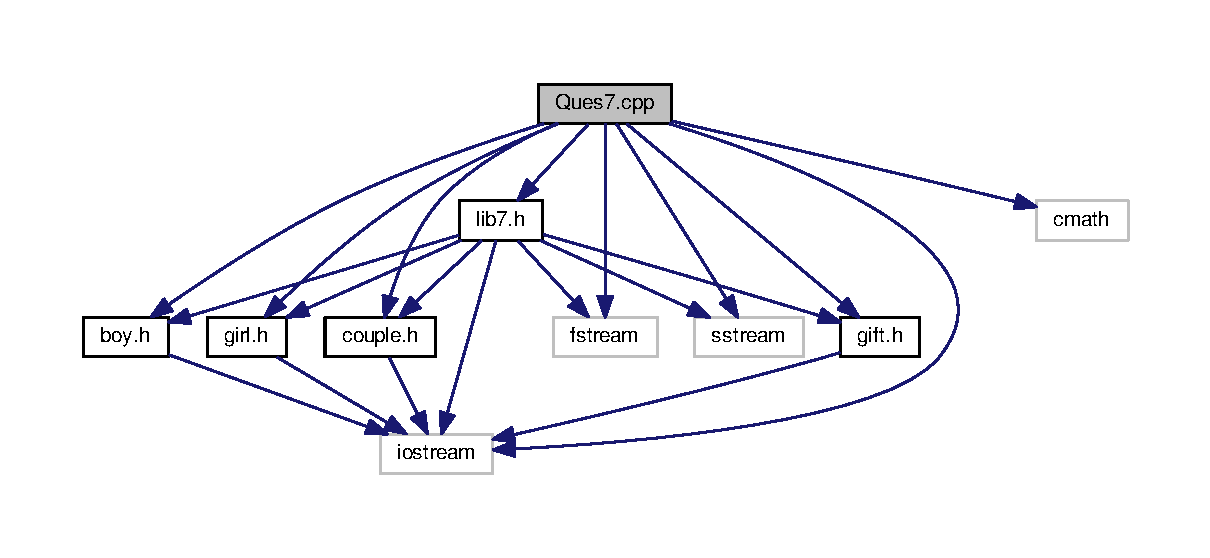
\includegraphics[width=350pt]{Ques7_8cpp__incl}
\end{center}
\end{figure}
\subsection*{Macros}
\begin{DoxyCompactItemize}
\item 
\#define \hyperlink{Ques7_8cpp_a111da81ae5883147168bbb8366377b10}{B}~9
\item 
\#define \hyperlink{Ques7_8cpp_aed9ea78689ecce0b7264c02c7f8a9a54}{G}~5
\item 
\#define \hyperlink{Ques7_8cpp_ac4cf4b2ab929bd23951a8676eeac086b}{C}~5
\item 
\#define \hyperlink{Ques7_8cpp_a5e0c07e523d4e77a2cafca06feb836f6}{Gf}~15
\item 
\#define \hyperlink{Ques7_8cpp_af933676109efed7ab34cea71d748a517}{S}~5
\item 
\#define \hyperlink{Ques7_8cpp_a22995efd1bf00d607d61f25430f44db2}{C\+H\+O\+I\+CE}~2
\end{DoxyCompactItemize}
\subsection*{Functions}
\begin{DoxyCompactItemize}
\item 
void \hyperlink{Ques7_8cpp_ac70f752855ee1cf9ceaa2d749bbad17d}{swap} (\hyperlink{classGift}{Gift} \&a, \hyperlink{classGift}{Gift} \&b)
\item 
void \hyperlink{Ques7_8cpp_a9ed5e5ebda90f206f83cd424ebebe79d}{swapC} (\hyperlink{classCouple}{Couple} \&a, \hyperlink{classCouple}{Couple} \&b)
\item 
int \hyperlink{Ques7_8cpp_ae66f6b31b5ad750f1fe042a706a4e3d4}{main} ()
\end{DoxyCompactItemize}


\subsection{Macro Definition Documentation}
\index{Ques7.\+cpp@{Ques7.\+cpp}!B@{B}}
\index{B@{B}!Ques7.\+cpp@{Ques7.\+cpp}}
\subsubsection[{\texorpdfstring{B}{B}}]{\setlength{\rightskip}{0pt plus 5cm}\#define B~9}\hypertarget{Ques7_8cpp_a111da81ae5883147168bbb8366377b10}{}\label{Ques7_8cpp_a111da81ae5883147168bbb8366377b10}
\index{Ques7.\+cpp@{Ques7.\+cpp}!C@{C}}
\index{C@{C}!Ques7.\+cpp@{Ques7.\+cpp}}
\subsubsection[{\texorpdfstring{C}{C}}]{\setlength{\rightskip}{0pt plus 5cm}\#define C~5}\hypertarget{Ques7_8cpp_ac4cf4b2ab929bd23951a8676eeac086b}{}\label{Ques7_8cpp_ac4cf4b2ab929bd23951a8676eeac086b}
\index{Ques7.\+cpp@{Ques7.\+cpp}!C\+H\+O\+I\+CE@{C\+H\+O\+I\+CE}}
\index{C\+H\+O\+I\+CE@{C\+H\+O\+I\+CE}!Ques7.\+cpp@{Ques7.\+cpp}}
\subsubsection[{\texorpdfstring{C\+H\+O\+I\+CE}{CHOICE}}]{\setlength{\rightskip}{0pt plus 5cm}\#define C\+H\+O\+I\+CE~2}\hypertarget{Ques7_8cpp_a22995efd1bf00d607d61f25430f44db2}{}\label{Ques7_8cpp_a22995efd1bf00d607d61f25430f44db2}
\index{Ques7.\+cpp@{Ques7.\+cpp}!G@{G}}
\index{G@{G}!Ques7.\+cpp@{Ques7.\+cpp}}
\subsubsection[{\texorpdfstring{G}{G}}]{\setlength{\rightskip}{0pt plus 5cm}\#define G~5}\hypertarget{Ques7_8cpp_aed9ea78689ecce0b7264c02c7f8a9a54}{}\label{Ques7_8cpp_aed9ea78689ecce0b7264c02c7f8a9a54}
\index{Ques7.\+cpp@{Ques7.\+cpp}!Gf@{Gf}}
\index{Gf@{Gf}!Ques7.\+cpp@{Ques7.\+cpp}}
\subsubsection[{\texorpdfstring{Gf}{Gf}}]{\setlength{\rightskip}{0pt plus 5cm}\#define Gf~15}\hypertarget{Ques7_8cpp_a5e0c07e523d4e77a2cafca06feb836f6}{}\label{Ques7_8cpp_a5e0c07e523d4e77a2cafca06feb836f6}
\index{Ques7.\+cpp@{Ques7.\+cpp}!S@{S}}
\index{S@{S}!Ques7.\+cpp@{Ques7.\+cpp}}
\subsubsection[{\texorpdfstring{S}{S}}]{\setlength{\rightskip}{0pt plus 5cm}\#define S~5}\hypertarget{Ques7_8cpp_af933676109efed7ab34cea71d748a517}{}\label{Ques7_8cpp_af933676109efed7ab34cea71d748a517}


\subsection{Function Documentation}
\index{Ques7.\+cpp@{Ques7.\+cpp}!main@{main}}
\index{main@{main}!Ques7.\+cpp@{Ques7.\+cpp}}
\subsubsection[{\texorpdfstring{main()}{main()}}]{\setlength{\rightskip}{0pt plus 5cm}int main (
\begin{DoxyParamCaption}
{}
\end{DoxyParamCaption}
)}\hypertarget{Ques7_8cpp_ae66f6b31b5ad750f1fe042a706a4e3d4}{}\label{Ques7_8cpp_ae66f6b31b5ad750f1fe042a706a4e3d4}
taking input from boy.\+dat

taking iput from girl.\+dat

taking input from gift.\+dat

forming couples

printing the couples formed

original couple array

creating hashtables

Sorting couples according to happiness

creating list of boys to be looked for

Selecting algo from library file

for linear search

for binary search

for using hashtable
\begin{DoxyCode}
38 \{
39     \hyperlink{classBoy}{Boy} boys[\hyperlink{Ques7_8cpp_a111da81ae5883147168bbb8366377b10}{B}];
40     \hyperlink{classGirl}{Girl} girls[\hyperlink{Ques7_8cpp_aed9ea78689ecce0b7264c02c7f8a9a54}{G}];
41     \hyperlink{classLibrary}{Library} ob ;
42     \hyperlink{classCouple}{Couple} couples[\hyperlink{Ques7_8cpp_ac4cf4b2ab929bd23951a8676eeac086b}{C}];
43     \hyperlink{classGift}{Gift} gifts[\hyperlink{Ques7_8cpp_a5e0c07e523d4e77a2cafca06feb836f6}{Gf}];
44     
45     \textcolor{keywordtype}{string} line;
46     \textcolor{keywordtype}{int} c = 0, x = 0;
47 
48     ofstream logFile;
49     logFile.open(\textcolor{stringliteral}{"logFile7.dat"});
50 
51 
55     ifstream boyInp(\textcolor{stringliteral}{"boy.dat"});
56     \textcolor{keywordflow}{while}(getline(boyInp,line)) \{
57         \textcolor{keywordflow}{if}(c++ == 0) \textcolor{keywordflow}{continue};
58         istringstream iss(line);
59         \textcolor{keywordtype}{string} name;
60         \textcolor{keywordtype}{int} a,i,b,t,s;
61         \textcolor{keywordtype}{char} ty;
62         \textcolor{keywordflow}{if}((iss>>name>>a>>i>>b>>t>>s>>ty))\{
63             boys[x++].\hyperlink{classBoy_a6ac70867d517f6b429ce67c8eb2915ed}{setDetails}(name,a,i,b,t,s,ty);
64         \} \textcolor{keywordflow}{else} \{
65             \textcolor{keywordflow}{break};
66         \}
67     \}
68 
69     c = 0;
70     x = 0;
74     ifstream girlInp(\textcolor{stringliteral}{"girl.dat"});
75     \textcolor{keywordflow}{while}(getline(girlInp,line)) \{
76         \textcolor{keywordflow}{if}(c++ == 0) \textcolor{keywordflow}{continue};
77         istringstream iss(line);
78         \textcolor{keywordtype}{string} name;
79         \textcolor{keywordtype}{int} a,i,m,s;
80         \textcolor{keywordtype}{char} ty,cr;
81         \textcolor{keywordflow}{if}((iss>>name>>a>>i>>m>>cr>>s>>ty))\{
82             girls[x++].\hyperlink{classGirl_a4bff314dba17278eb1093b15f7be80bd}{setDetails}(name,a,i,m,ty,s,cr);
83         \} \textcolor{keywordflow}{else} \{
84             \textcolor{keywordflow}{break};
85         \}
86     \}
87 
88     c = 0;
89     x = 0;
93     ifstream giftInp(\textcolor{stringliteral}{"gift.dat"});
94     \textcolor{keywordflow}{while}(getline(giftInp,line)) \{
95         \textcolor{keywordflow}{if}(c++ == 0) \textcolor{keywordflow}{continue};
96         istringstream iss(line);
97         \textcolor{keywordtype}{int} id,p,v;
98         \textcolor{keywordtype}{char} ty;
99         \textcolor{keywordflow}{if}((iss>>\textcolor{keywordtype}{id}>>p>>ty>>v))\{
100             gifts[x++].\hyperlink{classGift_abc74fbed8b31b5bb7745b3e0c934da9e}{setDetail}(\textcolor{keywordtype}{id},p,ty,0);
101         \} \textcolor{keywordflow}{else} \{
102             \textcolor{keywordflow}{break};
103         \}
104     \}
105     
106     c = 0;
110     \textcolor{keywordflow}{for}(\textcolor{keywordtype}{int} i = 0 ; i < \hyperlink{Ques7_8cpp_aed9ea78689ecce0b7264c02c7f8a9a54}{G}; i++) \{
111         \textcolor{keywordflow}{if}(girls[i].getCriterion() == \textcolor{charliteral}{'A'}) \{
112             \textcolor{keywordtype}{int} max= -99;
113             \textcolor{keywordtype}{int} ind = -1;
114             \textcolor{keywordflow}{for}(\textcolor{keywordtype}{int} j = 0; j < \hyperlink{Ques7_8cpp_a111da81ae5883147168bbb8366377b10}{B}; j++) \{
115                 \textcolor{keywordflow}{if}(boys[j].getAttractiveness() > max && boys[j].getStatus() == 0) \{
116                     \textcolor{keywordflow}{if}(boys[j].getBudget() > girls[i].getMaintenance()) \{
117                         \textcolor{keywordflow}{if}(girls[i].getAttractiveness() > boys[j].getThreshold()) \{
118                             max = boys[j].\hyperlink{classBoy_a814ef4919f2ac86c6ee70f9698afad3d}{getAttractiveness}();
119                             ind = j;
120                         \}
121                     \}
122                 \}
123             \}
124         
125             \textcolor{keywordflow}{if}(ind != -1) \{
126                 boys[ind].\hyperlink{classBoy_a3d29dcc4137fbfc0306cbd7df82781c3}{setStatus}(1);
127                 girls[i].\hyperlink{classGirl_a201527323b3fabac4b089f003b8fcc4a}{setStatus}(1);
128                 couples[c++].\hyperlink{classCouple_a0057d3dfd3939a156cd99f6c5cf32279}{setDetails}(boys[ind].getName(),girls[i].getname()) ; 
129             \}       
130         \} \textcolor{keywordflow}{else} \textcolor{keywordflow}{if}(girls[i].getCriterion() == \textcolor{charliteral}{'I'}) \{
131             \textcolor{keywordtype}{int} max= -99;
132                         \textcolor{keywordtype}{int} ind = -1;
133                         \textcolor{keywordflow}{for}(\textcolor{keywordtype}{int} j = 0; j < \hyperlink{Ques7_8cpp_a111da81ae5883147168bbb8366377b10}{B}; j++) \{
134                                 \textcolor{keywordflow}{if}(boys[j].getIntelligence() > max && boys[j].getStatus() == 0) \{
135                                         \textcolor{keywordflow}{if}(boys[j].getBudget() > girls[i].getMaintenance()) \{
136                                                 \textcolor{keywordflow}{if}(girls[i].getAttractiveness() > boys[j].getThreshold()) \{
137                                                         max = boys[j].
      \hyperlink{classBoy_ad52c9e04ab591f3909d2342d6cae0168}{getIntelligence}();
138                                                         ind = j;
139                                                 \}
140                                         \}
141                                 \}
142                         \}
143                           
144                         \textcolor{keywordflow}{if}(ind != -1) \{
145                                 boys[ind].\hyperlink{classBoy_a3d29dcc4137fbfc0306cbd7df82781c3}{setStatus}(1);
146                                 girls[i].\hyperlink{classGirl_a201527323b3fabac4b089f003b8fcc4a}{setStatus}(1);
147                                 couples[c++].\hyperlink{classCouple_a0057d3dfd3939a156cd99f6c5cf32279}{setDetails}(boys[ind].getName(),girls[i].getname()) ;
148                         \}
149 
150         \} \textcolor{keywordflow}{else} \{
151             \textcolor{keywordtype}{int} max= -99;
152                         \textcolor{keywordtype}{int} ind = -1;
153                         \textcolor{keywordflow}{for}(\textcolor{keywordtype}{int} j = 0; j < \hyperlink{Ques7_8cpp_a111da81ae5883147168bbb8366377b10}{B}; j++) \{
154                                 \textcolor{keywordflow}{if}(boys[j].getBudget() > max && boys[j].getStatus() == 0) \{
155                                         \textcolor{keywordflow}{if}(boys[j].getBudget() > girls[i].getMaintenance()) \{
156                                                 \textcolor{keywordflow}{if}(girls[i].getAttractiveness() > boys[j].getThreshold()) \{
157                                                         max = boys[j].\hyperlink{classBoy_a05c48b12091ebcad44ba86ba88514ac5}{getBudget}();
158                                                         ind = j;
159                                                 \}
160                                         \}
161                                 \}
162                         \}
163                           
164                         \textcolor{keywordflow}{if}(ind != -1) \{
165                                 boys[ind].\hyperlink{classBoy_a3d29dcc4137fbfc0306cbd7df82781c3}{setStatus}(1);
166                                 girls[i].\hyperlink{classGirl_a201527323b3fabac4b089f003b8fcc4a}{setStatus}(1);
167                                 couples[c++].\hyperlink{classCouple_a0057d3dfd3939a156cd99f6c5cf32279}{setDetails}(boys[ind].getName(),girls[i].getname()) ;
168                         \}
169             
170         \}
171     \}
172 
176     logFile<<\textcolor{stringliteral}{"-----------------COUPLES-------------------\(\backslash\)n\(\backslash\)n"};
177     \textcolor{keywordflow}{for}(\textcolor{keywordtype}{int} i = 0 ;i < \hyperlink{Ques7_8cpp_ac4cf4b2ab929bd23951a8676eeac086b}{C}; i++) \{
178         logFile<<\textcolor{stringliteral}{"Boy b"}<<couples[i].\hyperlink{classCouple_a092cbc580ea255febc3eb211c5f56512}{getBoy}()<<\textcolor{stringliteral}{" and Girl g"}<<couples[i].
      \hyperlink{classCouple_a653983df7e331c0534ae2ce42e9856c5}{getGirl}()<<\textcolor{stringliteral}{"\(\backslash\)n"};
179         
180     \}
181 
185     ob.\hyperlink{classLibrary_a37cc785266d6a6aeb820499ba875cef1}{couples} = couples;
186 
190     \textcolor{keywordflow}{for}(\textcolor{keywordtype}{int} i = 0; i < C-1; i++) \{
191         ob.\hyperlink{classLibrary_a81e01bd9f8b2f1fdbc3420b71de2dc49}{hashCouples}[i].\hyperlink{classCouple_a0057d3dfd3939a156cd99f6c5cf32279}{setDetails}(\textcolor{stringliteral}{""},\textcolor{stringliteral}{""}) ;
192     \}
193     \textcolor{keywordflow}{for}(\textcolor{keywordtype}{int} i = 0; i < \hyperlink{Ques7_8cpp_ac4cf4b2ab929bd23951a8676eeac086b}{C}; i++) \{
194         \textcolor{keywordtype}{int} ind = (couples[i].\hyperlink{classCouple_a092cbc580ea255febc3eb211c5f56512}{getBoy}()[0] + 7)%C;
195         \textcolor{keywordflow}{while}(ob.\hyperlink{classLibrary_a81e01bd9f8b2f1fdbc3420b71de2dc49}{hashCouples}[ind].\hyperlink{classCouple_a092cbc580ea255febc3eb211c5f56512}{getBoy}() != \textcolor{stringliteral}{""}) ind = (ind+1)%
      \hyperlink{Ques7_8cpp_ac4cf4b2ab929bd23951a8676eeac086b}{C};
196         ob.\hyperlink{classLibrary_a81e01bd9f8b2f1fdbc3420b71de2dc49}{hashCouples}[ind] = couples[i]; 
197     \}
198 
202         \textcolor{keywordflow}{for}(\textcolor{keywordtype}{int} i = 0  ; i< C-1; i++) \{
203             \textcolor{keywordflow}{for}(\textcolor{keywordtype}{int} j = i+1; j < \hyperlink{Ques7_8cpp_ac4cf4b2ab929bd23951a8676eeac086b}{C}; j++) \{
204                 \textcolor{keywordflow}{if}(couples[i].getBoy()[0] > couples[j].\hyperlink{classCouple_a092cbc580ea255febc3eb211c5f56512}{getBoy}()[0]) \{
205                     \hyperlink{Ques7_8cpp_a9ed5e5ebda90f206f83cd424ebebe79d}{swapC}(couples[i],couples[j]);
206                 \}   
207             \}
208         \}
209     ob.\hyperlink{classLibrary_ac22a9d065ab96fcb3d44e203725e6de6}{sortedCouples} = couples;
210 
214     logFile<<\textcolor{stringliteral}{"\(\backslash\)n-----------List of Boys----------\(\backslash\)n\(\backslash\)n"};
215     \textcolor{keywordflow}{for}(\textcolor{keywordtype}{int} i = 0; i < \hyperlink{Ques7_8cpp_af933676109efed7ab34cea71d748a517}{S}; i++) \{
216         ob.\hyperlink{classLibrary_a28fd1fddb9c961b2cfbb4a054f1ab258}{boysList}[i]= boys[i];    
217         logFile<<\textcolor{stringliteral}{"b"}<<ob.\hyperlink{classLibrary_a28fd1fddb9c961b2cfbb4a054f1ab258}{boysList}[i].\hyperlink{classBoy_a53e90a641c928c0849e33eca847e902d}{getName}()<<\textcolor{stringliteral}{" "};
218     \}   
219     logFile<<endl;
220 
224     \textcolor{keywordtype}{int} choice = \hyperlink{Ques7_8cpp_a22995efd1bf00d607d61f25430f44db2}{CHOICE};
225     \textcolor{keywordflow}{switch}(choice) \{
226         \textcolor{keywordflow}{case} 1:     
230             ob.\hyperlink{classLibrary_af9853cceb7af37b77091c3330b532b2f}{searchArr}();
231             \textcolor{keywordflow}{break};
232         \textcolor{keywordflow}{case} 2:     
236             ob.\hyperlink{classLibrary_a835ea2c0b31c569aac4a406843c55254}{searchSortedArr}();
237             \textcolor{keywordflow}{break};
238         \textcolor{keywordflow}{case} 3:     
242             cout<<choice<<endl;
243             ob.\hyperlink{classLibrary_ad14b4301aa6279c13408ff948ca4fd6a}{searchHash}();
244             \textcolor{keywordflow}{break};
245 
246     \}
247     logFile.close();
248 \}
\end{DoxyCode}
\index{Ques7.\+cpp@{Ques7.\+cpp}!swap@{swap}}
\index{swap@{swap}!Ques7.\+cpp@{Ques7.\+cpp}}
\subsubsection[{\texorpdfstring{swap(\+Gift \&a, Gift \&b)}{swap(Gift &a, Gift &b)}}]{\setlength{\rightskip}{0pt plus 5cm}void swap (
\begin{DoxyParamCaption}
\item[{{\bf Gift} \&}]{a, }
\item[{{\bf Gift} \&}]{b}
\end{DoxyParamCaption}
)}\hypertarget{Ques7_8cpp_ac70f752855ee1cf9ceaa2d749bbad17d}{}\label{Ques7_8cpp_ac70f752855ee1cf9ceaa2d749bbad17d}

\begin{DoxyCode}
23 \{
24     \hyperlink{classGift}{Gift} temp = a;
25     a = b;
26     b = temp;
27 \}
\end{DoxyCode}
\index{Ques7.\+cpp@{Ques7.\+cpp}!swapC@{swapC}}
\index{swapC@{swapC}!Ques7.\+cpp@{Ques7.\+cpp}}
\subsubsection[{\texorpdfstring{swap\+C(\+Couple \&a, Couple \&b)}{swapC(Couple &a, Couple &b)}}]{\setlength{\rightskip}{0pt plus 5cm}void swapC (
\begin{DoxyParamCaption}
\item[{{\bf Couple} \&}]{a, }
\item[{{\bf Couple} \&}]{b}
\end{DoxyParamCaption}
)}\hypertarget{Ques7_8cpp_a9ed5e5ebda90f206f83cd424ebebe79d}{}\label{Ques7_8cpp_a9ed5e5ebda90f206f83cd424ebebe79d}

\begin{DoxyCode}
30 \{
31     \hyperlink{classCouple}{Couple} temp = a;
32     a = b;
33     b = temp;
34 \}
\end{DoxyCode}

\hypertarget{Ques8_8cpp}{}\section{Ques8.\+cpp File Reference}
\label{Ques8_8cpp}\index{Ques8.\+cpp@{Ques8.\+cpp}}
{\ttfamily \#include $<$iostream$>$}\\*
{\ttfamily \#include $<$fstream$>$}\\*
{\ttfamily \#include $<$sstream$>$}\\*
{\ttfamily \#include $<$cmath$>$}\\*
{\ttfamily \#include \char`\"{}boy.\+h\char`\"{}}\\*
{\ttfamily \#include \char`\"{}girl.\+h\char`\"{}}\\*
{\ttfamily \#include \char`\"{}couple.\+h\char`\"{}}\\*
{\ttfamily \#include \char`\"{}gift.\+h\char`\"{}}\\*
{\ttfamily \#include \char`\"{}lib8.\+h\char`\"{}}\\*
Include dependency graph for Ques8.\+cpp\+:
\nopagebreak
\begin{figure}[H]
\begin{center}
\leavevmode
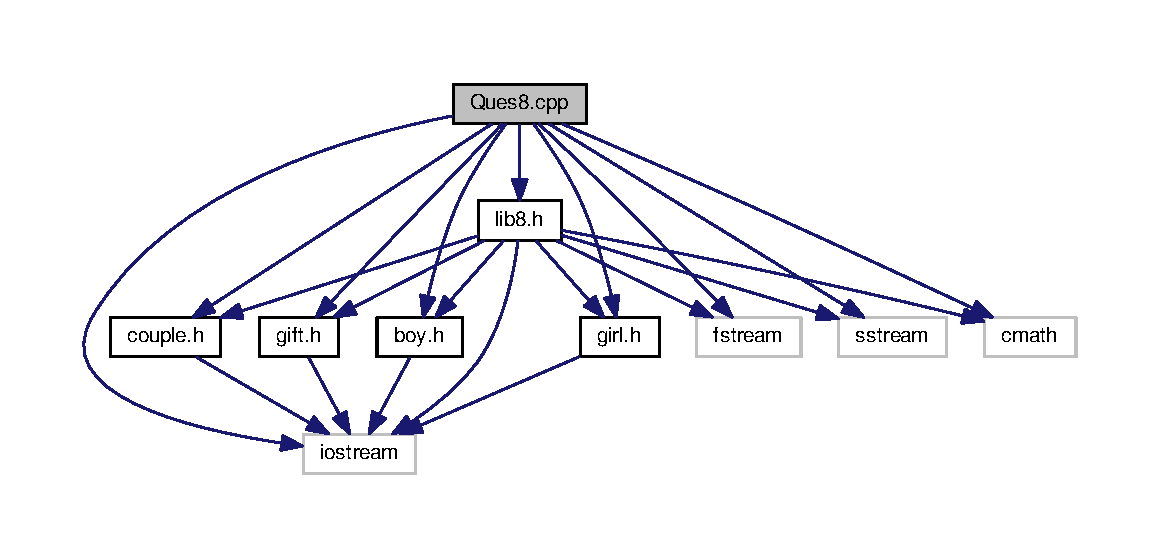
\includegraphics[width=350pt]{Ques8_8cpp__incl}
\end{center}
\end{figure}
\subsection*{Macros}
\begin{DoxyCompactItemize}
\item 
\#define \hyperlink{Ques8_8cpp_a111da81ae5883147168bbb8366377b10}{B}~9
\item 
\#define \hyperlink{Ques8_8cpp_aed9ea78689ecce0b7264c02c7f8a9a54}{G}~5
\item 
\#define \hyperlink{Ques8_8cpp_ac4cf4b2ab929bd23951a8676eeac086b}{C}~5
\item 
\#define \hyperlink{Ques8_8cpp_a5e0c07e523d4e77a2cafca06feb836f6}{Gf}~15
\item 
\#define \hyperlink{Ques8_8cpp_a97d832ae23af4f215e801e37e4f94254}{K}~2
\item 
\#define \hyperlink{Ques8_8cpp_a22995efd1bf00d607d61f25430f44db2}{C\+H\+O\+I\+CE}~2
\end{DoxyCompactItemize}
\subsection*{Functions}
\begin{DoxyCompactItemize}
\item 
void \hyperlink{Ques8_8cpp_a9ed5e5ebda90f206f83cd424ebebe79d}{swapC} (\hyperlink{classCouple}{Couple} \&a, \hyperlink{classCouple}{Couple} \&b)
\item 
int \hyperlink{Ques8_8cpp_ae66f6b31b5ad750f1fe042a706a4e3d4}{main} ()
\end{DoxyCompactItemize}


\subsection{Macro Definition Documentation}
\index{Ques8.\+cpp@{Ques8.\+cpp}!B@{B}}
\index{B@{B}!Ques8.\+cpp@{Ques8.\+cpp}}
\subsubsection[{\texorpdfstring{B}{B}}]{\setlength{\rightskip}{0pt plus 5cm}\#define B~9}\hypertarget{Ques8_8cpp_a111da81ae5883147168bbb8366377b10}{}\label{Ques8_8cpp_a111da81ae5883147168bbb8366377b10}
\index{Ques8.\+cpp@{Ques8.\+cpp}!C@{C}}
\index{C@{C}!Ques8.\+cpp@{Ques8.\+cpp}}
\subsubsection[{\texorpdfstring{C}{C}}]{\setlength{\rightskip}{0pt plus 5cm}\#define C~5}\hypertarget{Ques8_8cpp_ac4cf4b2ab929bd23951a8676eeac086b}{}\label{Ques8_8cpp_ac4cf4b2ab929bd23951a8676eeac086b}
\index{Ques8.\+cpp@{Ques8.\+cpp}!C\+H\+O\+I\+CE@{C\+H\+O\+I\+CE}}
\index{C\+H\+O\+I\+CE@{C\+H\+O\+I\+CE}!Ques8.\+cpp@{Ques8.\+cpp}}
\subsubsection[{\texorpdfstring{C\+H\+O\+I\+CE}{CHOICE}}]{\setlength{\rightskip}{0pt plus 5cm}\#define C\+H\+O\+I\+CE~2}\hypertarget{Ques8_8cpp_a22995efd1bf00d607d61f25430f44db2}{}\label{Ques8_8cpp_a22995efd1bf00d607d61f25430f44db2}
\index{Ques8.\+cpp@{Ques8.\+cpp}!G@{G}}
\index{G@{G}!Ques8.\+cpp@{Ques8.\+cpp}}
\subsubsection[{\texorpdfstring{G}{G}}]{\setlength{\rightskip}{0pt plus 5cm}\#define G~5}\hypertarget{Ques8_8cpp_aed9ea78689ecce0b7264c02c7f8a9a54}{}\label{Ques8_8cpp_aed9ea78689ecce0b7264c02c7f8a9a54}
\index{Ques8.\+cpp@{Ques8.\+cpp}!Gf@{Gf}}
\index{Gf@{Gf}!Ques8.\+cpp@{Ques8.\+cpp}}
\subsubsection[{\texorpdfstring{Gf}{Gf}}]{\setlength{\rightskip}{0pt plus 5cm}\#define Gf~15}\hypertarget{Ques8_8cpp_a5e0c07e523d4e77a2cafca06feb836f6}{}\label{Ques8_8cpp_a5e0c07e523d4e77a2cafca06feb836f6}
\index{Ques8.\+cpp@{Ques8.\+cpp}!K@{K}}
\index{K@{K}!Ques8.\+cpp@{Ques8.\+cpp}}
\subsubsection[{\texorpdfstring{K}{K}}]{\setlength{\rightskip}{0pt plus 5cm}\#define K~2}\hypertarget{Ques8_8cpp_a97d832ae23af4f215e801e37e4f94254}{}\label{Ques8_8cpp_a97d832ae23af4f215e801e37e4f94254}


\subsection{Function Documentation}
\index{Ques8.\+cpp@{Ques8.\+cpp}!main@{main}}
\index{main@{main}!Ques8.\+cpp@{Ques8.\+cpp}}
\subsubsection[{\texorpdfstring{main()}{main()}}]{\setlength{\rightskip}{0pt plus 5cm}int main (
\begin{DoxyParamCaption}
{}
\end{DoxyParamCaption}
)}\hypertarget{Ques8_8cpp_ae66f6b31b5ad750f1fe042a706a4e3d4}{}\label{Ques8_8cpp_ae66f6b31b5ad750f1fe042a706a4e3d4}
taking input from boy.\+dat

taking input from girl.\+dat

forming couples

printing couples
\begin{DoxyCode}
31 \{
32     \hyperlink{classBoy}{Boy} boys[\hyperlink{Ques8_8cpp_a111da81ae5883147168bbb8366377b10}{B}];
33     \hyperlink{classGirl}{Girl} girls[\hyperlink{Ques8_8cpp_aed9ea78689ecce0b7264c02c7f8a9a54}{G}];
34     \hyperlink{classCouple}{Couple} couples[\hyperlink{Ques8_8cpp_ac4cf4b2ab929bd23951a8676eeac086b}{C}];
35     \hyperlink{classGift}{Gift} gifts[\hyperlink{Ques8_8cpp_a5e0c07e523d4e77a2cafca06feb836f6}{Gf}];
36 
37     
38     \textcolor{keywordtype}{string} line;
39     \textcolor{keywordtype}{int} c = 0, x = 0;
40 
41     ofstream logFile;
42     logFile.open(\textcolor{stringliteral}{"logFile8.dat"});
43 
44 
48     ifstream boyInp(\textcolor{stringliteral}{"boy.dat"});
49     \textcolor{keywordflow}{while}(getline(boyInp,line)) \{
50         \textcolor{keywordflow}{if}(c++ == 0) \textcolor{keywordflow}{continue};
51         istringstream iss(line);
52         \textcolor{keywordtype}{string} name;
53         \textcolor{keywordtype}{int} a,i,b,t,s;
54         \textcolor{keywordtype}{char} ty;
55         \textcolor{keywordflow}{if}((iss>>name>>a>>i>>b>>t>>s>>ty))\{
56             boys[x++].\hyperlink{classBoy_a6ac70867d517f6b429ce67c8eb2915ed}{setDetails}(name,a,i,b,t,s,ty);
57         \} \textcolor{keywordflow}{else} \{
58             \textcolor{keywordflow}{break};
59         \}
60     \}
61 
62     c = 0;
63     x = 0;
67     ifstream girlInp(\textcolor{stringliteral}{"girl.dat"});
68     \textcolor{keywordflow}{while}(getline(girlInp,line)) \{
69         \textcolor{keywordflow}{if}(c++ == 0) \textcolor{keywordflow}{continue};
70         istringstream iss(line);
71         \textcolor{keywordtype}{string} name;
72         \textcolor{keywordtype}{int} a,i,m,s;
73         \textcolor{keywordtype}{char} ty,cr;
74         \textcolor{keywordflow}{if}((iss>>name>>a>>i>>m>>cr>>s>>ty))\{
75             girls[x++].\hyperlink{classGirl_a4bff314dba17278eb1093b15f7be80bd}{setDetails}(name,a,i,m,ty,s,cr);
76         \} \textcolor{keywordflow}{else} \{
77             \textcolor{keywordflow}{break};
78         \}
79     \}
80 
81     
82     
83     c = 0;
87     \textcolor{keywordflow}{for}(\textcolor{keywordtype}{int} i = 0 ; i < \hyperlink{Ques8_8cpp_aed9ea78689ecce0b7264c02c7f8a9a54}{G}; i++) \{
88         \textcolor{keywordflow}{if}(girls[i].getCriterion() == \textcolor{charliteral}{'A'}) \{
89             \textcolor{keywordtype}{int} max= -99;
90             \textcolor{keywordtype}{int} ind = -1;
91             \textcolor{keywordflow}{for}(\textcolor{keywordtype}{int} j = 0; j < \hyperlink{Ques8_8cpp_a111da81ae5883147168bbb8366377b10}{B}; j++) \{
92                 \textcolor{keywordflow}{if}(boys[j].getAttractiveness() > max && boys[j].getStatus() == 0) \{
93                     \textcolor{keywordflow}{if}(boys[j].getBudget() > girls[i].getMaintenance()) \{
94                         \textcolor{keywordflow}{if}(girls[i].getAttractiveness() > boys[j].getThreshold()) \{
95                             max = boys[j].\hyperlink{classBoy_a814ef4919f2ac86c6ee70f9698afad3d}{getAttractiveness}();
96                             ind = j;
97                         \}
98                     \}
99                 \}
100             \}
101         
102             \textcolor{keywordflow}{if}(ind != -1) \{
103                 boys[ind].\hyperlink{classBoy_a3d29dcc4137fbfc0306cbd7df82781c3}{setStatus}(1);
104                 girls[i].\hyperlink{classGirl_a201527323b3fabac4b089f003b8fcc4a}{setStatus}(1);
105                 couples[c++].\hyperlink{classCouple_a0057d3dfd3939a156cd99f6c5cf32279}{setDetails}(boys[ind].getName(),girls[i].getname()) ; 
106             \}       
107         \} \textcolor{keywordflow}{else} \textcolor{keywordflow}{if}(girls[i].getCriterion() == \textcolor{charliteral}{'I'}) \{
108             \textcolor{keywordtype}{int} max= -99;
109                         \textcolor{keywordtype}{int} ind = -1;
110                         \textcolor{keywordflow}{for}(\textcolor{keywordtype}{int} j = 0; j < \hyperlink{Ques8_8cpp_a111da81ae5883147168bbb8366377b10}{B}; j++) \{
111                                 \textcolor{keywordflow}{if}(boys[j].getIntelligence() > max && boys[j].getStatus() == 0) \{
112                                         \textcolor{keywordflow}{if}(boys[j].getBudget() > girls[i].getMaintenance()) \{
113                                                 \textcolor{keywordflow}{if}(girls[i].getAttractiveness() > boys[j].getThreshold()) \{
114                                                         max = boys[j].
      \hyperlink{classBoy_ad52c9e04ab591f3909d2342d6cae0168}{getIntelligence}();
115                                                         ind = j;
116                                                 \}
117                                         \}
118                                 \}
119                         \}
120                           
121                         \textcolor{keywordflow}{if}(ind != -1) \{
122                                 boys[ind].\hyperlink{classBoy_a3d29dcc4137fbfc0306cbd7df82781c3}{setStatus}(1);
123                                 girls[i].\hyperlink{classGirl_a201527323b3fabac4b089f003b8fcc4a}{setStatus}(1);
124                                 couples[c++].\hyperlink{classCouple_a0057d3dfd3939a156cd99f6c5cf32279}{setDetails}(boys[ind].getName(),girls[i].getname()) ;
125                         \}
126 
127         \} \textcolor{keywordflow}{else} \{
128             \textcolor{keywordtype}{int} max= -99;
129                         \textcolor{keywordtype}{int} ind = -1;
130                         \textcolor{keywordflow}{for}(\textcolor{keywordtype}{int} j = 0; j < \hyperlink{Ques8_8cpp_a111da81ae5883147168bbb8366377b10}{B}; j++) \{
131                                 \textcolor{keywordflow}{if}(boys[j].getBudget() > max && boys[j].getStatus() == 0) \{
132                                         \textcolor{keywordflow}{if}(boys[j].getBudget() > girls[i].getMaintenance()) \{
133                                                 \textcolor{keywordflow}{if}(girls[i].getAttractiveness() > boys[j].getThreshold()) \{
134                                                         max = boys[j].\hyperlink{classBoy_a05c48b12091ebcad44ba86ba88514ac5}{getBudget}();
135                                                         ind = j;
136                                                 \}
137                                         \}
138                                 \}
139                         \}
140                           
141                         \textcolor{keywordflow}{if}(ind != -1) \{
142                                 boys[ind].\hyperlink{classBoy_a3d29dcc4137fbfc0306cbd7df82781c3}{setStatus}(1);
143                                 girls[i].\hyperlink{classGirl_a201527323b3fabac4b089f003b8fcc4a}{setStatus}(1);
144                                 couples[c++].\hyperlink{classCouple_a0057d3dfd3939a156cd99f6c5cf32279}{setDetails}(boys[ind].getName(),girls[i].getname()) ;
145                         \}
146             
147         \}
148     \}
149 
153     logFile<<\textcolor{stringliteral}{"-----------------COUPLES-------------------\(\backslash\)n\(\backslash\)n"};
154 
155     \textcolor{keywordflow}{for}(\textcolor{keywordtype}{int} i = 0 ;i < \hyperlink{Ques8_8cpp_ac4cf4b2ab929bd23951a8676eeac086b}{C}; i++) \{
156         logFile<<\textcolor{stringliteral}{"Boy b"}<<couples[i].\hyperlink{classCouple_a092cbc580ea255febc3eb211c5f56512}{getBoy}()<<\textcolor{stringliteral}{" and Girl g"}<<couples[i].
      \hyperlink{classCouple_a653983df7e331c0534ae2ce42e9856c5}{getGirl}()<<\textcolor{stringliteral}{"\(\backslash\)n"};
157         
158     \}
159     logFile<<endl;
160 
161 
162     \hyperlink{classGiftAllocation}{GiftAllocation} * ob;
163         
164     \textcolor{keywordtype}{int} choice = \hyperlink{Ques8_8cpp_a22995efd1bf00d607d61f25430f44db2}{CHOICE};
165     
166     \textcolor{keywordflow}{switch}(choice) \{
167         \textcolor{keywordflow}{case} 1:     \textcolor{comment}{//for choosing method1}
168             \hyperlink{classmethod1}{method1} m1;
169             
170             ob = &m1;
171 
172             \textcolor{comment}{//taking input for gifts}
173             ob->\hyperlink{classGiftAllocation_a251311eacec6f50e78300c576b3938b9}{takeInput}();
174 
175             \textcolor{comment}{//sorting gifts }
176             ob->\hyperlink{classGiftAllocation_a54ab23085223d306af9aa3ded70901be}{sortingGifts}();
177             m1.\hyperlink{classmethod1_a8f2ac4501ad63e68065236359e368864}{allocate}(couples,boys,girls);
178             logFile<<\textcolor{stringliteral}{"-----------------YOU CHOSE METHOD 1-------------------"}<<endl;
179             ob->\hyperlink{classGiftAllocation_a9ea227b1d051645d9aa54d7c4d4d0ce3}{printingGifts}(couples);
180             \textcolor{keywordflow}{break};
181 
182         \textcolor{keywordflow}{case} 2:     \textcolor{comment}{//for choosing method2}
183             \hyperlink{classmethod2}{method2} m2;
184             ob = &m2;   \textcolor{comment}{//upcasting}
185             \textcolor{comment}{//taking input for gifts}
186             ob->\hyperlink{classGiftAllocation_a251311eacec6f50e78300c576b3938b9}{takeInput}();
187 
188             \textcolor{comment}{//sorting gifts }
189             ob->\hyperlink{classGiftAllocation_a54ab23085223d306af9aa3ded70901be}{sortingGifts}();
190             m2.\hyperlink{classmethod2_af5e7e4483c463a9e13a731d7d56a99f1}{allocate}(couples,boys,girls);
191             logFile<<\textcolor{stringliteral}{"-----------------YOU CHOSE METHOD 2-------------------"}<<endl;
192             ob->\hyperlink{classGiftAllocation_a9ea227b1d051645d9aa54d7c4d4d0ce3}{printingGifts}(couples);
193             \textcolor{keywordflow}{break};
194         
195     \}
196 
197 
198 
199     
200     
201 
202     
203     
204 
205     logFile.close();
206 \}
\end{DoxyCode}
\index{Ques8.\+cpp@{Ques8.\+cpp}!swapC@{swapC}}
\index{swapC@{swapC}!Ques8.\+cpp@{Ques8.\+cpp}}
\subsubsection[{\texorpdfstring{swap\+C(\+Couple \&a, Couple \&b)}{swapC(Couple &a, Couple &b)}}]{\setlength{\rightskip}{0pt plus 5cm}void swapC (
\begin{DoxyParamCaption}
\item[{{\bf Couple} \&}]{a, }
\item[{{\bf Couple} \&}]{b}
\end{DoxyParamCaption}
)}\hypertarget{Ques8_8cpp_a9ed5e5ebda90f206f83cd424ebebe79d}{}\label{Ques8_8cpp_a9ed5e5ebda90f206f83cd424ebebe79d}

\begin{DoxyCode}
23 \{
24     \hyperlink{classCouple}{Couple} temp = a;
25     a = b;
26     b = temp;
27 \}
\end{DoxyCode}

\hypertarget{Ques9_8cpp}{}\section{Ques9.\+cpp File Reference}
\label{Ques9_8cpp}\index{Ques9.\+cpp@{Ques9.\+cpp}}
{\ttfamily \#include $<$iostream$>$}\\*
{\ttfamily \#include $<$fstream$>$}\\*
{\ttfamily \#include $<$sstream$>$}\\*
{\ttfamily \#include $<$cmath$>$}\\*
{\ttfamily \#include \char`\"{}boy.\+h\char`\"{}}\\*
{\ttfamily \#include \char`\"{}girl.\+h\char`\"{}}\\*
{\ttfamily \#include \char`\"{}couple.\+h\char`\"{}}\\*
{\ttfamily \#include \char`\"{}gift.\+h\char`\"{}}\\*
Include dependency graph for Ques9.\+cpp\+:
\nopagebreak
\begin{figure}[H]
\begin{center}
\leavevmode
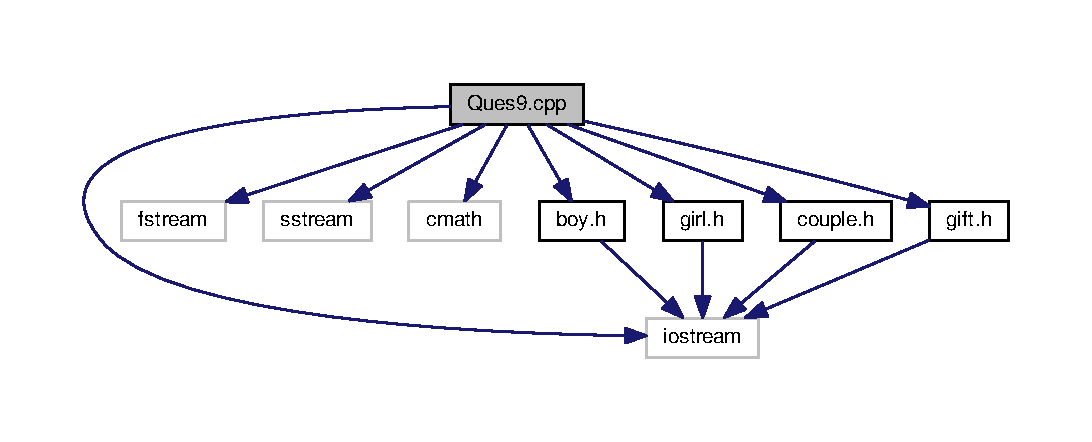
\includegraphics[width=350pt]{Ques9_8cpp__incl}
\end{center}
\end{figure}
\subsection*{Macros}
\begin{DoxyCompactItemize}
\item 
\#define \hyperlink{Ques9_8cpp_a111da81ae5883147168bbb8366377b10}{B}~9
\item 
\#define \hyperlink{Ques9_8cpp_aed9ea78689ecce0b7264c02c7f8a9a54}{G}~5
\item 
\#define \hyperlink{Ques9_8cpp_ac4cf4b2ab929bd23951a8676eeac086b}{C}~5
\item 
\#define \hyperlink{Ques9_8cpp_a5e0c07e523d4e77a2cafca06feb836f6}{Gf}~15
\item 
\#define \hyperlink{Ques9_8cpp_a97d832ae23af4f215e801e37e4f94254}{K}~2
\end{DoxyCompactItemize}
\subsection*{Functions}
\begin{DoxyCompactItemize}
\item 
void \hyperlink{Ques9_8cpp_ac70f752855ee1cf9ceaa2d749bbad17d}{swap} (\hyperlink{classGift}{Gift} \&a, \hyperlink{classGift}{Gift} \&b)
\item 
void \hyperlink{Ques9_8cpp_a9ed5e5ebda90f206f83cd424ebebe79d}{swapC} (\hyperlink{classCouple}{Couple} \&a, \hyperlink{classCouple}{Couple} \&b)
\item 
{\footnotesize template$<$class T $>$ }\\void \hyperlink{Ques9_8cpp_afb2bbadfe7cfd2620d67ca6d0ccb2411}{sorting\+Datastructure} (\hyperlink{Ques6_8cpp_a0acb682b8260ab1c60b918599864e2e5}{T} $\ast$arr, int n, int k, string s)
\item 
int \hyperlink{Ques9_8cpp_ae66f6b31b5ad750f1fe042a706a4e3d4}{main} ()
\end{DoxyCompactItemize}


\subsection{Macro Definition Documentation}
\index{Ques9.\+cpp@{Ques9.\+cpp}!B@{B}}
\index{B@{B}!Ques9.\+cpp@{Ques9.\+cpp}}
\subsubsection[{\texorpdfstring{B}{B}}]{\setlength{\rightskip}{0pt plus 5cm}\#define B~9}\hypertarget{Ques9_8cpp_a111da81ae5883147168bbb8366377b10}{}\label{Ques9_8cpp_a111da81ae5883147168bbb8366377b10}
\index{Ques9.\+cpp@{Ques9.\+cpp}!C@{C}}
\index{C@{C}!Ques9.\+cpp@{Ques9.\+cpp}}
\subsubsection[{\texorpdfstring{C}{C}}]{\setlength{\rightskip}{0pt plus 5cm}\#define C~5}\hypertarget{Ques9_8cpp_ac4cf4b2ab929bd23951a8676eeac086b}{}\label{Ques9_8cpp_ac4cf4b2ab929bd23951a8676eeac086b}
\index{Ques9.\+cpp@{Ques9.\+cpp}!G@{G}}
\index{G@{G}!Ques9.\+cpp@{Ques9.\+cpp}}
\subsubsection[{\texorpdfstring{G}{G}}]{\setlength{\rightskip}{0pt plus 5cm}\#define G~5}\hypertarget{Ques9_8cpp_aed9ea78689ecce0b7264c02c7f8a9a54}{}\label{Ques9_8cpp_aed9ea78689ecce0b7264c02c7f8a9a54}
\index{Ques9.\+cpp@{Ques9.\+cpp}!Gf@{Gf}}
\index{Gf@{Gf}!Ques9.\+cpp@{Ques9.\+cpp}}
\subsubsection[{\texorpdfstring{Gf}{Gf}}]{\setlength{\rightskip}{0pt plus 5cm}\#define Gf~15}\hypertarget{Ques9_8cpp_a5e0c07e523d4e77a2cafca06feb836f6}{}\label{Ques9_8cpp_a5e0c07e523d4e77a2cafca06feb836f6}
\index{Ques9.\+cpp@{Ques9.\+cpp}!K@{K}}
\index{K@{K}!Ques9.\+cpp@{Ques9.\+cpp}}
\subsubsection[{\texorpdfstring{K}{K}}]{\setlength{\rightskip}{0pt plus 5cm}\#define K~2}\hypertarget{Ques9_8cpp_a97d832ae23af4f215e801e37e4f94254}{}\label{Ques9_8cpp_a97d832ae23af4f215e801e37e4f94254}


\subsection{Function Documentation}
\index{Ques9.\+cpp@{Ques9.\+cpp}!main@{main}}
\index{main@{main}!Ques9.\+cpp@{Ques9.\+cpp}}
\subsubsection[{\texorpdfstring{main()}{main()}}]{\setlength{\rightskip}{0pt plus 5cm}int main (
\begin{DoxyParamCaption}
{}
\end{DoxyParamCaption}
)}\hypertarget{Ques9_8cpp_ae66f6b31b5ad750f1fe042a706a4e3d4}{}\label{Ques9_8cpp_ae66f6b31b5ad750f1fe042a706a4e3d4}

\begin{DoxyCode}
51 \{
52     \hyperlink{classBoy}{Boy} boys[\hyperlink{Ques9_8cpp_a111da81ae5883147168bbb8366377b10}{B}];
53     \hyperlink{classGirl}{Girl} girls[\hyperlink{Ques9_8cpp_aed9ea78689ecce0b7264c02c7f8a9a54}{G}];
54     \hyperlink{classCouple}{Couple} couples[\hyperlink{Ques9_8cpp_ac4cf4b2ab929bd23951a8676eeac086b}{C}];
55     \hyperlink{classGift}{Gift} gifts[\hyperlink{Ques9_8cpp_a5e0c07e523d4e77a2cafca06feb836f6}{Gf}];
56     
57     \textcolor{keywordtype}{string} line;
58     \textcolor{keywordtype}{int} c = 0, x = 0;
59 
60     ofstream logFile;
61     logFile.open(\textcolor{stringliteral}{"logFile9.dat"});
62 
63 
64     \textcolor{comment}{//taking input from boy.dat}
65     ifstream boyInp(\textcolor{stringliteral}{"boy.dat"});
66     \textcolor{keywordflow}{while}(getline(boyInp,line)) \{
67         \textcolor{keywordflow}{if}(c++ == 0) \textcolor{keywordflow}{continue};
68         istringstream iss(line);
69         \textcolor{keywordtype}{string} name;
70         \textcolor{keywordtype}{int} a,i,b,t,s;
71         \textcolor{keywordtype}{char} ty;
72         \textcolor{keywordflow}{if}((iss>>name>>a>>i>>b>>t>>s>>ty))\{
73             boys[x++].\hyperlink{classBoy_a6ac70867d517f6b429ce67c8eb2915ed}{setDetails}(name,a,i,b,t,s,ty);
74         \} \textcolor{keywordflow}{else} \{
75             \textcolor{keywordflow}{break};
76         \}
77     \}
78 
79     c = 0;
80     x = 0;
81     \textcolor{comment}{//taking input from girl.dat}
82     ifstream girlInp(\textcolor{stringliteral}{"girl.dat"});
83     \textcolor{keywordflow}{while}(getline(girlInp,line)) \{
84         \textcolor{keywordflow}{if}(c++ == 0) \textcolor{keywordflow}{continue};
85         istringstream iss(line);
86         \textcolor{keywordtype}{string} name;
87         \textcolor{keywordtype}{int} a,i,m,s;
88         \textcolor{keywordtype}{char} ty,cr;
89         \textcolor{keywordflow}{if}((iss>>name>>a>>i>>m>>cr>>s>>ty))\{
90             girls[x++].\hyperlink{classGirl_a4bff314dba17278eb1093b15f7be80bd}{setDetails}(name,a,i,m,ty,s,cr);
91         \} \textcolor{keywordflow}{else} \{
92             \textcolor{keywordflow}{break};
93         \}
94     \}
95 
96     c = 0;
97     x = 0;
98     \textcolor{comment}{//taking input gift.dat}
99     ifstream giftInp(\textcolor{stringliteral}{"gift.dat"});
100     \textcolor{keywordflow}{while}(getline(giftInp,line)) \{
101         \textcolor{keywordflow}{if}(c++ == 0) \textcolor{keywordflow}{continue};
102         istringstream iss(line);
103         \textcolor{keywordtype}{int} id,p,v;
104         \textcolor{keywordtype}{char} ty;
105         \textcolor{keywordflow}{if}((iss>>\textcolor{keywordtype}{id}>>p>>ty>>v))\{
106             gifts[x++].\hyperlink{classGift_abc74fbed8b31b5bb7745b3e0c934da9e}{setDetail}(\textcolor{keywordtype}{id},p,ty,0);
107         \} \textcolor{keywordflow}{else} \{
108             \textcolor{keywordflow}{break};
109         \}
110     \}
111     
112     c = 0;
113     \textcolor{comment}{//forming couples}
114     \textcolor{keywordflow}{for}(\textcolor{keywordtype}{int} i = 0 ; i < \hyperlink{Ques9_8cpp_aed9ea78689ecce0b7264c02c7f8a9a54}{G}; i++) \{
115         \textcolor{keywordtype}{int} k = \hyperlink{Ques9_8cpp_aed9ea78689ecce0b7264c02c7f8a9a54}{G};
116         \hyperlink{Ques9_8cpp_afb2bbadfe7cfd2620d67ca6d0ccb2411}{sortingDatastructure}(girls,G,k,\textcolor{stringliteral}{"attractiveness"});
117         \textcolor{keywordtype}{int} ind = 0; 
118         \textcolor{keywordtype}{int} min = 999999;   
119         \textcolor{keywordflow}{for}(\textcolor{keywordtype}{int} j = 0; j< k ; j++) \{
120             \textcolor{keywordflow}{if}(girls[j].getMaintenance() < min && girls[j].getStatus() == 0)
121             \{
122                 ind = j;
123             \} 
124         \}
125         boys[i].\hyperlink{classBoy_a3d29dcc4137fbfc0306cbd7df82781c3}{setStatus}(1);
126                 girls[ind].\hyperlink{classGirl_a201527323b3fabac4b089f003b8fcc4a}{setStatus}(1);
127                 couples[c++].\hyperlink{classCouple_a0057d3dfd3939a156cd99f6c5cf32279}{setDetails}(boys[i].getName(),girls[ind].getname()) ;
128     \}
129 
130     \textcolor{comment}{//printing couples}
131     logFile<<\textcolor{stringliteral}{"-----------------COUPLES-------------------\(\backslash\)n\(\backslash\)n"};
132 
133     \textcolor{keywordflow}{for}(\textcolor{keywordtype}{int} i = 0 ;i < \hyperlink{Ques9_8cpp_ac4cf4b2ab929bd23951a8676eeac086b}{C}; i++) \{
134         logFile<<\textcolor{stringliteral}{"Boy b"}<<couples[i].\hyperlink{classCouple_a092cbc580ea255febc3eb211c5f56512}{getBoy}()<<\textcolor{stringliteral}{" and Girl g"}<<couples[i].
      \hyperlink{classCouple_a653983df7e331c0534ae2ce42e9856c5}{getGirl}()<<\textcolor{stringliteral}{"\(\backslash\)n"};
135         
136     \}
137 
138     \textcolor{comment}{//sorting gifts }
139     \textcolor{keywordflow}{for}(\textcolor{keywordtype}{int} i = 0  ; i< \hyperlink{Ques9_8cpp_a5e0c07e523d4e77a2cafca06feb836f6}{Gf}-1; i++) \{
140         \textcolor{keywordflow}{for}(\textcolor{keywordtype}{int} j = i+1; j < \hyperlink{Ques9_8cpp_a5e0c07e523d4e77a2cafca06feb836f6}{Gf}; j++) \{
141             \textcolor{keywordflow}{if}(gifts[j].getprice() < gifts[i].getprice()) \{
142                 \hyperlink{Ques9_8cpp_ac70f752855ee1cf9ceaa2d749bbad17d}{swap}(gifts[j],gifts[i]);
143             \}
144         \}
145     \}
146 
147     \textcolor{comment}{//Assigning gifts to couples}
148     \textcolor{keywordflow}{for}(\textcolor{keywordtype}{int} i  = 0 ;i < \hyperlink{Ques9_8cpp_ac4cf4b2ab929bd23951a8676eeac086b}{C}; i++) \{
149         \textcolor{keywordtype}{int} boy = couples[i].\hyperlink{classCouple_a092cbc580ea255febc3eb211c5f56512}{getBoy}()[0] - 48;
150         \textcolor{keywordtype}{int} girl = couples[i].\hyperlink{classCouple_a653983df7e331c0534ae2ce42e9856c5}{getGirl}()[0] - 48;
151         \textcolor{keywordtype}{int} mc = girls[girl-1].\hyperlink{classGirl_a6192affb0721b385d2c5d83a011a869e}{getMaintenance}();
152         \textcolor{keywordtype}{int} bud = boys[boy-1].\hyperlink{classBoy_a05c48b12091ebcad44ba86ba88514ac5}{getBudget}();
153         \textcolor{keywordtype}{int} x = bud - mc;
154         \textcolor{keywordtype}{char} bt = boys[boy-1].\hyperlink{classBoy_a01accc077c0824f7e28cfe391f7851c7}{getType}(); 
155     
156         \textcolor{keywordflow}{if}(bt == \textcolor{charliteral}{'M'}) \{
157             \textcolor{keywordflow}{for}(\textcolor{keywordtype}{int} j = 0 ; j < \hyperlink{Ques9_8cpp_a5e0c07e523d4e77a2cafca06feb836f6}{Gf}; j++) \{
158                 
159                 \textcolor{keywordflow}{if}(gifts[j].getprice() <= mc && gifts[j].getStatus() == 0) \{
160                     couples[i].\hyperlink{classCouple_a1a621700c479fd808b0caf034f4bd0f5}{setGifts}(j+1);
161                     gifts[j].\hyperlink{classGift_a8c8a8be33c3abe17bbe4b8da9ac084d6}{setStatus}(1);
162                     mc = mc - gifts[j].\hyperlink{classGift_aa36f2b437e93ede1d2569e489b493441}{getprice}();
163                 \} \textcolor{keywordflow}{else} \textcolor{keywordflow}{if}( gifts[j].getprice() <= x +mc ) \{
164                     \textcolor{keywordflow}{if}( gifts[j].getStatus() == 0)  \{               
165                         couples[i].\hyperlink{classCouple_a1a621700c479fd808b0caf034f4bd0f5}{setGifts}(j+1);
166                         gifts[j].\hyperlink{classGift_a8c8a8be33c3abe17bbe4b8da9ac084d6}{setStatus}(1);
167                         \textcolor{keywordflow}{break};
168                     \}
169                 \} \textcolor{keywordflow}{else} \{
170                     \textcolor{keywordflow}{break};
171                 \}
172             \} 
173         \} \textcolor{keywordflow}{else}  \textcolor{keywordflow}{if}(bt == \textcolor{charliteral}{'N'}) \{
174             \textcolor{keywordflow}{for}(\textcolor{keywordtype}{int} j = Gf-1 ; j >= 0; j--) \{
175                 \textcolor{keywordflow}{if}(gifts[j].getprice() <= bud && gifts[j].getStatus() == 0) \{
176                     couples[i].\hyperlink{classCouple_a1a621700c479fd808b0caf034f4bd0f5}{setGifts}(j+1);
177                     gifts[j].\hyperlink{classGift_a8c8a8be33c3abe17bbe4b8da9ac084d6}{setStatus}(1);
178                     bud = bud- gifts[j].\hyperlink{classGift_aa36f2b437e93ede1d2569e489b493441}{getprice}();
179                 \}
180             \}
181         \} \textcolor{keywordflow}{else} \{
182             \textcolor{keywordflow}{for}(\textcolor{keywordtype}{int} j = 0 ; j < \hyperlink{Ques9_8cpp_a5e0c07e523d4e77a2cafca06feb836f6}{Gf}; j++) \{
183                 \textcolor{keywordflow}{if}(gifts[j].getprice() <= mc && gifts[j].getStatus() == 0) \{
184                     couples[i].\hyperlink{classCouple_a1a621700c479fd808b0caf034f4bd0f5}{setGifts}(j+1);
185                     gifts[j].\hyperlink{classGift_a8c8a8be33c3abe17bbe4b8da9ac084d6}{setStatus}(1);
186                     mc = mc - gifts[j].\hyperlink{classGift_aa36f2b437e93ede1d2569e489b493441}{getprice}();
187                 \}\textcolor{keywordflow}{else} \textcolor{keywordflow}{if}(gifts[j].getprice() <= x +mc) \{
188                     \textcolor{keywordflow}{if}( gifts[j].getStatus() == 0)  \{               
189                         couples[i].\hyperlink{classCouple_a1a621700c479fd808b0caf034f4bd0f5}{setGifts}(j+1);
190                         gifts[j].\hyperlink{classGift_a8c8a8be33c3abe17bbe4b8da9ac084d6}{setStatus}(1);
191                         \textcolor{keywordflow}{break};
192                     \}
193                 \} \textcolor{keywordflow}{else} \{
194                     \textcolor{keywordflow}{break};
195                 \}
196             \}
197         \}
198     \}
199     
200     \textcolor{comment}{//printing assigned gifts}
201     logFile<<\textcolor{stringliteral}{"\(\backslash\)n\(\backslash\)n-----------------GIFTS ALLOCATION-------------------\(\backslash\)n\(\backslash\)n"};
202 
203     \textcolor{keywordflow}{for}(\textcolor{keywordtype}{int} i = 0 ;i < \hyperlink{Ques9_8cpp_ac4cf4b2ab929bd23951a8676eeac086b}{C}; i++) \{
204         logFile<<\textcolor{stringliteral}{"Boy b"}<<couples[i].\hyperlink{classCouple_a092cbc580ea255febc3eb211c5f56512}{getBoy}()<<\textcolor{stringliteral}{" gives Girl g"}<<couples[i].
      \hyperlink{classCouple_a653983df7e331c0534ae2ce42e9856c5}{getGirl}()<<\textcolor{stringliteral}{" the following Gifts\(\backslash\)n"};
205         
206         \textcolor{keywordtype}{int} * arr = couples[i].\hyperlink{classCouple_a80cef2647acb3903936372a0d70cf9cc}{getGifts}();
207         \textcolor{keywordflow}{for}(\textcolor{keywordtype}{int} j = 0; j < couples[i].\hyperlink{classCouple_a05a3bbd0d8d6b149ae04f5306acd4439}{getNum}(); j++) \{
208             logFile<<\textcolor{stringliteral}{"G"}<<gifts[arr[j]-1].\hyperlink{classGift_a5b276dda8fab4a4e2618ba82fc8cd787}{getId}()<<\textcolor{stringliteral}{" of worth Rs "}<<gifts[arr[j]-1].
      \hyperlink{classGift_aa36f2b437e93ede1d2569e489b493441}{getprice}()<<\textcolor{stringliteral}{"\(\backslash\)n"};
209         \}
210         logFile<<endl;
211     \}
212 
213     logFile.close();
214 \}
\end{DoxyCode}
\index{Ques9.\+cpp@{Ques9.\+cpp}!sorting\+Datastructure@{sorting\+Datastructure}}
\index{sorting\+Datastructure@{sorting\+Datastructure}!Ques9.\+cpp@{Ques9.\+cpp}}
\subsubsection[{\texorpdfstring{sorting\+Datastructure(\+T $\ast$arr, int n, int k, string s)}{sortingDatastructure(T *arr, int n, int k, string s)}}]{\setlength{\rightskip}{0pt plus 5cm}template$<$class T $>$ void sorting\+Datastructure (
\begin{DoxyParamCaption}
\item[{{\bf T} $\ast$}]{arr, }
\item[{int}]{n, }
\item[{int}]{k, }
\item[{string}]{s}
\end{DoxyParamCaption}
)}\hypertarget{Ques9_8cpp_afb2bbadfe7cfd2620d67ca6d0ccb2411}{}\label{Ques9_8cpp_afb2bbadfe7cfd2620d67ca6d0ccb2411}

\begin{DoxyCode}
37 \{
38     \textcolor{keywordflow}{for}(\textcolor{keywordtype}{int} i = 0  ; i< n-1; i++) \{
39         \textcolor{keywordflow}{for}(\textcolor{keywordtype}{int} j = i+1; j < n; j++) \{
40              \textcolor{keywordflow}{if}(s == \textcolor{stringliteral}{"attractiveness"}) \{
41                 \textcolor{keywordflow}{if}(arr[j].getAttractiveness() < arr[i].getAttractiveness()) \{
42                     \hyperlink{Ques9_8cpp_ac70f752855ee1cf9ceaa2d749bbad17d}{swap}(arr[j],arr[i]);
43                 \}
44             \}
45         \}
46     \}
47 \}
\end{DoxyCode}
\index{Ques9.\+cpp@{Ques9.\+cpp}!swap@{swap}}
\index{swap@{swap}!Ques9.\+cpp@{Ques9.\+cpp}}
\subsubsection[{\texorpdfstring{swap(\+Gift \&a, Gift \&b)}{swap(Gift &a, Gift &b)}}]{\setlength{\rightskip}{0pt plus 5cm}void swap (
\begin{DoxyParamCaption}
\item[{{\bf Gift} \&}]{a, }
\item[{{\bf Gift} \&}]{b}
\end{DoxyParamCaption}
)}\hypertarget{Ques9_8cpp_ac70f752855ee1cf9ceaa2d749bbad17d}{}\label{Ques9_8cpp_ac70f752855ee1cf9ceaa2d749bbad17d}

\begin{DoxyCode}
21 \{
22     \hyperlink{classGift}{Gift} temp = a;
23     a = b;
24     b = temp;
25 \}
\end{DoxyCode}
\index{Ques9.\+cpp@{Ques9.\+cpp}!swapC@{swapC}}
\index{swapC@{swapC}!Ques9.\+cpp@{Ques9.\+cpp}}
\subsubsection[{\texorpdfstring{swap\+C(\+Couple \&a, Couple \&b)}{swapC(Couple &a, Couple &b)}}]{\setlength{\rightskip}{0pt plus 5cm}void swapC (
\begin{DoxyParamCaption}
\item[{{\bf Couple} \&}]{a, }
\item[{{\bf Couple} \&}]{b}
\end{DoxyParamCaption}
)}\hypertarget{Ques9_8cpp_a9ed5e5ebda90f206f83cd424ebebe79d}{}\label{Ques9_8cpp_a9ed5e5ebda90f206f83cd424ebebe79d}

\begin{DoxyCode}
28 \{
29     \hyperlink{classCouple}{Couple} temp = a;
30     a = b;
31     b = temp;
32 \}
\end{DoxyCode}

%--- End generated contents ---

% Index
\backmatter
\newpage
\phantomsection
\clearemptydoublepage
\addcontentsline{toc}{chapter}{Index}
\printindex

\end{document}
